% ======================================================================
% The Enforceability of Distinction
% Submitted to Foundations of Physics, March 2026
% ======================================================================
%
% ======================================================================
% LABEL MAPPING: Technical Supplement ↔ Main Paper
% (Supplement labels are canonical; main paper labels are local.)
%
% Supplement Label          | Main Paper Label/Section      | Result
% --------------------------|-------------------------------|------------------
% thm:OR1                   | (prose, §defs)                | OR1: Convex Mixing
% thm:Leps                  | (prose, §defs)                | L_ε*: Uniform Cost Floor
% thm:Tform                 | (prose, §defs)                | T_form: Finite Operational Complexity
% thm:Tembed                | thm:T_embed                   | T_embed: Finite-Dim Vector Space
% thm:Tsep                  | (prose, §defs)                | T_sep: Sector Decomposition
% thm:Lcost                 | sec:L_cost                    | L_cost: Cost Functional Uniqueness
% thm:Lloc                  | (prose, §defs)                | L_loc: Locality
% thm:Tadj_sector           | sec:operator_bridge           | T_adj: Self-Adjointness
% thm:LDelta                | thm:ldelta / sec:L_Delta      | L_Δ: Superadditivity
% thm:T1                    | (prose, §L_Delta)             | T1: Order-Dependence
% thm:pool_trigger          | (prose, after Regime Bicon.)  | T_pool-trigger
% thm:Pi_support            | (prose, before L_blk)         | Π-support
% thm:Lblk                  | lem:L_blk                     | L_blk: Block-Diagonal Failure
% lem:LPi                   | lem:L_Pi                      | L_Π: Codespace Rotation
% thm:Talg                  | thm:T_alg                     | T_alg: Noncommutative Algebra
% thm:T2a                   | sec:T2a / sec:skeleton        | T2a: Wedderburn–Artin
% thm:GNS                   | thm:T_GNS                     | T_GNS: GNS Representation
% thm:T2c1                  | sec:T2c                       | T2c.1: ℝ Exclusion
% thm:T2c2                  | sec:T2c                       | T2c.2: ℍ Exclusion
% cor:T2c                   | sec:T2c                       | T2c: Complex Field Selection
% thm:Born                  | (prose, §consequences)        | T_Born: Born Rule
% thm:Tsirelson             | sec:T_Tsirelson               | T_Tsirelson: CHSH ≤ 2√2
% thm:TM                    | (prose, §consequences)        | T_M: Interface Monogamy
% thm:TNB                   | (prose, §consequences)        | T_NB: No-Broadcasting
% thm:K3                    | (prose, §defs)                | K3: Forced Additivity
%
% Shared section labels (parallel structure, same concept):
%   sec:defs, sec:bridge, sec:consequences, sec:skeleton, sec:scope
% ======================================================================
%
% ======================================================================
% v5.2 (2026-05-04 LATER-5): Corpus input-set alignment.
%   Paper 0 v6.0.5 collapsed its input set from five assumptions to
%   four (3 content primitives + 1 finiteness clause C_Gamma < infty),
%   matching Paper 1 supplement v8.22's three-primitive spine + finite
%   C_Gamma regime parameter. The collapse closed the corpus-level
%   disagreement (audit reference doc Issue A) about how many inputs
%   the framework rests on.
%
%   Paper 1 main v5.1's abstract was the last document still treating
%   PLEC's four constitutive features (A1, MD, A2, BW) as load-bearing
%   input set "alongside FD1's set-theoretic substrate definition and
%   the constitutive principles SP + K3." This pass aligns Paper 1
%   main with Paper 0 v6.0.5 + supplement v8.22:
%   - Abstract input declaration paragraph rewritten. The four inputs
%     are named explicitly (three primitive commitments about physical
%     content + the finite-physical-regime hypothesis C_Gamma < infty).
%     PLEC's four features (A1, MD, A2, BW) are named as derivable
%     consequences, with the supplement's continuation-calculus reading
%     of Paper 10 §3.5 cited as the derivation. K3 named as derived
%     theorem (unchanged from v5.1).
%   - Canonical four-line statement updated: line (1) now reads "the
%     four-input foundation articulates admissibility space; A1/MD/A2/
%     BW are PLEC's structuring features" rather than "A1/MD/A2/BW
%     define admissibility space."
%   - "Bedrock" -> "foundation" in the executable-witnesses sentence,
%     matching the corpus's move away from "bedrock" terminology.
%   No body changes; the Sep/IJC theorem and noncommutativity bridge
%   are unaffected. The paper's load-bearing technical content stands;
%   only the input declaration is brought into corpus alignment.
%   Pre-edit archive: Old/Paper_1_Enforceability_of_Distinction_v5.1_
%   pre-corpus-alignment.{tex,pdf}.
%
% v5.1 (rename only, no content changelog entry; content matches v5.0
%   above with downstream propagations).
%
% v5.0 (2026-04-28 LATER): scope-control pass against the v8.8 supplement.
%   Trigger: post-v4.9 alignment audit flagged that the body still claimed
%   the full Hilbert/Born/Tsirelson stack as derived results, which the
%   v8.8 supplement explicitly does not back (the supplement stops at
%   the Sep/IJC Representation Theorem and the noncommutative continuation
%   algebra; complex Hilbert + Born + Tsirelson are downstream and
%   require additional representation hypotheses).
%   Edits:
%   - §3 section heading: "from finite capacity to Hilbert space" ->
%     "from finite capacity to noncommutative continuation structure".
%   - Abstract paragraph 3 rewritten: instead of claiming the standard
%     representation-theoretic ascent as completed, the abstract now
%     states the Sep/IJC classification + noncommutative continuation
%     structure as Paper 1's formal endpoint, with Hilbert representation
%     + Born + Tsirelson named as previews deferred to the quantum-
%     structure paper for full formal development.
%   - Three Hilbert/Born/Tsirelson subsection headings retitled with
%     "Preview:" prefix to mark them as forward-pointing rather than
%     completed Paper-1 results.
%   - "all classical models are excluded" softened to "faithful
%     commutative Boolean-record defenders for the declared finite
%     tested interface are excluded" at all three sites (abstract para
%     2, figure 1 caption text, T_alg lead-in).
%   - §3 lead paragraph reframed to match the renamed section.
%   - T2 closure paragraph rewritten as a preview paragraph rather than
%     a "destination of Paper 1's derivation chain" claim.
%   - Summary §6.4 opening softened: "algebraic skeleton of quantum
%     mechanics" -> "noncommutative continuation structure of finite
%     tested IJC interfaces, and a preview of the standard
%     representation-theoretic ascent."
%   - §1 intro one-sentence summary similarly softened.
%   No theorem content was changed.  Pre-edit archive at
%   Old/Paper_1_Enforceability_of_Distinction_v4.9_pre-v5.0.{tex,pdf}.
%   This is a scope-control / claim-posture edit, not a vocabulary or
%   math edit.
%
% v4.9 (2026-04-28): Paper 1 Supplement v8.8 alignment pass.
%   - Companion supplement re-cut as the standalone formal-foundation
%     paper "The Enforceability of Distinction: Admissible Possibility
%     Spaces, Continuation Algebra, and the Sep/IJC Representation
%     Theorem" published on Zenodo (concept DOI 10.5281/zenodo.19714957,
%     v8.8 version DOI 10.5281/zenodo.19871225).  Body of Paper 1 main
%     reframed as the argument-first companion to that publication.
%   - Abstract paragraph 2: "Strengthened IJC Dichotomy at the
%     substrate-factorizability level" reframed to v8.8's centerpiece
%     "Sep/IJC Representation Theorem" --- the equivalent finite
%     Boolean-feasibility biconditional classification.  The body still
%     delivers the physical-intuition route to noncommutativity (chained
%     boats -> superadditive cost -> order-dependence -> noncommutative
%     algebra); the supplement now delivers the formal classification as
%     a representation theorem.
%   - Abstract framing note rewritten to v8.8 vocabulary: Admissible
%     Possibility Space + continuation-word algebra + ε-faithful
%     defenders + finite-margin robustness + trigger-condition
%     discipline named at point of use.  Canonical four-line statement
%     preserved (still accurate).
%   - §3 chained-boats tcolorbox cross-references retargeted:
%     "Technical Supplement §The IJC Dichotomy Theorem" -> "§11 The
%     Sep/IJC Representation Theorem"; "§IJC from Partition Structure
%     (Conditional Form)" -> "§11 + §13 (Bell + KS instances)"; "§Bell
%     + Kochen-Specker as Empirical Inheritance" -> "§14 Bridges to
%     standard frameworks (sheaf-theoretic + Spekkens-noncontextuality
%     finite-static equivalence)".
%   - Bank-anchor reference: check_T_inseparable_IJC (Phase 21 inseparable-
%     IJC bridge premise) flagged as a Phase-22 forward reference for the
%     v8.8 Sep/IJC Representation Theorem mechanization (not yet
%     bank-registered).
%   - No theorem content changes.  Pre-edit archive at
%     Old/Paper_1_Enforceability_of_Distinction_v4.8_pre-v4.9.{tex,pdf}.
%   - 2026-04-28 follow-up audit pass against the published v8.8
%     supplement: §3 bridge-proof prose paragraph (preceding the
%     L_blk + T_alg tcolorbox) had three Phase-21 residues missed by
%     the initial v4.9 edit: a broken citation to a no-longer-existing
%     supplement section "The Strengthened IJC Dichotomy"; the phrase
%     "Strengthened Dichotomy"; and the term "inseparable IJC" used as
%     if it were a defined supplement object.  All three replaced with
%     the v8.8 equivalent vocabulary (Sep/IJC Representation Theorem
%     §11 + Definition~7.2; (IJC) branch; no faithful commuting-extension
%     defender of A_{Q,T}).  Figure 1 caption "(inseparable IJC
%     premise)" -> "(branch-(IJC) premise of the Sep/IJC Representation
%     Theorem)".  Mathematical content unchanged.
%
% v4.8 (2026-04-26 NIGHT-LATER): Phase 21 strengthening propagation.
%   - A note on framing rewritten to reflect the strengthened
%     Dichotomy at the substrate-factorizability level (the earlier
%     set-theoretic version is necessary but not sufficient; the
%     auditor's countermodel S = {0,1}^2 x {+,-} produces a commutative
%     algebra with set-theoretic excess of joint threat).  Bell +
%     Kochen-Specker named as the empirical inheritance certifying
%     branch (IJC) at quantum-capable interfaces.
%   - Chained-boats box gains an inseparability paragraph: an extra
%     classical channel cannot defuse the joint enforcement under
%     branch (IJC); the chain is the chain.
%   - Bridge-proofs prose updated to load on inseparable IJC explicitly.
%   - Figure 1 caption updated: "(IJC premise)" -> "(inseparable IJC
%     premise)" to match the strengthened bridge premise.
%   - All cross-references to the Technical Supplement updated to point
%     at the strengthened Dichotomy + Bell+KS empirical-inheritance
%     subsections.
%   - Companion: Paper 1 Supplement v6, codebase v7.1 with new
%     check_T_inseparable_IJC bank check.
%
% v4.7 (2026-04-26 NIGHT): special audit pass on framing-note + chained-boats colorbox content.
%   Goal: strip changelog-narrative voice and version/phase tags from
%   the abstract framing notes and the chained-boats interpretive
%   bridge, so they read as forward-looking story and math rather than
%   as a versioned diff against earlier numbers no fresh reader cares
%   about.  Body of the boxes (the actual IJC content) preserved; only
%   versioning/phase/date/external-reference-doc strings excised.
%   Transition prose around the chained-boats box rewritten to make the
%   handoff from L_irr -> chained-boats picture -> bridge proofs explicit
%   rather than sandwiched.
%
% v4.6 (2026-04-26 LATE-NIGHT-TWO): chained-boats parable interpretive bridge.
%   - Added a tcolorbox interpretive bridge after L_Delta + before
%     the bridge-proofs subsection, parallel in role to the Stern-Gerlach
%     box at the end of the bridge.  The chained-boats parable is the
%     physical-intuition vehicle for the IJC Dichotomy + Phase 20
%     partition-lattice derivation.  Cross-references the long-form
%     treatment in Paper 0 v4.6 §"The Chained Boats" and the standalone
%     reference doc.
%   - No theorem content changes; tcolorbox addition only.
%   - v4.5 → v4.6.  Pre-edit archive at
%     Old/Paper_1_Enforceability_of_Distinction_v4.5_pre-v4.6.{tex,pdf}
%
% v4.5 (2026-04-26 LATE-NIGHT): Phase 19 IJC Dichotomy framing pass.
%   - Abstract paragraph 2 reframed: "finite capacity forces noncommutativity"
%     (v2 false claim, admits spectator countermodel) → "branch-(IJC) interfaces
%     force noncommutativity; classically separable interfaces yield commutative
%     algebra; PLEC permits both branches under the IJC Dichotomy Theorem."
%   - New abstract framing note (post Paper 0 v4.4 + Phase 19) routes the
%     supplement v3 IJC framing into the main paper.
%   - §"The bridge proofs" gains an IJC-premise note pointing at supplement v3
%     §"The IJC Dichotomy Theorem" + Lemma 1 (MD Extension) + Lemma 2 (Threat-
%     Substrate Realization) + bank-check coderefs.
%   - §"Bridge chain" caption gains an "(IJC premise)" annotation.
%   - Stern-Gerlach tcolorbox gains an IJC-routing footnote.
%   - Version stamp v4.1.3 → v4.5 (skipping intermediate increments to align
%     with Paper 0 v4.5 numbering for the Phase 19 corpus pass).
%   - No theorem content changes; framing only.  Pre-edit archive at
%     Old/Paper_1_Enforceability_of_Distinction_v4.1.3_pre-v4.5.tex.
%   - Source-of-record: Reference - IJC Dichotomy Theorem and the Quantum-
%     Interface Bridge (2026-04-26).md + Reference - Phase 19 Workplan
%     (2026-04-26).md.  Bank-anchored Phase 19a-d + 19e-h + 19l + 19i.
%
% v4.1.3 (2026-04-25 NIGHT-LATER): cross-reference refresh.
%   Updated Paper 0 v4.2 → Paper 0 v4.3 cross-reference (post Stanford-AI
%   feedback pass on Paper 0).  No body content changed.
%
% v4.1.2 (2026-04-25 NIGHT) --- TRUST-CONTROL PROPAGATION PASS.
% Per external-reader feedback on Paper 0 v4.2, the same trust-control
% discipline propagated to Paper 1 main: 8 substantive edits.
%   (1) §1402 "One axiom" centerpiece → "Admissibility space and PLEC's
%       four constitutive features": dropped "physical content of the
%       entire paper is one sentence" framing; replaced with FD1 + PLEC
%       four-component framing (A1 + MD + A2 + BW pairwise independent).
%   (2) §371 "(one axiom, one structural assumption, one richness
%       premise)" → "PLEC's four constitutive features (A1 + MD + A2 +
%       BW) on FD1's triple, plus SP + K3".
%   (3) §1761 Summary opening rewritten: PLEC framing + canonical
%       counts (424/441/36) + 'numerical regression tests / sanity
%       checks' language.
%   (4) §1770 Code availability: "authoritative specification" → "executable
%       audit layer"; "342/19/355 v6.9" → "424/36/441 v7.0 Phase 18";
%       added "Numerical agreement is a sanity check, not a proof"
%       discipline.
%   (5) §1889 broader-codebase counts: 342/19/355 → 424/36/441.
%   (6) §1898 red_team v6.9 → v7.0.
%   (7) §1909 RT_expected_theorem_count guard: 342 → 424.
%   (8) §1938 final assumption-inventory closure: "one axiom + one
%       structural + one richness premise" → PLEC's four + FD1 + SP + K3.
% No theorem content changed.  Companion: Paper 13 v8.9 + Paper 8
% Supplement v2.8 get the same trust-control pass in this propagation
% cycle.
%
% v4.1.1 (2026-04-25 LATE evening) --- DEEP SEMANTIC + ONTOLOGY AUDIT.
% Per Reference - FD1 PLEC Admissibility Space Canonical Connection
% (2026-04-25), abstract paragraphs 1 + 4 rewritten admissibility-
% space-first.  Para 1: dropped "single physical fact / sole axiom"
% framing in favour of "admissibility space (the FD1 enforcement-
% interface triple) structured by PLEC's four constitutive features."
% Para 4: replaced "one axiom, one structural assumption, one richness
% premise" with PLEC's four-component framing + FD1 + SP + K3 input set
% inventory; added executable-witness cross-references (paper1_kernel.py
% + formal_kernel.py).  Body content untouched (sweep pass already
% covered referent + single-axiom + Hilbert-arrival).  No theorem
% changes.
%
% v4.1 (2026-04-25 evening) — admissibility-space rollout pass.
% Per Paper 0 v4.1 + Reference - FD1 PLEC Admissibility Space Canonical
% Connection (2026-04-25). Three surgical edits anchoring vocabulary to
% the post-v4.1 voice: (i) abstract framing-note rewrite (referent →
% admissibility space; minimum is the realised configuration on
% admissibility space's argmin); (ii) §"single-axiom ambition" softened
% to "PLEC's variational compactness"; (iii) Hilbert-space arrival
% paragraph re-anchored to admissibility space + PLEC's four
% constitutive features.  Companion paper updates: Paper 1 Supplement
% v2 (canonical bedrock, FD1 + PLEC + K3 theorem); Paper 8 Supplement
% v2.7 (Phase 17 alignment).  Codebase v7.0 (paper1_kernel.py +
% formal_kernel.py executable witnesses).  No theorem content changes.
% ======================================================================

\documentclass[11pt]{article}

\usepackage[T1]{fontenc}
\usepackage[utf8]{inputenc}
\usepackage[a4paper,margin=1in]{geometry}
\usepackage{setspace}
\usepackage{parskip}
\usepackage{enumitem}
\usepackage{booktabs}
\usepackage{array}
\usepackage{caption}
\usepackage{amsmath,amssymb,amsfonts,amsthm}
\usepackage{tikz}
\usetikzlibrary{arrows.meta, positioning, decorations.pathreplacing, calc}

\newtheorem{theorem}{Theorem}[section]
\newtheorem{lemma}[theorem]{Lemma}
\newtheorem{proposition}[theorem]{Proposition}
\newtheorem{corollary}[theorem]{Corollary}
\newtheorem{definition}[theorem]{Definition}
\theoremstyle{remark}
\newtheorem{remark}[theorem]{Remark}
\usepackage{mathtools}
\usepackage[most]{tcolorbox}
\usepackage{titlesec}

\titleformat{\section}{\Large\bfseries}{\thesection.}{0.5em}{}
\titleformat{\subsection}{\large\bfseries}{\thesubsection}{0.5em}{}
\titleformat{\subsubsection}{\normalsize\bfseries}{\thesubsubsection}{0.5em}{}

\pagestyle{plain}

\usepackage[colorlinks=true,linkcolor=black,citecolor=black,urlcolor=black]{hyperref}

\tcbuselibrary{skins,breakable}

\tcbset{
    apfbox/.style={
        enhanced,
        colback=black!3,
        frame hidden,
        borderline={0.5pt}{0pt}{black},
        arc=0pt,
        left=8pt, right=8pt, top=8pt, bottom=8pt,
        fonttitle=\bfseries\color{black},
        coltitle=black,
        detach title,
        before upper={\tcbtitle\par\smallskip},
        before skip=14pt,
        after skip=14pt,
        grow to left by=-8pt,
        grow to right by=-8pt,
        sharp corners,
        breakable,
        pad after break=4pt,
        pad before break=4pt,
        lines before break=3,
    }
}


\tcbset{
    defbox/.style={
        enhanced,
        colback=black!1,
        frame hidden,
        borderline={0.4pt}{0pt}{black!40},
        arc=0pt,
        left=8pt, right=8pt, top=8pt, bottom=8pt,
        fonttitle=\bfseries\color{black!80},
        coltitle=black!80,
        detach title,
        before upper={\tcbtitle\par\smallskip},
        before skip=14pt,
        after skip=14pt,
        grow to left by=-8pt,
        grow to right by=-8pt,
        sharp corners,
        breakable,
        pad after break=4pt,
        pad before break=4pt,
        lines before break=3,
    }
}

\newenvironment{varlist}{\begin{itemize}[nosep,leftmargin=2em]}{\end{itemize}}
\newcommand{\coderef}[2]{\smallskip\noindent\textit{Code reference:} \texttt{#1} in \texttt{#2}.}

\title{The Enforceability of Distinction: Quantum Structure from Finite Enforcement Capacity}

\author{E.\ S.\ Brooke}

\date{}

\setstretch{1.05}
\setlist[itemize]{itemsep=3pt,topsep=4pt}
\setlist[enumerate]{itemsep=3pt,topsep=4pt}

\begin{document}
\maketitle

\noindent\textit{Independent Researcher, San Anselmo, California, USA}\\
\textit{Corresponding author: ebrooke@cleanwater1.com}\\
\textit{ORCID: https://orcid.org/0009-0001-2261-4682}

\bigskip

\begin{center}
\textit{Reality is the minimum-cost expression of distinction compatible with finite capacity.}
\end{center}

\bigskip

\begin{abstract}
This paper presents a quantum reconstruction grounded in \emph{admissibility space} --- the mathematical structure at every interface where physics is articulated, named in Paper~0 and given canonical formal definition by FD1 in this paper's Technical Supplement: an enforcement interface $\Gamma$ is a triple $(S_\Gamma, \mathcal{D}(\Gamma), C(\Gamma))$ of substrate, distinctions, and capacity.  Admissibility space is structured by the four constitutive features of the \emph{Principle of Least Enforcement Cost} (PLEC): \textbf{A1} (capacity bound: $\sum_d \varepsilon(d) \le C(\Gamma) < \infty$), \textbf{MD} (positive cost floor: $\varepsilon(d) \ge \mu^* > 0$), \textbf{A2} ($\arg\min$ selection: the realised configuration is $\arg\min_{G \in \mathcal{A}(\rho, R)} \sum_d \varepsilon(d)$), \textbf{BW} (cost-spectrum non-degeneracy: a budget-window triple exists at each interface).  These four are pairwise structurally independent (essentiality proofs in Technical Supplement \S1) and not merged.  The keystone meaning-criterion follows: physical meaning is grounded in distinctions that are actively maintained against perturbation at finite cost.  The framework's entire content traces back to one or more of PLEC's four components reading admissibility space; the physical motivation is cost-based, the formal apparatus structural-realist.

The central result is that, at \emph{quantum-capable} interfaces, finite capacity plus the irreducible-joint-constraint condition forces noncommutativity --- formally classified by the \emph{Sep/IJC Representation Theorem} (Technical Supplement \S11), which states the dichotomy as a finite Boolean-feasibility biconditional: a finite joint-query interface admits a commuting-extension defender if and only if its tested continuation-word algebra embeds faithfully into a commutative algebra of records, which holds if and only if the associated finite system of unit, product, recovery, positivity, and state--effect equations is solvable.  An interface is quantum-capable when at least one pair of jointly meaningful distinctions $\{d_1, d_2\}$ satisfies the irreducible joint constraint (IJC): the joint threat class $\mathsf{T}(d_1, d_2)$ strictly contains the union $\mathsf{T}(d_1) \cup \mathsf{T}(d_2)$, equivalently no faithful commuting continuation completion of $\mathcal{A}_{Q,\mathcal{T}}$ exists.  Under (IJC), defending the pair requires protecting an irreducibly joint substrate sector that neither individual defender engages, producing a strictly superadditive cost surplus.  This surplus makes the order of enforcement operations physically observable: enforcing distinction~$A$ before~$B$ can leave enough residual budget for a third distinction~$C$, while enforcing~$B$ before~$A$ cannot.  Superadditivity then forces the enforcement algebra to be noncommutative---no faithful commutative representation exists---because joint defense necessarily engages off-diagonal components that do not commute with the individual enforcement projections.  This bridge, from (IJC) premise through superadditive cost and order-dependence to algebraic noncommutativity, is the novel core of the paper; it is the point at which faithful commutative Boolean-record defenders for the declared finite tested interface are excluded.  Classically separable interfaces (where every pair $\{d_1, d_2\}$ is in the (Sep) branch $\mathsf{T}(d_1, d_2) = \mathsf{T}(d_1) \cup \mathsf{T}(d_2)$) yield commutative enforcement algebras; both branches are admissible under PLEC, and the Sep/IJC Representation Theorem is exhaustive and exclusive.  The companion Technical Supplement (published as a standalone formal-foundation paper at \href{https://doi.org/10.5281/zenodo.19714957}{Zenodo concept DOI 10.5281/zenodo.19714957}) carries the formal Boolean-feasibility classification, the continuation-word algebra construction, $\varepsilon$-faithful defender + finite-margin robustness theorems, and finite-static equivalence with Spekkens-noncontextuality, sheaf-theoretic contextuality, the NPA hierarchy, and Fine joint distributions; this paper carries the physical-intuition route to noncommutativity and the standard representation-theoretic ascent to a complex Hilbert space.

At the level of Paper~1, the formal endpoint is the Sep/IJC classification of finite tested interfaces and the noncommutative continuation structure of the (IJC) branch: the tested continuation algebra $\mathcal{A}_{Q,\mathcal{T}}$ admits no faithful commuting-extension defender, and the physical-intuition route developed here explains this as irreducibly joint enforcement cost becoming order-sensitive.  Standard representation-theoretic constructions (GNS, Wedderburn--Artin) point to a downstream ascent from this noncommutative continuation structure to a finite-dimensional complex Hilbert representation, with Born probabilities and Tsirelson-type bounds; that ascent requires additional representation, field-selection, and tensor-structure hypotheses, and is previewed here rather than fully derived.  Full formal development of the quantum-mechanical layer is deferred to the later quantum-structure paper and supplement.  Empirical previews --- a parameter-free decoherence threshold and a spectral-index relation with no analogue in standard Bloch--Redfield theory --- ride on the same downstream construction and are stated here in preview form.

Our input set is four: the three primitive commitments about physical content (physical identity is admissible continuation identity; a physical distinction is a finite enforceable separator of continuation profiles; physical distinctions carry positive enforcement cost) and the finite-physical-regime hypothesis $C_\Gamma < \infty$. This matches Paper~0 v6.0.5's four-assumption framing and the Technical Supplement v8.22's three-primitive spine plus finite-$C_\Gamma$ regime parameter. PLEC's four constitutive features (A1, MD, A2, BW) are derivable from these four inputs (the Technical Supplement derives them under the continuation-calculus reading of Paper~10 \S3.5: A1 is the finite-physical-regime hypothesis; MD is the positive-cost primitive; A2 derives from cost-as-infimum under saturation; BW derives from MD as the cost-resolution reading of the marginal floor). The constitutive principle K3 (forced additivity on disjoint supports) is derived in the Technical Supplement (Theorem~K3) from soundness/completeness of admissibility semantics. The total input count is comparable to peer quantum reconstruction programs (Hardy~2001; CDP~2011; Masanes--M\"uller~2011); what differs is that several conditions those programs assume as axioms are here derived as theorems, that the physical starting point is enforcement cost rather than operational probability, and that admissibility space --- the structural object the four inputs articulate --- is our primary handle, not the variational principle alone. Executable witnesses for the foundation: \texttt{apf/paper1\_kernel.py} (pre-$T_{\mathrm{embed}}$ FD1 set-theoretic worked example) and \texttt{apf/formal\_kernel.py} (post-$T_{\mathrm{embed}}$ Standard-Model interface representation $V_{61}$).

\smallskip\noindent\textit{A note on framing.} A1 is the substantive finiteness clause about \emph{admissibility space} --- the FD1 enforcement-interface triple $(S_\Gamma, \mathcal{D}(\Gamma), C(\Gamma))$ under PLEC's four constitutive features (A1, MD, A2, BW), per Paper~0 Ch~1. A1 is a descriptive bound on admissibility space's capacity feature $C(\Gamma)$, not a process acting on configurations. What exists at each interface is the minimum-cost configuration consistent with that bound --- the realised configuration is admissibility space's argmin (A2), in the same sense that a classical trajectory is the path of stationary action. Verbs like ``forces'' and ``selects'' throughout the paper name logical uniqueness results ($\arg\min$ over the admissible set $\mathcal{A}(\rho, R) \subset \Omega(\Gamma)$), not physical processes. Full descriptive reading: companion note \emph{What Is, Is Minimum-Cost Admissible} + Paper~0. Canonical bedrock: this paper's Technical Supplement \S``Definitions (FD1--FD6)'' + \S``Inputs.''

\smallskip\noindent\textit{A note on framing.}  PLEC's four constitutive features (A1, MD, A2, BW) define admissibility space and its cost logic universally.  Within that space, two branches are possible at any pair $\{d_1, d_2\}$ of jointly meaningful distinctions: (Sep) the tested continuation-word algebra $\mathcal{A}_{Q,\mathcal{T}}$ embeds faithfully into a commutative algebra of records (equivalently, a commuting-extension defender exists, equivalently, the finite Boolean-feasibility system is solvable --- classical / hidden-variable regime, commutative enforcement algebra); or (IJC) every faithful commuting continuation completion fails (quantum-capable regime, every minimum-cost sharp $B$-orthogonal joint defender produces a nonzero commutator, forcing noncommutativity).  IJC is a regime classifier inside admissibility space, not a fifth PLEC component; PLEC permits both branches.  The Technical Supplement carries the formal classification: the Sep/IJC Representation Theorem at \S11 (a finite Boolean-feasibility biconditional), the continuation-word quotient algebra construction at \S10, $\varepsilon$-faithful defenders + finite-margin half-perturbation robustness, the trigger-condition discipline named at point of use (no-added-resource coarse-graining for cost monotonicity, factorized support for ledger additivity, ledger-independent resolution for independent counting, R1--R4 compactness for floor extension beyond explicitly finite protocols), and the finite-static bridges (\S14) into Spekkens-noncontextuality, sheaf-theoretic contextuality, the NPA hierarchy, and Fine joint distributions.  Quantum-capable interfaces inherit branch (IJC) empirically from Bell and Kochen--Specker, parallel to the framework's other external inputs (Planck cosmology, lattice QCD, PDG).  Two naive bridge statements are correctly named as falsifiable: ``set-theoretic excess of joint threat $\Rightarrow$ noncommutativity'' (refuted by the auditor's $S = \{0,1\}^2 \times \{+,-\}$ countermodel where an extra commuting third coordinate defends the joint perturbation, correctly housed in branch (Sep)) and ``$\Pi \ne \{0\} \Rightarrow$ noncommutativity'' (refuted by the spectator countermodel).  Bank-anchored at \texttt{check\_T\_inseparable\_IJC} (the inseparable-IJC bridge premise) and \texttt{check\_T\_no\_IJC\_no\_noncommutativity} (the spectator falsifier).

\smallskip\noindent\textit{A note on the substrate-side picture.} Alongside the Sep/IJC content, the Technical Supplement now carries the substrate-side foundations the corpus needs for its spatial structure: continuous anchor profiles $\varphi_d(x)$ describing how the structural commitment that maintains a distinction is distributed across substrate, the recruitment cost functional $E_{\mathrm{rec}}[\varphi_d] = \int \varphi_d \varepsilon_{\mathrm{local}} + \int\!\!\int \varphi_d I_{\mathrm{int}} \varphi_d$ whose argmin selects the equilibrium recruitment region, and a master equation governing radiation production from non-stationary anchors via cost-discharge from substrate mismatch (Technical Supplement \S14). The structural reading: physical fields are the spatial form that finite-capacity enforcement takes when the substrate cooperatively maintains distinctions across space; field equations are the equilibrium-profile equations PLEC selects on the relevant substrate. Downstream consequences include the closure of Paper~6's continuum-emergence and interface-locality hypotheses, the closure of Paper~8's species-dependent thermal-bath exponent, and a unified account of sixteen radiation phenomena under one master equation that prior treatments handled across at least five distinct mathematical frameworks. The framework's far-from-equilibrium domain --- cosmogenesis, strongly-driven systems where the substrate's mode structure is itself evolving --- is named honestly as outside the recruitment programme's first-order, stable-equilibrium architecture.

\smallskip\noindent\textbf{Canonical four-line statement.}
\textit{(1) The four-input foundation (three content primitives + finite $C_\Gamma$) articulates admissibility space; A1/MD/A2/BW are PLEC's structuring features, derived from those inputs.  (2) Within admissibility space, separable joint threat structures yield classical commutative behavior.  (3) Nonseparable joint threat structures yield IJC.  (4) IJC plus minimal sharp enforcement yields noncommutativity.}
\end{abstract}

\noindent\textbf{Keywords:} quantum foundations $\cdot$ finite information $\cdot$ enforcement capacity $\cdot$ quantum reconstruction $\cdot$ admissibility $\cdot$ operator algebra

\bigskip

% ======================================================================
\section{Introduction: from free parameters to uniquely admissible structure}
% ======================================================================

The Standard Model of particle physics predicts the electron's magnetic moment to twelve decimal places and has survived four decades of experimental assault without a confirmed failure.  And yet it explains almost nothing about its own structure: 26 free parameters, three generations, the gauge group $SU(3) \times SU(2) \times U(1)$---all taken as inputs, never derived.

This paper proposes that the structure is not chosen, and not free: given the single fact that the universe's resources are finite, there is exactly one admissible configuration, and it is the Standard Model skeleton.  No process of choice, selection, or enforcement is being described---``forced'' here names a logical uniqueness result over the admissible set.

The ontological spine of the argument is the \emph{enforceability of distinction}: a distinction has physical content only insofar as it is maintained against perturbation at finite cost.  The variational expression of that spine---reality as the minimum-cost configuration compatible with finite capacity---is what we call the \emph{Principle of Least Enforcement Cost} (PLEC).  PLEC is the canonical variational formulation of the finite-enforceability framework; it does not replace the locked claim that physical meaning is grounded in enforceable distinction.  Throughout this paper, A1, A2, MD, and BW name four structurally necessary components of PLEC: A1 is the upper bound on admissibility, MD is the positive cost floor, A2 is the argmin selecting the realized configuration, and BW is the non-degeneracy condition that keeps the argmin informative.

\subsection{The finite universe}

Every stable distinction in nature is protected by a cost: destroy it, and you must pay.  Spin-up is distinct from spin-down because flipping the state costs the Zeeman energy.  A hydrogen atom is distinct from its ionized components because 13.6\,eV holds the electron in place.  A proton is distinct from a neutron because 1.3\,MeV of mass difference enforces the boundary.  Spatial localization persists because a potential barrier separates here from there.

No exception to this pattern has ever been observed: if a distinction persists, something is paying to protect it.  The cost may take the form of an energy gap, a binding energy, a mass difference, or a potential barrier, but the pattern is universal---distinction without expenditure does not survive.

The concept of a distinction as a primitive operation has deep roots.  Spencer-Brown's \emph{Laws of Form}~\cite{SpencerBrown1969} demonstrated that the act of drawing a distinction---partitioning possibilities into ``this'' and ``not this''---is the most elementary operation from which logical and algebraic structure can be generated.  In physics, distinctions are everywhere: every observable is a distinction, every measurement outcome is a distinction, every particle identity is a distinction.  What the examples above reveal is that every one of these distinctions is actively maintained---kept true, moment to moment, against everything that would blur it out.

Landauer's principle~\cite{Landauer1961} quantifies one aspect of this maintenance: erasing one bit of information dissipates at least $k_BT\ln 2$ of free energy.  The contrapositive is immediate---a degree of freedom that can be erased at zero cost carries no physical information.  But the pattern is broader than thermodynamics.  The Bekenstein--Hawking bound~\cite{Bekenstein1981} limits the number of distinguishable states a region can support.  Ashby's Law of Requisite Variety~\cite{Ashby1956} establishes that a finite controller can regulate only as many distinct states as its own capacity permits.  Each of these results, from different traditions, converges on the same structural insight: maintaining distinctions costs resources, and resources are bounded.

We call the expenditure \textbf{enforcement}: the minimum cost required to maintain a distinction against perturbation.  With enforcement named, the framework's central question can be stated: what if the total enforcement budget is finite?  This paper takes the question as an axiom:

\begin{center}
\textbf{A1: Enforcement capacity is finite and positive.}
\end{center}

\noindent One sentence.  No mention of quantum mechanics, gauge groups, spacetime, or particles.  This paper shows that A1, interpreted through the definitions of Section~\ref{sec:defs}, forces the Sep/IJC classification of finite tested interfaces and a noncommutative continuation structure on the (IJC) branch.  Standard representation-theoretic constructions (GNS, Wedderburn--Artin, Skolem--Noether) point to a downstream complex Hilbert representation with Born probabilities and Tsirelson-type bounds; the additional representation hypotheses required for that ascent --- field selection, effect--state structure, tensor identification --- are previewed here and deferred to the quantum-structure paper for full formal development.  Empirical previews about decoherence thresholds appear in Section~\ref{box:empirical_content}.

\subsection{The enforcement spectrum: from easy physics to hard problems}

A1 states that the total enforcement budget is finite, but physics does not happen at the level of ``the total budget.'' It happens at interfaces --- the boundaries across which distinctions are maintained. Capacity is local: each interface carries its own budget, and these budgets are independent.  The Bekenstein--Hawking bound already encodes this: the number of distinguishable states a region can support scales with its bounding area~\cite{Bekenstein1981}, not with any global pool.  A hydrogen atom's enforcement budget is set by its own interface, not by the capacity available on the other side of the galaxy.  Locality of capacity ($L_{\mathrm{loc}}$, Section~\ref{sec:L_loc}) is what makes the framework physically consequential: it means enforcement budgets can be \emph{locally exhausted} even when the universe as a whole has capacity to spare.

With capacity local, the ratio of enforcement demand to local capacity---$E/C$---organizes all of physics into a single spectrum (Figure~\ref{fig:spectrum}).  This ratio explains why some physics is ``easy,'' why some is ``hard,'' and why existing formalisms break down where they do.

\begin{figure}[ht]
\centering
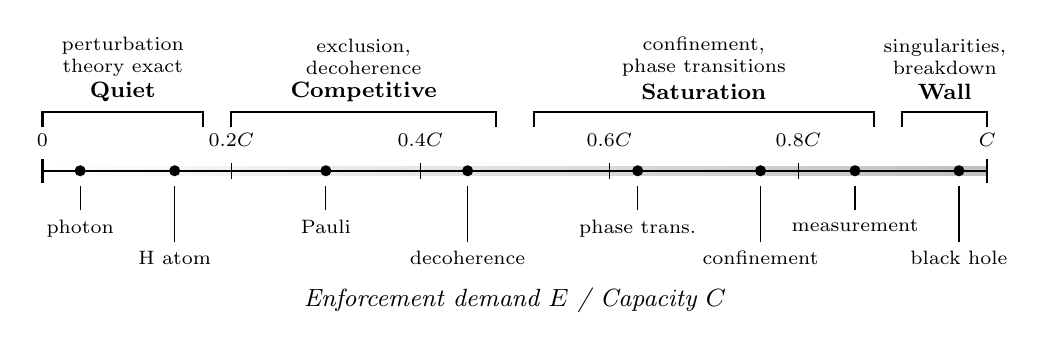
\begin{tikzpicture}[x=12cm, y=1cm]

% --- Gradient shading (behind everything) ---
\shade[left color=white, right color=black!25] (0,-0.06) rectangle (1,0.06);

% --- Main axis ---
\draw[thick] (0,0) -- (1,0);
\draw[thick] (0,-0.15) -- (0,0.15);
\draw[thick] (1,-0.15) -- (1,0.15);

% Tick marks + labels ABOVE axis
\foreach \x/\lab in {0/{0}, 0.2/{0.2$C$}, 0.4/{0.4$C$}, 0.6/{0.6$C$}, 0.8/{0.8$C$}, 1.0/{$C$}} {
  \draw (\x,-0.1) -- (\x,0.1);
  \node[above, font=\scriptsize] at (\x,0.18) {\lab};
}

% --- Regime brackets ---
\draw[thick] (0,0.55) -- (0,0.75) -- (0.17,0.75) -- (0.17,0.55);
\node[font=\footnotesize\bfseries] at (0.085,1.0) {Quiet};
\node[font=\scriptsize, text width=2cm, align=center] at (0.085,1.45) {perturbation\\theory exact};

\draw[thick] (0.20,0.55) -- (0.20,0.75) -- (0.48,0.75) -- (0.48,0.55);
\node[font=\footnotesize\bfseries] at (0.34,1.0) {Competitive};
\node[font=\scriptsize, text width=2.6cm, align=center] at (0.34,1.45) {exclusion,\\decoherence};

\draw[thick] (0.52,0.55) -- (0.52,0.75) -- (0.88,0.75) -- (0.88,0.55);
\node[font=\footnotesize\bfseries] at (0.70,1.0) {Saturation};
\node[font=\scriptsize, text width=2.6cm, align=center] at (0.70,1.45) {confinement,\\phase transitions};

\draw[thick] (0.91,0.55) -- (0.91,0.75) -- (1.0,0.75) -- (1.0,0.55);
\node[font=\footnotesize\bfseries] at (0.955,1.0) {Wall};
\node[font=\scriptsize, text width=1.6cm, align=center] at (0.955,1.45) {singularities,\\breakdown};

% --- System markers: staggered rows ---
\fill (0.04,0) circle (2pt);
\draw (0.04,-0.2) -- (0.04,-0.5);
\node[below, font=\scriptsize, anchor=north] at (0.04,-0.5) {photon};

\fill (0.30,0) circle (2pt);
\draw (0.30,-0.2) -- (0.30,-0.5);
\node[below, font=\scriptsize, anchor=north] at (0.30,-0.5) {Pauli};

\fill (0.63,0) circle (2pt);
\draw (0.63,-0.2) -- (0.63,-0.5);
\node[below, font=\scriptsize, anchor=north] at (0.63,-0.5) {phase trans.};

\fill (0.86,0) circle (2pt);
\draw (0.86,-0.2) -- (0.86,-0.5);
\node[below, font=\scriptsize, anchor=north] at (0.86,-0.5) {measurement};

\fill (0.14,0) circle (2pt);
\draw (0.14,-0.2) -- (0.14,-0.9);
\node[below, font=\scriptsize, anchor=north] at (0.14,-0.9) {H atom};

\fill (0.45,0) circle (2pt);
\draw (0.45,-0.2) -- (0.45,-0.9);
\node[below, font=\scriptsize, anchor=north] at (0.45,-0.9) {decoherence};

\fill (0.76,0) circle (2pt);
\draw (0.76,-0.2) -- (0.76,-0.9);
\node[below, font=\scriptsize, anchor=north] at (0.76,-0.9) {confinement};

\fill (0.97,0) circle (2pt);
\draw (0.97,-0.2) -- (0.97,-0.9);
\node[below, font=\scriptsize, anchor=north] at (0.97,-0.9) {black hole};

% Axis label
\node[font=\small\itshape] at (0.5,-1.65) {Enforcement demand $E$ / Capacity $C$};

% Redraw axis endpoints
\draw[thick] (0,-0.15) -- (0,0.15);
\draw[thick] (1,-0.15) -- (1,0.15);

\end{tikzpicture}

\medskip
\caption{The enforcement spectrum.  Physical systems arranged by the ratio of enforcement demand to capacity ($E/C$).  Standard physics works exactly in the quiet regime ($E/C \ll 1$), requires approximations in the competitive regime ($E/C$ of order unity), and breaks down---singularities, the measurement problem, the information paradox---at the capacity wall ($E/C \to 1$).  The hard problems of physics cluster where $E/C \to 1$.  Regime boundaries are schematic.}
\label{fig:spectrum}
\end{figure}

\medskip\noindent\textbf{The quiet regime ($E/C \ll 1$).}
A single photon maintains two polarization states; a hydrogen atom holds a handful of quantum numbers with well-separated energy levels.  Nothing competes for resources.  Perturbation theory converges, exact solutions exist, and QED predicts the electron's anomalous magnetic moment to 12 decimal places~\cite{Aoyama2020}.  The physics is simple because the local budget is barely taxed.

\medskip\noindent\textbf{The competitive regime ($E/C$ of order unity, below saturation).}
The local budget begins to bind.  Two electrons cannot maintain identical quantum numbers at the same interface because the joint enforcement cost overflows the local budget---the Pauli exclusion principle \emph{is} non-closure ($L_{\mathrm{nc}}$).  Decoherence appears because system--environment correlations commit capacity at both interfaces simultaneously, and the committed capacity is locally unrecoverable~\cite{Zurek2003}.  Perturbation theory still works but requires increasingly sophisticated approximations: the system is managing genuine competition for finite local resources.

\medskip\noindent\textbf{The saturation regime ($E/C$ approaching unity).}
The local budget is nearly exhausted and the physics becomes dramatic.  In QCD, a free quark's unscreened color charge costs more to enforce the further it separates from its partner; when the cost exceeds the local interface capacity, the string snaps and produces color-singlet hadrons---fewer distinctions, lower demand~\cite{Wilson1974}.  At a phase transition, thermal perturbation costs consume the enforcement budget for the ordered state until the interface can no longer afford it and transitions to disorder~\cite{Wilson1983}.  In measurement, cross-system correlations multiply as apparatus and environment entangle, saturating the local budget until only one branch survives~\cite{Zurek1981}.

\medskip\noindent\textbf{The capacity wall ($E/C \to 1$).}
The Bekenstein--Hawking bound $S = A/4\ell_P^2$~\cite{Bekenstein1981} and the APF's $n_{\max} = \lfloor C/\varepsilon^* \rfloor$ are both finite-capacity bounds on the number of independent physical facts a region can support.  The structural parallel is suggestive, but the quantitative mapping---gravitational scaling from enforcement capacity---is the subject of Papers~5--6, not this paper.

\medskip\noindent\textbf{The pattern.}  The standard formalism works beautifully in the quiet regime, requires approximations in the competitive regime, and breaks down---singularities, the measurement problem, the information paradox---at the capacity wall.  These are not separate problems but manifestations of a single structural feature: the standard formalism has no finite local enforcement budget and therefore cannot describe what happens when the budget runs out.  A1 supplies that concept.

\subsection{Context: reconstruction and finite-information programs}
\label{sec:context}

The APF enters a well-established tradition of quantum reconstruction (Hardy~\cite{Hardy2001}; CDP~\cite{CDP2011}; Masanes--M\"uller~\cite{MM2011}; Dakic--Brukner~\cite{DakicBrukner2009}).  These programs derive Hilbert-space formalism from operational axioms within generalized probabilistic theories (GPTs).  The APF begins one step upstream of these programs: \emph{why should physics be a GPT at all?}  A1 derives the convex-probabilistic structure that GPTs assume; the novel chain $L_\Delta \to L_{\mathrm{blk}} \to T_{\mathrm{alg}}$ derives noncommutativity from enforcement costs without assuming algebraic structure.  Two conditions that reconstruction programs take as axioms ($P_{\mathrm{tom}}$, $P_{\mathrm{cls}}$) are here proved as theorems.  A1 is closest in spirit to Bekenstein's entropy bound~\cite{Bekenstein1981}, the holographic principle~\cite{tHooft1993,Susskind1995}, and Jacobson's thermodynamic derivation~\cite{Jacobson1995}.  A detailed GPT cross-reference table is in the Technical Supplement.

Every theorem is implemented as an executable check in the APF codebase (publicly available at \url{https://github.com/Ethan-Brooke}).

\subsection{Road map: from axiom to physics}

\noindent\textit{A narrative walkthrough of the complete argument is given in Section~\ref{sec:argument}.  The table below gives the derivation order; the dependency structure is shown in Figure~\ref{fig:dag}.}

\begin{center}
\captionof{table}{Derivation order of the structural lemmas and bridge theorems.  Rows 7--11 constitute the bridge; the chain's multi-step structure answers the classical-countermodel objection.}
\smallskip
\footnotesize
\setlength{\tabcolsep}{4pt}
\begin{tabular*}{\textwidth}{@{\extracolsep{\fill}}clllll@{}}
\toprule
\textbf{\#} & \textbf{Result} & \textbf{Type} & \textbf{Dependencies} & \textbf{Used by} \\
\midrule
1 & $L_{\mathrm{NZ}}$ (No Zeno) & Lemma & A1 (Aspect~3) & motivation \\
2 & $L_{\varepsilon^*}$ (Min.\ Cost Floor) & Lemma & MD & all below \\
3 & $L_{\mathrm{loc}}$ (Locality) & Lemma & A1, $L_{\varepsilon^*}$, M, $R_{\mathrm{loc}}$ & $L_{\mathrm{irr}}$, Papers 2--7 \\
4 & $L_{\mathrm{nc}}$ (Non-Closure) & Lemma & A1, $L_{\varepsilon^*}$, M & $L_{\mathrm{irr}}$, T1 \\
5 & $L_{\Delta}$ (Competition) & Lemma & A1, SC, CL1--CL3, $T_{\mathrm{sep}}$ & T1, $L_{\mathrm{irr}}$ \\
6 & $L_{\mathrm{irr}}$ (Irreversibility) & Lemma & $L_{\mathrm{nc}}$, $L_\Delta$, $L_{\mathrm{loc}}$ & Papers 3--5 \\
\midrule
\multicolumn{5}{l}{\textit{Bridge: from order-dependence to noncommutative $C^*$-algebra}} \\
\midrule
7 & T1 (Order-Dep.) & Thm & $L_\Delta$, NT, BW & O2 \\
8 & $T_{\mathrm{adj}}$ (Self-Adjoint.) & Thm & $T_{\mathrm{sep}}$, cost additivity & $L_{\mathrm{blk}}$, $L_\Pi$, $T_{\mathrm{alg}}$ \\
8b & $L_{\mathrm{blk}}$ ($\oplus$-Failure) & Thm & $T_{\mathrm{sep}}$, SC, A1, $L_\Delta$ & $T_{\mathrm{alg}}$ (crit.\ path) \\
9 & $L_\Pi$ (Codespace Rot.) & Lemma & $L_\Delta$, OR3, $T_{\mathrm{adj}}$ & FD6 (geom.\ str.) \\
10 & $T_{\mathrm{alg}}$ (Noncomm.) & Thm & $L_{\mathrm{blk}}$, $T_{\mathrm{adj}}$ & T2a \\
11 & $T_{\mathrm{GNS}}$ & Thm & T2a (O3, O4) & T2b, T2c \\
\bottomrule
\end{tabular*}
\label{tab:deriv_order}
\end{center}

These feed into the quantum skeleton: T2a (real $*$-algebra) $\to$ T2b (complexification + Wedderburn--Artin) $\to$ T2c (field selection $\mathbb{C}$).  The bridge rows 7--11 are the multi-step argument that crosses the boundary from operational order-dependence (satisfiable by classical models) to algebraic noncommutativity (not satisfiable by any commutative $*$-algebra).  The classical-countermodel objection is addressed at row~8: $T_{\mathrm{adj}}$ places the enforcement operators \emph{inside} $\mathcal{A}$ as self-adjoint elements; classical models keep their update maps external to the observable algebra, so no self-adjoint enforcement-internal update operator exists (see bridge proofs, Section~\ref{sec:operator_bridge}).

\smallskip\noindent The full assumption inventory --- PLEC's four constitutive features (A1 + MD + A2 + BW) on FD1's enforcement-interface triple, plus the constitutive principles SP and K3 --- is tabulated in Section~\ref{sec:assumption_inventory}.\label{sec:axiom}

\subsubsection*{The three inputs}

The entire framework rests on three stated inputs.  All subsequent structure is derived from these three and nothing else.

\begin{tcolorbox}[apfbox, title={The Principle of Least Enforcement Cost: four structurally necessary components}]

The framework rests on a single variational principle, the \textbf{Principle of Least Enforcement Cost (PLEC)}: \textit{reality is the minimum-cost expression of distinction compatible with finite capacity.}  PLEC is the canonical variational formulation of the enforceability-of-distinction foundation; it does not replace that foundation.  PLEC has four structurally necessary components, each carrying enforceability content independently of PLEC's variational packaging:

\medskip
\textbf{A1} (Finite Enforcement Capacity --- upper bound).  \textit{Every physical fact costs something to maintain, and the total is bounded.}  For any admissible state $\sigma$ on a causally connected region $\Gamma$, the set of physically real distinctions $\mathcal{D}(\sigma,\Gamma) := \{d : \varepsilon(d) > 0\}$ satisfies $|\mathcal{D}| \ge 2$ and $\sum_{d \in \mathcal{D}} \varepsilon(d) \le C(\Gamma) < \infty$.  A1 defines the admissible set.  \coderef{check\_A1}{paper1.py}  A1 is information-theoretic: enforcement cost and capacity $C(\Gamma)$ are counts of maintained distinctions, not energies indexed to an external scale, and every A1-derived quantity in the bank is dimensionless.  Dimensional laboratory predictions inherit their units from APF's Planck-unit convention (see Paper~0 \emph{What Physics Permits} \S``A1 as a statement about information, not energy'' and Paper~13 \emph{The Minimal Admissibility Core} \S``Planck Units as Native Convention'').

\medskip
\textbf{MD} (Enforcement Isotropy --- positive floor).  \textit{The enforcer has no built-in preferred directions.}  There exists $\mu^* > 0$ such that every irreducible distinction costs at least $\mu^*$.  MD is a structural regularity condition analogous to Hardy's continuous reversibility~\cite{Hardy2001}; it is confirmed independently by Paper~6.  \coderef{check\_MD}{paper1.py}

\medskip
\textbf{A2} (Minimum Cost --- argmin).  \textit{Reality sits at the cheapest admissible configuration.}  The physically realized configuration is $G_{\mathrm{realized}}(\rho, \Gamma) = \arg\min_{G \in \mathcal{A}(\rho, \Gamma)} \sum_{d \in G} \varepsilon(d)$.  A2 is the variational-selection component of PLEC.  \coderef{check\_A2}{paper1.py}

\medskip
\textbf{BW} (Budget Window --- non-degeneracy).  \textit{The cost spectrum is rich enough that different enforcement orderings produce distinguishable outcomes.}  There exist three distinctions forming a witnessing triple: $d_3$ is jointly admissible with the cheaper $d_1$ but not with the more expensive $d_2$.  BW is used exactly once (in the proof of T1) and is confirmed by Paper~2's derivation of 61 independent capacity types.  \coderef{check\_BW}{paper1.py}

\medskip
\noindent\textit{Full formal statements, variable definitions, derived consequences, and scope discussions for all four components are in Section~\ref{sec:defs} and the Technical Supplement.}

\end{tcolorbox}

\smallskip\noindent The ``single-principle'' framing is precise: PLEC is a single variational principle whose four components (A1, MD, A2, BW) each carry structurally distinct content---A1 bounds the admissible set from above; MD bounds cost from below; A2 selects the realized configuration by argmin over the admissible set; BW ensures the argmin is non-degenerate.  The definitional layer (FD1--FD6, K1--K4, OR0) and the derived-condition layer (OR1--OR3, SC, $T_{\mathrm{sep}}$, NT, CL1--CL3, P1--P4) are all proved from the components of PLEC plus the definitions.  The detailed defense of this framing, the component essentiality proofs, and the complete label inventory are in the Technical Supplement.

\clearpage
\begin{figure}[p]
\centering
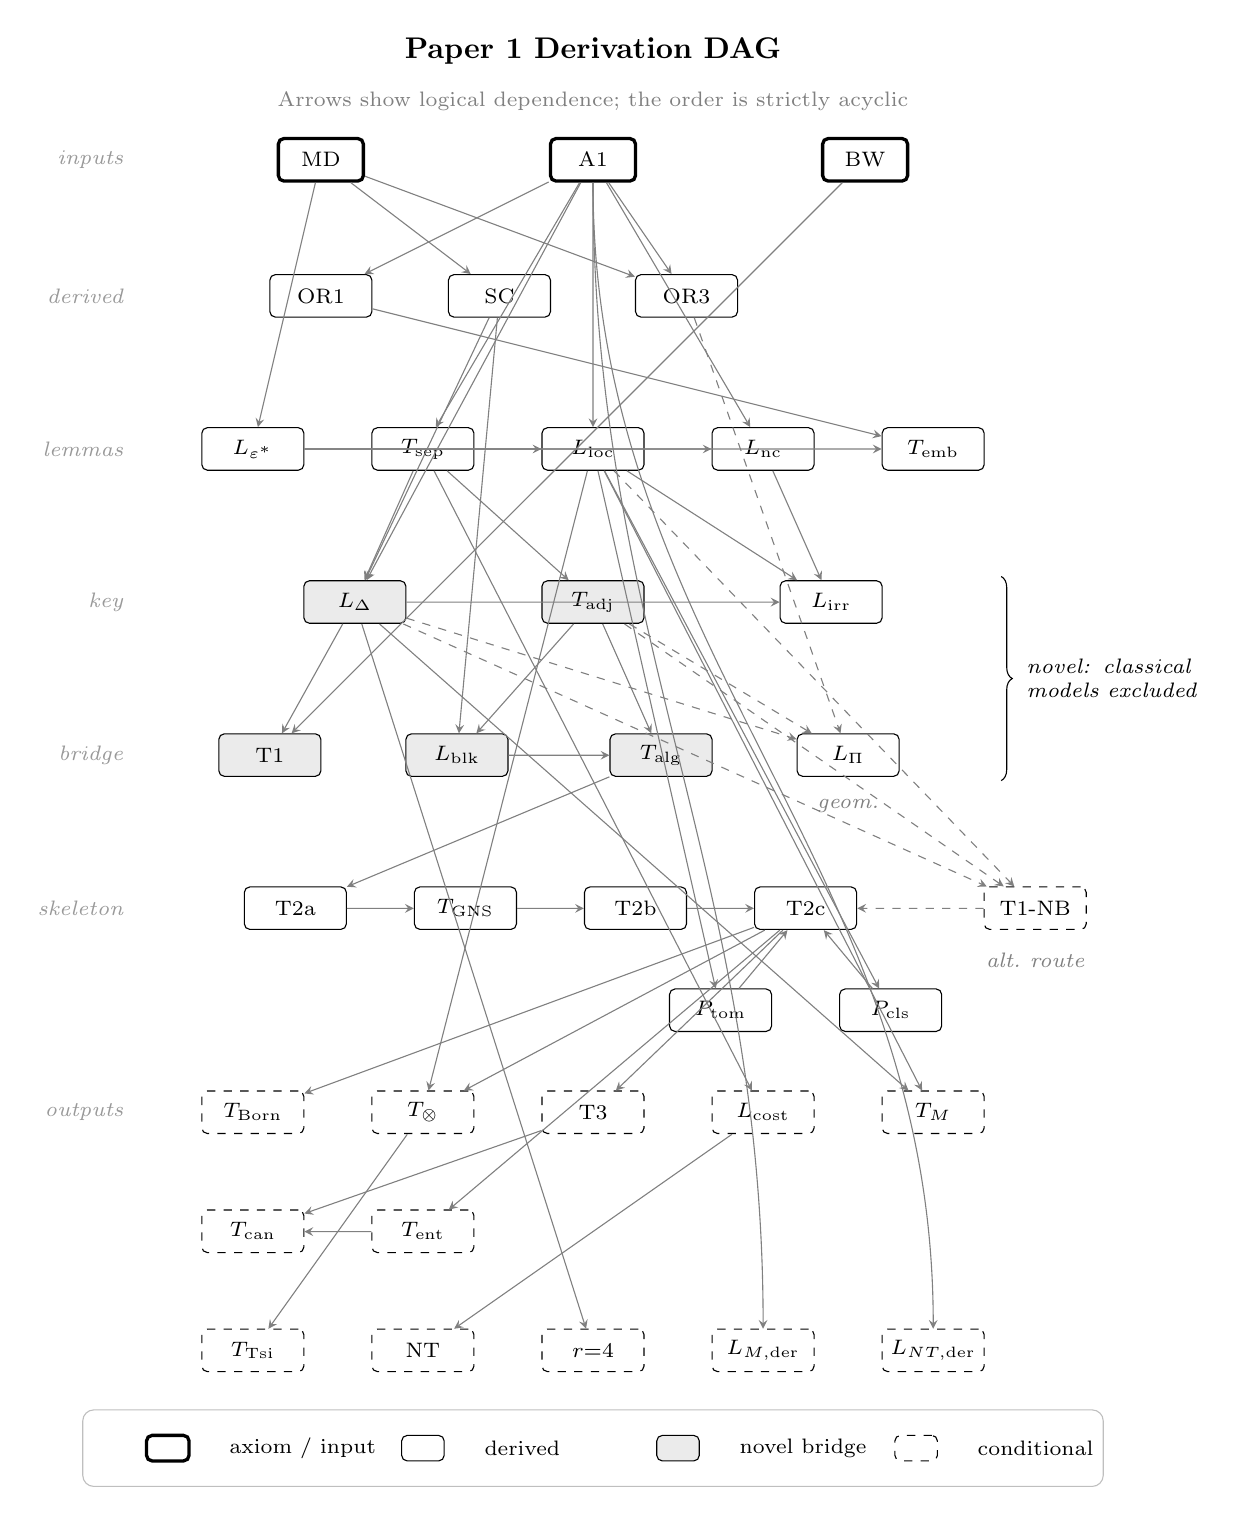
\begin{tikzpicture}[
    scale=1.08, every node/.style={transform shape},
    nd/.style={draw, rounded corners=2pt, minimum height=0.5cm, minimum width=1.2cm, inner sep=2pt, font=\scriptsize},
    input/.style={nd, very thick, minimum width=1.0cm},
    lemma/.style={nd},
    bridge/.style={nd, fill=black!8},
    skel/.style={nd},
    outnode/.style={nd, dashed},
    arr/.style={->, >=stealth, thin, black!50},
    tier/.style={font=\tiny\itshape, anchor=east, text=black!40},
]

% Title
\node[font=\normalsize\bfseries, anchor=south] at (0, 1.0) {Paper 1 Derivation DAG};
\node[font=\scriptsize, anchor=south, text=black!50] at (0, 0.45) {Arrows show logical dependence; the order is strictly acyclic};

% Tier 0: Inputs
\node[tier] at (-5.4, 0) {\scriptsize inputs};
\node[input] (A1) at (0, 0) {A1};
\node[input] (MD) at (-3.2, 0) {MD};
\node[input] (BW) at (3.2, 0) {BW};

% Tier 1: Derived conditions
\node[tier] at (-5.4, -1.6) {\scriptsize derived};
\node[lemma] (OR1) at (-3.2, -1.6) {OR1};
\node[lemma] (SC) at (-1.1, -1.6) {SC};
\node[lemma] (OR3) at (1.1, -1.6) {OR3};

% Tier 2: Structural lemmas
\node[tier] at (-5.4, -3.4) {\scriptsize lemmas};
\node[lemma] (Leps) at (-4.0, -3.4) {$L_{\varepsilon^*}$};
\node[lemma] (Tsep) at (-2.0, -3.4) {$T_{\mathrm{sep}}$};
\node[lemma] (Lloc) at (0.0, -3.4) {$L_{\mathrm{loc}}$};
\node[lemma] (Lnc) at (2.0, -3.4) {$L_{\mathrm{nc}}$};
\node[lemma] (Temb) at (4.0, -3.4) {$T_{\mathrm{emb}}$};

% Tier 2.5: Key lemmas
\node[tier] at (-5.4, -5.2) {\scriptsize key};
\node[bridge] (LDelta) at (-2.8, -5.2) {$L_\Delta$};
\node[bridge] (Tadj) at (0.0, -5.2) {$T_{\mathrm{adj}}$};
\node[lemma] (Lirr) at (2.8, -5.2) {$L_{\mathrm{irr}}$};

% Tier 3: Bridge
\node[tier] at (-5.4, -7.0) {\scriptsize bridge};
\node[bridge] (T1) at (-3.8, -7.0) {T1};
\node[bridge] (Lblk) at (-1.6, -7.0) {$L_{\mathrm{blk}}$};
\node[bridge] (Talg) at (0.8, -7.0) {$T_{\mathrm{alg}}$};
\node[lemma] (LPi) at (3.0, -7.0) {$L_\Pi$};
\node[font=\scriptsize\itshape, gray, anchor=north] at (3.0, -7.4) {geom.};

% Annotation: novel bridge (right side)
\draw[decorate, decoration={brace, amplitude=4pt}]
    (4.8, -4.9) -- (4.8, -7.3)
    node[midway, right=5pt, font=\scriptsize\itshape, text width=2.2cm, align=left] {novel: classical\\models excluded};

% Tier 4: Skeleton
\node[tier] at (-5.4, -8.8) {\scriptsize skeleton};
\node[skel] (T2a) at (-3.5, -8.8) {T2a};
\node[skel] (TGNS) at (-1.5, -8.8) {$T_{\mathrm{GNS}}$};
\node[skel] (T2b) at (0.5, -8.8) {T2b};
\node[skel] (T2c) at (2.5, -8.8) {T2c};
\node[skel, dashed] (T1NB) at (5.2, -8.8) {T1-NB};
\node[font=\scriptsize\itshape, gray, anchor=north] at (5.2, -9.2) {alt.\ route};

% Derived for T2c
\node[lemma] (Ptom) at (1.5, -10.0) {$P_{\mathrm{tom}}$};
\node[lemma] (Pcls) at (3.5, -10.0) {$P_{\mathrm{cls}}$};

% Tier 5: Consequences
\node[tier] at (-5.4, -11.2) {\scriptsize outputs};
\node[outnode] (TBorn) at (-4.0, -11.2) {$T_{\mathrm{Born}}$};
\node[outnode] (Ttens) at (-2.0, -11.2) {$T_{\otimes}$};
\node[outnode] (T3) at (0.0, -11.2) {T3};
\node[outnode] (Lcost) at (2.0, -11.2) {$L_{\mathrm{cost}}$};
\node[outnode] (TM) at (4.0, -11.2) {$T_M$};

% Additional outputs
\node[outnode] (Tcan) at (-4.0, -12.6) {$T_{\mathrm{can}}$};
\node[outnode] (Tentropy) at (-2.0, -12.6) {$T_{\mathrm{ent}}$};

% Terminal
\node[outnode] (Ttsi) at (-4.0, -14.0) {$T_{\mathrm{Tsi}}$};
\node[outnode] (NT) at (-2.0, -14.0) {NT};
\node[outnode] (r4) at (0.0, -14.0) {$r{=}4$};
\node[outnode] (LMder) at (2.0, -14.0) {$L_{M,\mathrm{der}}$};
\node[outnode] (LNTder) at (4.0, -14.0) {$L_{NT,\mathrm{der}}$};

% === ARROWS ===
% Tier 0 → 1
\draw[arr] (A1) -- (OR1);
\draw[arr] (MD) -- (SC);
\draw[arr] (MD) -- (OR3);
\draw[arr] (A1) -- (OR3);

% Tier 0/1 → 2
\draw[arr] (MD) -- (Leps);
\draw[arr] (A1) -- (Tsep);
\draw[arr] (A1) -- (Lloc);
\draw[arr] (Leps) -- (Lloc);
\draw[arr] (A1) -- (Lnc);
\draw[arr] (Leps) -- (Lnc);
\draw[arr] (OR1) -- (Temb);
\draw[arr] (Leps) -- (Temb);

% → key lemmas
\draw[arr] (SC) -- (LDelta);
\draw[arr] (Tsep) -- (LDelta);
\draw[arr] (A1) -- (LDelta);
\draw[arr] (Tsep) -- (Tadj);
\draw[arr] (LDelta) -- (Lirr);
\draw[arr] (Lnc) -- (Lirr);
\draw[arr] (Lloc) -- (Lirr);

% → bridge
\draw[arr] (LDelta) -- (T1);
\draw[arr] (BW) -- (T1);
\draw[arr] (Tadj) -- (Lblk);
\draw[arr] (SC) -- (Lblk);
\draw[arr] (Lblk) -- (Talg);
\draw[arr] (Tadj) -- (Talg);
\draw[arr, gray, dashed] (LDelta) -- (LPi);
\draw[arr, gray, dashed] (Tadj) -- (LPi);
\draw[arr, gray, dashed] (OR3) -- (LPi);

% bridge → skeleton
\draw[arr] (Talg) -- (T2a);
\draw[arr] (T2a) -- (TGNS);
\draw[arr] (TGNS) -- (T2b);
\draw[arr] (T2b) -- (T2c);
\draw[arr] (Ptom) -- (T2c);
\draw[arr] (Pcls) -- (T2c);
\draw[arr] (Lloc) -- (Ptom);
\draw[arr] (Lloc) -- (Pcls);

% skeleton → outputs
\draw[arr] (T2c) -- (TBorn);
\draw[arr] (T2c) -- (Ttens);
\draw[arr] (Lloc) -- (Ttens);
\draw[arr] (T2c) -- (T3);
\draw[arr] (Tsep) -- (Lcost);
\draw[arr] (Lloc) -- (TM);
\draw[arr] (LDelta) -- (TM);

% → T1-NB (alternative route)
\draw[arr, dashed] (LDelta) -- (T1NB);
\draw[arr, dashed] (Lloc) -- (T1NB);
\draw[arr, dashed] (Tadj) -- (T1NB);
\draw[arr, dashed] (T1NB) -- (T2c);

% → additional outputs
\draw[arr] (T2c) -- (Tentropy);
\draw[arr] (T3) -- (Tcan);
\draw[arr] (Tentropy) -- (Tcan);

% → terminal
\draw[arr] (Ttens) -- (Ttsi);
\draw[arr] (Lcost) -- (NT);
\draw[arr] (LDelta) -- (r4);
\draw[arr] (A1) to[out=-90, in=90] (LMder);
\draw[arr] (A1) to[out=-90, in=90] (LNTder);

% === LEGEND ===
\draw[black!25, rounded corners=4pt] (-6.0, -15.6) rectangle (6.0, -14.7);
\node[input, minimum width=0.5cm, minimum height=0.3cm] at (-5.0, -15.15) {};
\node[font=\scriptsize, anchor=west] at (-4.4, -15.15) {axiom / input};
\node[lemma, minimum width=0.5cm, minimum height=0.3cm] at (-2.0, -15.15) {};
\node[font=\scriptsize, anchor=west] at (-1.4, -15.15) {derived};
\node[bridge, minimum width=0.5cm, minimum height=0.3cm] at (1.0, -15.15) {};
\node[font=\scriptsize, anchor=west] at (1.6, -15.15) {novel bridge};
\node[outnode, minimum width=0.5cm, minimum height=0.3cm] at (3.8, -15.15) {};
\node[font=\scriptsize, anchor=west] at (4.4, -15.15) {conditional};

\end{tikzpicture}
\caption[Paper~1 Derivation DAG]{%
\textbf{Paper~1 Derivation DAG.}
Every arrow is a logical dependency; the graph is strictly acyclic.
The three inputs (thick border) are
\textbf{A1}~(Finite Enforcement Capacity),
\textbf{MD}~(Enforcement Isotropy),
and \textbf{BW}~(Budget Window); all other nodes are derived.
The shaded bridge chain ($L_\Delta \to T_{\mathrm{adj}} \to L_{\mathrm{blk}} \to T_{\mathrm{alg}}$) is the novel core of the paper: this is where faithful commuting-extension defenders for the tested interface are excluded.  ($L_\Pi$ provides geometric strengthening but is not on the critical path.)
Two independent branches --- quantum structure (left, via~$L_\Delta$) and locality/gauge (right, via~$L_{\mathrm{loc}}$) --- converge at T2c.
T1-NB (dashed) is the independent Non-Boolean route to the algebra (Choquet $\to$ Vinberg $\to$ Albert).
$T_{\mathrm{can}}$, $T_{\mathrm{ent}}$ (entropy), $L_{M,\mathrm{der}}$, and $L_{NT,\mathrm{der}}$ are consequence-level results.
Dashed output nodes are conditional on the identifications of \S\ref{sec:identifications}.
}
\label{fig:dag}
\end{figure}
\clearpage

% ======================================================================

\begin{tcolorbox}[apfbox, title={Descriptive-framing convention (read once, applies throughout)}]
In the derivation chapters that follow, the verbs ``forces,'' ``selects,'' ``rejects,'' and ``enforces'' are used as shorthand for uniqueness and $\arg\min$ results over the space of A1-admissible configurations.  ``A1 forces $X$'' means: $X$ is the unique admissible value given A1, and any alternative is inadmissible by the stated definitions.  No process of enforcement is being described.  ``Enforcement'' names the cost structure $\varepsilon(d)$; it does not denote an agent or a mechanism.  The shorthand is retained because replacing it sentence by sentence would obscure the proof structure; the reader should interpret every ``forces'' below as an $\arg\min$ or uniqueness claim.  The ontology reading is: what exists is the minimum-cost configuration consistent with the capacity bound, in the same descriptive sense that a classical trajectory is the path of stationary action.
\end{tcolorbox}

% ======================================================================
\section{Definitions and structural lemmas}
\label{sec:defs}
% ======================================================================

\begin{tcolorbox}[apfbox, title={Operational primitives: where each term is defined and formalized}]
This paper builds on three operational primitives.  Each is motivated in
\S 1, formalized below in \S 2, and exploited in the bridge of \S 3.
The box is a wayfinder, not new content; every claim points to where in
the paper the term is defined or formalized.

\begin{description}[topsep=2pt,itemsep=2pt]
  \item[Distinction.]  A binary partition of admissible configurations at
    an interface --- ``this'' versus ``not this'' in the sense of
    Spencer-Brown.  \emph{Motivated:} \S 1.1 ``The finite universe''
    (Zeeman-protected spin, ionization-protected atom, mass-protected
    nucleon, barrier-protected localization).  \emph{Formalized:} FD2
    (binary-predicate structure, \S\ref{sec:defs}); the structural-lemma
    family $T_{\mathrm{sep}}$, $L_{\mathrm{loc}}$, NT, and
    $L_{\mathrm{nc}}$.

  \item[Maintained.]  Held against perturbation by ongoing commitment of
    enforcement cost.  Maintenance is not a one-time setup; the cost is
    paid moment-to-moment.  \emph{Motivated:} \S 1.1 (``actively
    maintained --- kept true, moment to moment, against everything that
    would blur it out'').  \emph{Formalized:} $L_{\varepsilon^*}$
    minimum-cost floor (\S\ref{sec:eps_star}); $L_{\mathrm{cost}}$
    cost-functional uniqueness (\S\ref{sec:L_cost}).

  \item[Enforcement cost $\varepsilon(d)$.]  The minimum capacity required
    to maintain the distinction $d$.  Resource-agnostic at the framework
    level: in laboratory instances $\varepsilon$ appears as energy
    (Zeeman gap), binding energy (ionization), mass difference (nucleon),
    or potential height (localization), but the framework specifies
    $\varepsilon$ as a real-valued functional, not a particular SI quantity.
    \emph{Axiomatized:} A1 with capacity bound $C(\Gamma) < \infty$
    (\S 1.1; formal box \S\ref{sec:defs}).  \emph{Functional form derived:}
    $L_{\mathrm{cost}}$ (\S\ref{sec:L_cost}) ---
    $\varepsilon(d) = n(d)\cdot\varepsilon^*$ with no free parameter.
    \emph{Measurement protocol:} Technical Supplement.
\end{description}
\end{tcolorbox}

\subsection{Enforceability and its variational expression}
\label{sec:input_grounding}

\smallskip\noindent\textbf{\S2.0\quad The admissibility structure as the arena of PLEC.}  A1, MD, A2, BW, and FD1--FD6 together characterize the \emph{admissibility structure} at each interface: A1 and MD define the admissible set from above and below (enforceability side); A2 selects the argmin within it, and BW guarantees that argmin is non-degenerate (variational side).  The unified content of these four components is the \textbf{Principle of Least Enforcement Cost} --- \textit{realization $=$ argmin over admissible configurations, where admissibility is set by finite enforcement capacity and a positive cost floor.}  $L_{\mathrm{loc}}$ stitches per-interface admissibility structures into a global one; physical reality is its realized element.  The remainder of \S2 develops these components in order---inputs first (\S2.1), derived vocabulary second (FD1--FD6 summary), structural lemmas third.

\medskip\noindent The derivation rests on the \textbf{Principle of Least Enforcement Cost (PLEC)}, decomposed into four structurally necessary components---A1 (upper bound on admissibility), MD (positive cost floor), A2 (argmin selection), BW (non-degeneracy)---together with six foundational definitions (FD1--FD6).  Each component is stated here with its core physical content.  PLEC is the variational formulation of the enforceability-of-distinction foundation; its four components are separately sufficient for distinct structural roles and together produce the admissibility argmin.  Detailed physical grounding (A1's two internal regimes, $\varepsilon(d) > 0$ at $T = 0$, Zeno considerations, four independent corroborations of the $\mathcal{D}$-quotient, worked examples of perturbation classes, the extended MD discussion, countermodel analysis, and A2's descriptive-vs-selective status) is in the Technical Supplement.\label{assumption:MD}%
\label{cor:disjoint_mech}

Enforceability of Distinction (with its finite-capacity and positive-floor features, A1 and MD) is the ontological foundation; PLEC is its variational formulation, expressed through the argmin (A2) over an admissible set made non-degenerate by BW.  Both the ontological foundation and its variational formulation are load-bearing: every result in this paper traces back to one or more of PLEC's four components.  A1, MD, A2, BW are each structurally necessary---none is derivable from the others (see Technical Supplement essentiality proofs, and Paper~0's \emph{PLEC component decomposition} table, which compresses ``what each component adds and what removing it breaks'' into one lookup and is the intended rebuttal of the ``APF derives everything from A1 alone'' misreading).

\begin{tcolorbox}[defbox, title={Axiom A1 (Finite Enforcement Capacity)}]
The total enforcement cost of all simultaneously maintained distinctions at any interface $\Gamma$ is bounded:
\[
\sum_{d \in \mathcal{D}(\sigma,\Gamma)} \varepsilon(d) \;\le\; C(\Gamma), \qquad 0 < C(\Gamma) < \infty, \qquad |\mathcal{D}| \ge 2.
\]
A distinction $d$ is \emph{physically real} iff $\varepsilon(d) > 0$.  The state space $\Omega$ is the $\mathcal{D}$-quotient: two configurations agreeing on all $d \in \mathcal{D}$ are the same physical state (Proposition~\ref{prop:D_quotient_forced}, proved in the Technical Supplement from the standard GPT quotienting procedure with $\mathcal{D}$ as effect set).  A1 does not specify whether the universe is classical or quantum, continuous or discrete, four-dimensional or otherwise---all such properties are derived in Sections~\ref{sec:defs}--\ref{sec:skeleton}.
\end{tcolorbox}

\smallskip\noindent A1 bounds the admissible configurations from above but does not say which admissible configuration is realized.  Two configurations at different total costs both satisfy A1.  The step from \emph{admissible} to \emph{realized}---the step every ``A1 forces $X$'' argument had left implicit---is named explicitly by A2.

\begin{tcolorbox}[defbox, title={Axiom A2 (Minimum Cost)}]
Let $\mathcal{A}(\rho, \Gamma)$ denote the admissible set at interface $\Gamma$ in state $\rho$---the set of configurations satisfying A1.  The physically realized configuration is
\[
G_{\mathrm{realized}}(\rho, \Gamma) \;=\; \operatorname*{arg\,min}_{G \in \mathcal{A}(\rho, \Gamma)} \sum_{d \in G} \varepsilon(d).
\]

\smallskip\noindent\textit{What A2 says.}  A descriptive predicate naming the location of physical reality within the admissible set: reality sits at the argmin, not at some other admissible point.  A2 is parametric in $(\rho, \Gamma)$---one statement per interface.  Globality is obtained by gluing per-interface admissibility structures via $L_{\mathrm{loc}}$, not by a separate global claim.

\smallskip\noindent\textit{What A2 does not say.}  A2 does not describe a selection mechanism.  No agent ranges over candidates; no dynamical search is performed.  The verification procedure (enumerate, exhibit the argmin) is an artifact of proof, not a physical process---parallel to how the principle of stationary action is descriptive of the classical trajectory rather than prescriptive of how it was computed.

\smallskip\noindent\textit{Tie-breaking.}  When the argmin is not a singleton, A2 alone is silent; downstream uniqueness theorems (anomaly cancellation, Witten parity, $T_{\mathrm{gauge}}$, $T_{\mathrm{field}}$) establish uniqueness structurally.

\smallskip\noindent\textit{Why A2 is not derived from A1 or MD.}  A1 bounds from above but does not discriminate among admissible configurations with different total costs.  MD imposes a positive cost floor but does not assert that total cost is minimized.  Neither alone, nor both together, imply A2.  The ``realized $=$ argmin'' claim is new information; hence A2 must be stated.
\end{tcolorbox}

\smallskip\noindent A1 and A2 fix the shape of the framework: what is admissible (A1) and what is realized (A2).  What remains is the cost structure itself.  A1 tells us the budget is finite but says nothing about how cost distributes across directions.  Without a second condition, a single direction could consume arbitrarily little cost while others bear the full weight.  MD closes this gap.

\begin{tcolorbox}[defbox, title={Structural Assumption MD (Enforcement Isotropy)}]
There exists $\mu^* > 0$ such that for every $d \in \mathcal{D}$:
\[
\varepsilon(d) \;\geq\; \mu^* \cdot n(d),
\]
where $n(d) \ge 1$ is the \emph{enforcement complexity} (minimum independent binary tests to specify $d$'s status).  After the vector space is constructed (OR3), $n(d) = \dim(M_d)$.  MD is the single structural assumption beyond A1 in this paper.  Its pre-geometric form uses only the operational quantity $n(d)$, not the linear-algebraic $\dim(M_d)$; the identification is confirmed downstream, not presupposed (non-circularity argument in the Technical Supplement).

\smallskip\noindent\textit{What MD says.}  Every unit of enforcement complexity costs at least $\mu^*$ to maintain, uniformly across all distinctions.  \textit{What MD rules out.}  The countermodel $\varepsilon(d_n) = 1/2^n$ with $n(d_n) = 1$: every cost is positive but $\varepsilon^* = 0$, permitting infinitely many independent distinctions.  MD excludes this by requiring a complexity-independent cost floor.  Full discussion in Section~\ref{sec:MD_detail}.
\end{tcolorbox}

\smallskip\noindent MD converts the abstract finiteness of A1 into a uniform floor: every direction pays at least its fair share.  This is the condition that will produce the minimum cost $L_{\varepsilon^*}$ and, ultimately, discrete structure.

\smallskip\noindent A1 and MD together produce a finite, isotropic cost spectrum.  BW asks only that this spectrum is not degenerate---that at least three distinct cost values exist, providing a budget window between them.

\begin{tcolorbox}[defbox, title={Richness Premise BW (Budget Window)}]
The cost spectrum $\{\varepsilon(d) : d \in \mathcal{D}\}$ contains at least one witnessing triple $(d_1, d_2, d_3)$ with $\varepsilon(d_1) < \varepsilon(d_2)$ such that $d_3$ is jointly admissible with $d_1$ but not with $d_2$: the distinction $d_3$ lives in the \emph{budget window} between the two residual budgets.  BW converts abstract algebraic noncommutativity into physically observable order-dependence.  Used exactly once: in the proof of T1 (Section~\ref{sec:L_Delta}).  BW fails only for degenerate cost spectra (measure-zero condition) and is confirmed by Paper~2's 61 independent capacity types.
\end{tcolorbox}

\smallskip\noindent The three inputs define the rules of the game.  What follows is the vocabulary---five formal primitives that name the objects the framework talks about.  These are not additional assumptions; each is either a direct naming of something A1 already implies (FD1--FD4) or a constitutive construction from the definitions (FD5).  With the vocabulary in place, the first structural result---the separation biconditional---establishes the geometric meaning of independence.

\medskip\noindent\textbf{Definitional layer: five primitives (FD1--FD5).}
The framework's vocabulary consists of five definitions whose detailed formal specifications, type signatures, and constitutive derivations are in the Technical Supplement.  The summary:

\smallskip
\begin{tabular*}{\textwidth}{@{\extracolsep{\fill}}lll@{}}
\textbf{Prim.} & \textbf{Name} & \textbf{Content} \\[2pt]
\hline\noalign{\smallskip}
FD1 & Interface $\Gamma$ & $(S_\Gamma, C(\Gamma))$: substrate + budget; FD1a (set), FD1b (vec.\ space) \\[3pt]
FD2 & Distinction $d$ & $d: S_\Gamma \to \{0,1\}$; real iff $\varepsilon(d) > 0$ \\[3pt]
FD3 & Anchor set $M_d$ & Min.\ subspace $M_d \subseteq S_\Gamma$; all perturbation supports for $d$ \\[3pt]
FD4 & Enf.\ cost & $\varepsilon(d) := \inf\{\kappa(p)\}$; $\kappa$ satisfies K1--K4 (derived) \\[3pt]
FD5 & Enf.\ op.\ $E_d$ & FD5a: idempotent, $\mathrm{im}(E_d)\!=\!M_d$; FD5b: proj.\ $\pi_{M_d}$ \\
\end{tabular*}

\label{box:formal_spec}%
\label{prop:D_quotient_forced}%
\label{prop:FD1_derived}%
\label{prop:FD4_constitutive}%
\label{defn:Dsigma}%
\label{prop:meas}

\smallskip\noindent An \emph{admissible state} $\sigma = (S_\sigma, \delta_\sigma) \in \Omega(\Gamma)$ has independently enforceable active set $S_\sigma \in \mathcal{D}_{\mathrm{ind}}$ and residual budget $\delta_\sigma = C(\Gamma) - \sum_{d \in S_\sigma} \varepsilon(d) \ge 0$.  The active distinction set $\mathcal{D}(\sigma,\Gamma) := S_\sigma$ is well-defined, independent, and finite: $|\mathcal{D}(\sigma,\Gamma)| \le \lfloor C/\varepsilon^* \rfloor < \infty$ (Theorem D-fin).  Full formal specifications, the $\mathcal{D}$-quotient proposition, constitutive derivations, and perturbation lemmas P1--P4 are in the Technical Supplement.

\begin{tcolorbox}[apfbox, title={Theorem $T_{\mathrm{sep}}$ (Separation Biconditional)}]
\textit{Two distinctions have additive enforcement costs iff their mechanisms occupy disjoint substrate regions.}

\smallskip\noindent\textbf{Statement.}  $\mathcal{P}(d) \cap \mathcal{P}_\Gamma = \emptyset$ for all $d$ $\;\Longleftrightarrow\;$ $M_d \cap M_{d'} = \{0\}$ for all $d \ne d'$.
\begin{equation}
M_d \cap M_{d'} = \{0\} \qquad \forall\; d \neq d' \in \mathcal{D}(\Gamma).
\label{eq:disjoint_support}
\end{equation}

\smallskip\noindent\textbf{Depends on.}  FD3, FD4.  \textbf{Status.}  \textbf{[Proved]} from A1 + definitions (both directions; see Technical Supplement).

\smallskip\noindent\textbf{Corollary.}  $L_\Delta$ and T1 hold exactly in the disjoint-mechanism regime ($\mathcal{D}_{\mathrm{ind}}$).  In the overlapping regime ($M_d \cap M_{d'} \ne \{0\}$), the budget sum overcounts, $\Delta \le 0$ is possible, and the algebra is commutative (worked example in Section~\ref{sec:overlap_detail}).
\end{tcolorbox}

\smallskip\noindent $T_{\mathrm{sep}}$ translates the accounting concept of additive cost into a geometric concept: disjoint mechanism support.  Every result in the cost-lemma chain that follows---$L_{\varepsilon^*}$, $L_{\mathrm{cost}}$, $L_{\mathrm{loc}}$, NT---rests on this biconditional.  And when we reach $L_\Delta$, it is exactly the failure of $T_{\mathrm{sep}}$'s disjoint condition that creates the interference that forces quantum structure.

\begin{figure}[ht]
\centering
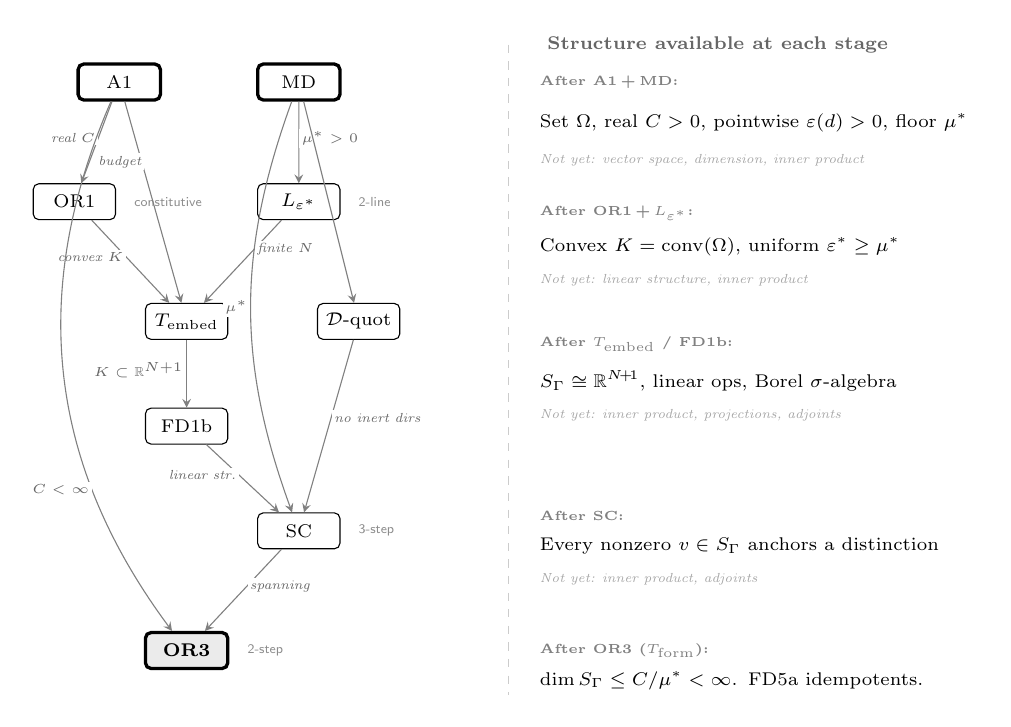
\begin{tikzpicture}[
    scale=0.95, every node/.style={transform shape},
    nd/.style={draw, rounded corners=2pt, minimum height=0.48cm, minimum width=1.1cm, inner sep=2pt, font=\scriptsize},
    input/.style={nd, very thick},
    derived/.style={nd},
    target/.style={nd, fill=black!8, very thick},
    arr/.style={->, >=stealth, thin, black!50},
    elabel/.style={font=\tiny\itshape, text=black!60, fill=white, inner sep=1pt},
    badge/.style={font=\tiny, text=black!45, anchor=west},
    inventory/.style={font=\scriptsize, anchor=west, text width=5.8cm, align=left},
    invlabel/.style={font=\tiny\bfseries, anchor=west, text=black!50},
    noyet/.style={font=\tiny\itshape, text=black!35, anchor=west},
]

% ── Nodes (left half) ──
\node[input] (A1) at (0, 0) {A1};
\node[input] (MD) at (2.4, 0) {MD};

\node[derived] (OR1) at (-0.6, -1.6) {OR1};
\node[derived] (Leps) at (2.4, -1.6) {$L_{\varepsilon^*}$};

\node[derived] (Temb) at (0.9, -3.2) {$T_{\mathrm{embed}}$};
\node[derived] (FD1b) at (0.9, -4.6) {FD1b};

\node[derived] (Dquot) at (3.2, -3.2) {$\mathcal{D}$-quot};
\node[derived] (SC) at (2.4, -6.0) {SC};

\node[target] (OR3) at (0.9, -7.6) {\textbf{OR3}};

% ── Proof-type badges ──
\node[badge] at ($(OR1.east)+(0.12,0)$) {\textsf{constitutive}};
\node[badge] at ($(Leps.east)+(0.12,0)$) {\textsf{2-line}};
\node[badge] at ($(SC.east)+(0.12,0)$) {\textsf{3-step}};
\node[badge] at ($(OR3.east)+(0.12,0)$) {\textsf{2-step}};

% ── Arrows with edge labels ──
\draw[arr] (A1) -- node[elabel, left, pos=0.45] {real $C$} (OR1);
\draw[arr] (MD) -- node[elabel, right, pos=0.45] {$\mu^* > 0$} (Leps);
\draw[arr] (OR1) -- node[elabel, left, pos=0.45] {convex $K$} (Temb);
\draw[arr] (Leps) -- node[elabel, right, pos=0.35] {finite $N$} (Temb);
\draw[arr] (A1) -- node[elabel, left=-1pt, pos=0.3] {budget} (Temb);
\draw[arr] (Temb) -- node[elabel, left, pos=0.45] {$K \subset \mathbb{R}^{N+1}$} (FD1b);
\draw[arr] (MD) -- (Dquot);
\draw[arr] (FD1b) -- node[elabel, left, pos=0.45] {linear str.} (SC);
\draw[arr] (Dquot) -- node[elabel, right, pos=0.45] {no inert dirs} (SC);
\draw[arr] (MD) to[bend right=20] node[elabel, left, pos=0.5] {$\mu^*$} (SC);
\draw[arr] (A1) to[bend right=30] node[elabel, left, pos=0.72] {$C < \infty$} (OR3);
\draw[arr] (SC) -- node[elabel, right, pos=0.45] {spanning} (OR3);

% ── Structure inventory (right panel) ──
\draw[black!20, dashed] (5.2, 0.5) -- (5.2, -8.2);
\node[font=\scriptsize\bfseries, text=black!60] at (8.0, 0.5) {Structure available at each stage};

\node[invlabel] at (5.5, -0.0) {After A1\,+\,MD:};
\node[inventory] at (5.5, -0.55) {Set $\Omega$, real $C > 0$, pointwise $\varepsilon(d) > 0$, floor $\mu^*$};
\node[noyet] at (5.5, -1.05) {Not yet: vector space, dimension, inner product};

\node[invlabel] at (5.5, -1.75) {After OR1\,+\,$L_{\varepsilon^*}$:};
\node[inventory] at (5.5, -2.2) {Convex $K = \mathrm{conv}(\Omega)$, uniform $\varepsilon^* \ge \mu^*$};
\node[noyet] at (5.5, -2.65) {Not yet: linear structure, inner product};

\node[invlabel] at (5.5, -3.5) {After $T_{\mathrm{embed}}$ / FD1b:};
\node[inventory] at (5.5, -4.0) {$S_\Gamma \cong \mathbb{R}^{N\!+\!1}$, linear ops, Borel $\sigma$-algebra};
\node[noyet] at (5.5, -4.45) {Not yet: inner product, projections, adjoints};

\node[invlabel] at (5.5, -5.8) {After SC:};
\node[inventory] at (5.5, -6.2) {Every nonzero $v \in S_\Gamma$ anchors a distinction};
\node[noyet] at (5.5, -6.65) {Not yet: inner product, adjoints};

\node[invlabel] at (5.5, -7.6) {After OR3 ($T_{\mathrm{form}}$):};
\node[inventory] at (5.5, -8.0) {$\dim S_\Gamma \le C/\mu^* < \infty$.  FD5a idempotents.};

\end{tikzpicture}
\caption[Arena chain]{%
\textbf{Arena chain: from finite budget to finite-dimensional substrate.}
Each arrow is labelled with the structure it provides.
Right panel: the running inventory of available mathematical structure at each stage.
Inner products, orthogonal projections, and adjoints appear \emph{nowhere} in this chain;
they enter only at $T_{\mathrm{adj}}$ (Figure~\ref{fig:bridge_dag}).
}
\label{fig:arena_dag}
\end{figure}

\smallskip\noindent\textbf{Proposition SC} (Substrate Completeness)\textbf{.}  Every nonzero $v \in S_\Gamma$ anchors a distinction with $\varepsilon(d_v) > 0$.  Proved from MD + $\mathcal{D}$-quotient + FD1b in three steps (Technical Supplement).  Essential downstream: feeds into $T_{\mathrm{form}}$ and $L_\Delta$.
\label{prop:SC}

\smallskip\noindent\textbf{Theorem $T_{\mathrm{embed}}$} (Canonical Embedding)\textbf{.}  The abstract state set $\Omega$ embeds injectively into $\mathbb{R}^{N+1}$ with $N \le \lfloor C/\varepsilon^*\rfloor$, preserving cost data and yielding a compact convex state space.  Proof: constructive (Technical Supplement).
\label{thm:T_embed}

This finite-dimensional structure has a direct engineering consequence for superconducting quantum circuits.  A transmon qubit with anharmonicity $\alpha$ and transition frequency $\omega_{01}$ operated at temperature $T$ has $n_{\mathrm{max}} = \lfloor C(\Gamma)/\varepsilon^* \rfloor$ physically enforceable energy levels, where $C(\Gamma)$ is set by the total electromagnetic energy budget of the interface and $\varepsilon^*$ by the minimum energy gap resolvable against thermal noise.  The standard practice of truncating transmon simulations to 3--5 levels reflects this physical $n_{\mathrm{max}}$, not a numerical convenience: levels above $n_{\mathrm{max}}$ cannot be independently maintained against perturbation at finite capacity, and adding them to a simulation does not add physical content.

\smallskip\noindent\textbf{Theorem OR3} ($T_{\mathrm{form}}$: Finite Substrate)\textbf{.}  $\dim(S_\Gamma) \le C(\Gamma)/\mu^* < \infty$.

\smallskip\noindent\textit{Proof sketch.}  Let $\{v_1, \ldots, v_k\}$ be any linearly independent set in $S_\Gamma$.  By SC, each $v_i$ anchors an irreducible distinction $d_{v_i}$ with $M_{d_{v_i}} = \mathrm{span}\{v_i\}$.  Linear independence gives $M_{d_{v_i}} \cap M_{d_{v_j}} = \{0\}$, so $\{d_{v_1}, \ldots, d_{v_k}\}$ is independently enforceable.  By MD: $\sum_i \varepsilon(d_{v_i}) \ge k\mu^*$.  By A1: $k\mu^* \le C(\Gamma)$.  Hence $k \le C/\mu^*$ for every linearly independent set, giving $\dim(S_\Gamma) \le C/\mu^* < \infty$.  \hfill$\square$

\smallskip\noindent\textbf{Proposition} (Disjoint Partition)\textbf{.}\label{prop:disjoint_partition}  Distinct interfaces have disjoint substrates: $S_{\Gamma_1} \cap S_{\Gamma_2} = \emptyset$.  Proved from A1 + $L_{\mathrm{cost}}$'s integrality: the minimum cost quantum $\varepsilon^*$ is indivisible across interfaces.  See Technical Supplement.

\smallskip\noindent\textbf{Independence}\label{def:independence} operates at two levels: \emph{within-interface} ($d_1 \perp d_2 \Leftrightarrow M_{d_1} \cap M_{d_2} = \{0\}$, characterized by $T_{\mathrm{sep}}$) and \emph{between-interface} ($S_{\Gamma_1} \cap S_{\Gamma_2} = \emptyset$, from the Disjoint Partition).  The richness premise $R_{\mathrm{loc}}$ ($N_{\mathrm{phys}} > \lfloor C_{\max}/\varepsilon^* \rfloor$) forces distribution across multiple interfaces; it is confirmed by Paper~2's 61 capacity types.


\subsection{Structural lemmas of the arena}
\label{sec:lemmas}

The five structural lemmas derive from A1 and MD alone; no companion-paper result is required.  The three-layer architecture (Layer~1: A1 + MD; Layer~2: definitions FD1--FD5; Layer~3: derived structure) ensures clean separation between physical axiom, definitional semantics, and mathematical consequences.

\subsection{\texorpdfstring{$L_{\varepsilon^*}$}{L epsilon*} (Minimum Cost Floor): no infinitesimal distinctions}
\label{sec:eps_star}

\noindent $T_{\mathrm{sep}}$ gives us geometric independence; the next step is to show that this independence imposes a minimum price.  Without a floor on enforcement cost, an adversary could maintain infinitely many distinctions at negligible cost each, and the finiteness of A1 would have no structural bite.

\begin{tcolorbox}[apfbox, title={$L_{\varepsilon^*}$ (Minimum Cost Floor) --- Theorem}]
\label{sec:logical_status_eps_star}
\textit{No distinction can be maintained for free: there is a uniform positive floor on all enforcement costs.}

\smallskip\noindent\textbf{Statement.}  There exists $\varepsilon^* > 0$ such that $\varepsilon(d) \ge \varepsilon^* > 0$ for all $d \in \mathcal{D}$.

\smallskip\noindent\textbf{Depends on.}  MD only.  \textbf{Status.}  \textbf{[Proved]} --- two lines.

\smallskip\noindent\textbf{Proof.}  By MD: $\varepsilon(d) \ge \mu^* \cdot n(d) \ge \mu^* \cdot 1 = \mu^*$ for every $d \in \mathcal{D}$ (since $n(d) \ge 1$).  Therefore $\varepsilon^* := \inf_d \varepsilon(d) \ge \mu^* > 0$.  No finiteness of $\mathcal{D}$ is invoked.  \hfill$\square$

\smallskip\noindent\textbf{Consequence.}  $|S_\sigma| \le \lfloor C(\Gamma)/\varepsilon^* \rfloor < \infty$ for every admissible state.

\smallskip\noindent\textbf{Downstream.}  $T_{\mathrm{embed}}$ (finite $N$), $T_{\mathrm{form}}$/OR3 ($\dim S_\Gamma < \infty$), $L_{\mathrm{cost}}$, $L_{\mathrm{loc}}$.

\smallskip\noindent\textit{Why A1 alone does not suffice}: pointwise $\varepsilon(d) > 0$ on an infinite index set does not imply a uniform floor ($\varepsilon(d_n) = 1/n$ is a counterexample).  MD closes the gap.  The no-Zeno lemma $L_{\mathrm{NZ}}$ (enforcement histories terminate) is proved from A1's operational content but does not establish $\varepsilon^* > 0$; see Technical Supplement.  By $L_{\mathrm{cost}}$ (below), $\varepsilon^*$ cancels from all dimensionless predictions.

\coderef{check\_L\_epsilon\_star}{paper1.py}
\end{tcolorbox}

\smallskip\noindent This is the first structural consequence of A1: a discrete cost spectrum that eventually produces quantum granularity.  But discreteness alone is not enough---we need to know that the cost function itself is unique.

\begin{tcolorbox}[apfbox, title={From a floor to a ladder: why $L_{\varepsilon^*}$ needs $L_{\mathrm{cost}}$}]
$L_{\varepsilon^*}$ delivers a positive floor $\mu^* > 0$: no admissible distinction costs less than the minimum quantum.  This is necessary but not sufficient for predictive content.  A floor alone permits costs of $\mu^*$, $2.73\,\mu^*$, $\pi\,\mu^*$, $17\,\mu^*$ --- any positive real above the floor.  Cost assignments would remain a free parameter, undoing the variational compactness PLEC's four constitutive features supply (A1 bound + MD floor + A2 argmin + BW non-degeneracy on FD1's enforcement-interface structure).

\smallskip\noindent $L_{\mathrm{cost}}$ closes the gap.  From additivity ($T_{\mathrm{sep}}$) and the binary-predicate structure (FD2), the Cauchy functional equation on $\mathbb{N}$ fixes the cost functional: every admissible cost is an integer multiple of $\mu^*$.  The free parameters collapse to a single scale.

\smallskip\noindent\textbf{Physical anchor: Planck's step.}\quad In 1900, Planck showed that blackbody radiation required energies bounded below by a minimum $h\nu$ --- the floor.  But what his formula actually fits is the stronger statement $E = n h\nu$, energies in integer multiples.  The step from ``minimum energy exists'' to ``energies are integer-indexed'' is not a technical refinement; it is the arrival of quantization itself.  The atomic Rydberg series ($E_n = -13.6\,\mathrm{eV}/n^2$) and the phonon spectrum in solids carry the same structure: a single quantum plus integer multiplicity, with no free parameter between them.

\smallskip\noindent $L_{\mathrm{cost}}$ is the framework's analogue of Planck's step.  Cost space is a ladder, not a floor.
\end{tcolorbox}

\subsection{\texorpdfstring{$L_{\mathrm{cost}}$}{L cost}: cost functional uniqueness}
\label{sec:L_cost}\label{sec:L_map}

\noindent A minimum cost quantum exists ($L_{\varepsilon^*}$); $T_{\mathrm{sep}}$ makes costs additive over disjoint supports.  The next result shows that these two facts leave no freedom: the cost of any structure is an integer multiple of the minimum, with no adjustable parameters.

\begin{tcolorbox}[apfbox, title={$L_{\mathrm{cost}}$: Cost Functional Form Uniqueness}]
\textit{The enforcement cost of any structure is an integer multiple of the minimum cost quantum --- forced by the Cauchy functional equation on $\mathbb{N}$.}

\smallskip\noindent\textbf{Statement.}  The cost functional has the unique form $C(E) = n(E) \cdot \varepsilon^*$, where $n(E) \in \mathbb{N}$ is the number of independent enforcement channels and $\varepsilon^* := f(1) > 0$.

\smallskip\noindent\textbf{Depends on.}  A1, MD ($\Rightarrow$ C1: ledger completeness), binary-predicate structure ($\Rightarrow$ C1b: integrality), $T_{\mathrm{sep}}$ ($\Rightarrow$ C2: additive independence).

\smallskip\noindent\textbf{Status.}  \textbf{[Proved]}.  The Cauchy equation $f(n_1 + n_2) = f(n_1) + f(n_2)$ on $\mathbb{N}$ has unique solution $f(n) = nf(1)$ by induction; no regularity condition is needed (the domain is $\mathbb{N}$, not $\mathbb{R}$).

\smallskip\noindent\textbf{Proof sketch.}  Sub-lemma~C1 (from A1 + MD): $C(E) = f(n(E))$ depends only on channel count.  Sub-lemma~C1b (from FD2): $n(E) \in \mathbb{N}$ since each distinction is a binary predicate contributing 0 or 1 channels.  Sub-lemma~C2 (from $T_{\mathrm{sep}}$): $f(n_1 + n_2) = f(n_1) + f(n_2)$ for independent structures.  On $\mathbb{N}$, the single generator $1$ gives $f(n) = nf(1) = n\varepsilon^*$ by induction.  \hfill$\square$

\smallskip\noindent\textbf{Downstream.}  Disjoint Partition (substrate exclusivity), $L_{\mathrm{loc}}$, NT, Cost Discreteness.  Full sub-lemma proofs, scope delimitation (V1--V3 criteria), and physical-domain verifications are in the Technical Supplement.

\coderef{check\_L\_cost}{paper1.py}\,%
\hspace{1em}\textit{(also verified in \texttt{supplement.py})}
\end{tcolorbox}

\smallskip\noindent Cost uniqueness means the framework has no free parameters at this level---every physical proxy for enforcement cost is proportional to the same integer channel count.  The next step is to show that this cost distributes locally.

\subsection{\texorpdfstring{$L_{\mathrm{loc}}$}{L loc} (Locality): enforcement must distribute}
\label{sec:L_loc}

\noindent Cost is quantised ($L_{\varepsilon^*}$) and unique ($L_{\mathrm{cost}}$).  The next lemma shows it is also local: each interface manages its own budget, with no capacity transfer between disjoint substrates.

\begin{tcolorbox}[apfbox, title={Lemma $L_{\mathrm{loc}}$ (Locality)}]
\textit{Independent interfaces have independent budgets: no enforcement act at one interface can affect another.}

\smallskip\noindent\textbf{Statement.}  For any two interfaces $\Gamma_1, \Gamma_2$ with disjoint enforcement substrates ($S_{\Gamma_1} \cap S_{\Gamma_2} = \emptyset$), the enforcement budgets are independent: $C(\Gamma_1 \cup \Gamma_2) = C(\Gamma_1) + C(\Gamma_2)$.  Consequently, the state space factorizes: $\Omega(\Gamma_1 \cup \Gamma_2) \cong \Omega(\Gamma_1) \times \Omega(\Gamma_2)$.

\smallskip\noindent\textbf{Depends on.}  $T_{\mathrm{sep}}$ (disjoint anchor sets), $L_{\mathrm{cost}}$ (cost functional uniqueness), $\mathcal{D}$-quotient definition of $\Omega$.  Disjoint substrates are themselves derived from A1 + $L_{\mathrm{cost}}$ (Proposition~\ref{prop:disjoint_partition}).

\smallskip\noindent\textbf{Status.}  \textbf{[Proved]} --- full proof in Technical Supplement, Theorem~$L_{\mathrm{loc}}$.

\smallskip\noindent\textbf{Proof sketch} (three steps).

\textit{Step 1 (Budget additivity).}  Disjoint substrates + $T_{\mathrm{sep}}$ give disjoint anchor sets across interfaces.  By $L_{\mathrm{cost}}$, capacity counts channels: $C(E) = n(E)\varepsilon^*$.  Channel counts add over disjoint supports, so $C(\Gamma_1 \cup \Gamma_2) = C(\Gamma_1) + C(\Gamma_2)$.

\textit{Step 2 (No inter-interface capacity transfer).}  Perturbations at $\Gamma_1$ act only on $S_{\Gamma_1}$; by disjointness they leave $S_{\Gamma_2}$ unchanged.  Budget consumed at one interface cannot substitute for budget at another.

\textit{Step 3 (State-space factorization).}  An explicit bijection $\Omega(\Gamma_1 \cup \Gamma_2) \cong \Omega(\Gamma_1) \times \Omega(\Gamma_2)$ is constructed from the $\mathcal{D}$-quotient: restrict the active set and residual budget to each interface.  Well-definedness, injectivity, and surjectivity follow from Steps~1--2.  \hfill$\square$

\coderef{check\_L\_loc}{paper1.py}\,%
\hspace{1em}\textit{(also verified in \texttt{supplement.py})}
\end{tcolorbox}

\smallskip\noindent Locality converts the global constraint of A1 into a local one: each interface manages its own budget.  With cost unique and local, we can now prove that the cost spectrum is genuinely non-degenerate.

% ======================================================================
% NT: moved here from the skeleton section. NT depends on L_cost + SC + A1,
% all available above. T1 (in the bridge) needs NT.
% ======================================================================

\subsection{Theorem NT (Non-Degeneracy): proof from $L_{\mathrm{cost}}$}
\label{sec:NT_proof}

With $L_{\mathrm{cost}}$ established, the non-degeneracy theorem NT can now be proved.  If every distinction had the same cost, the budget window of BW would collapse and order-dependence could not arise.  NT closes this gap: compound distinctions exist with higher dimension and therefore higher cost.

\begin{tcolorbox}[apfbox, title={Theorem NT (Non-Degeneracy) --- Proof}]
\textit{The enforcement cost spectrum is not constant: there exist distinctions with different costs.}

\smallskip\noindent\textbf{Statement.}  There exist distinctions $d_i, d_j \in \mathcal{D}$ with $\varepsilon(d_i) \ne \varepsilon(d_j)$.

\smallskip\noindent\textbf{Depends on.}  A1 ($|\mathcal{D}| \ge 2$), $T_{\mathrm{sep}}$ (disjoint anchors for independent distinctions), SC (every nonzero direction anchors a distinction), $L_{\mathrm{cost}}$ ($\varepsilon(d) = \dim(M_d) \cdot \varepsilon^*$).

\smallskip\noindent\textbf{Status.}  \textbf{[Proved]} from A1 + $L_{\mathrm{cost}}$ + SC.  Previously listed as a sub-clause of A1; now derived.

\smallskip\noindent\textbf{Downstream.}  Used in: T1 (order-dependence requires non-degenerate cost spectrum to produce a budget-window witness).

\smallskip\noindent\textbf{Proof.}  By A1, $|\mathcal{D}| \ge 2$: there exist at least two irreducible distinctions $d_1, d_2 \in \mathcal{D}$ with $\dim(M_{d_1}) = \dim(M_{d_2}) = 1$.  By $T_{\mathrm{sep}}$, their anchor sets are disjoint: $M_{d_1} \cap M_{d_2} = \{0\}$.

Consider the compound predicate $d_{12}: S_\Gamma \to \{0,1\}$ defined by $d_{12}(\sigma) = 1$ iff $d_1(\sigma) = 1$ or $d_2(\sigma) = 1$.  Its anchor set is $M_{d_{12}} = M_{d_1} \oplus M_{d_2}$, which has $\dim(M_{d_{12}}) = 2$.  By SC, $\varepsilon(d_{12}) > 0$, so $d_{12} \in \mathcal{D}$.

By $L_{\mathrm{cost}}$: $\varepsilon(d_{12}) = \dim(M_{d_{12}}) \cdot \varepsilon^* = 2\varepsilon^*$ and $\varepsilon(d_1) = \dim(M_{d_1}) \cdot \varepsilon^* = \varepsilon^*$.  Therefore $\varepsilon(d_{12}) = 2\varepsilon^* \ne \varepsilon^* = \varepsilon(d_1)$.  \hfill$\square$

\coderef{check\_NT}{paper1.py}
\end{tcolorbox}

\smallskip\noindent Non-degeneracy is the last piece of the classical infrastructure.  Everything up to this point---minimum cost, cost uniqueness, locality, non-degeneracy---could in principle hold in a classical world.  The next result is where that possibility begins to close.

\subsection{\texorpdfstring{$L_{\mathrm{nc}}$}{L nc} (Non-Closure): composition overflows capacity}
\label{sec:L_nc}

\noindent The five lemmas above build the arena: finite, discrete, unique, local, non-degenerate.  $L_{\mathrm{nc}}$ draws the first consequence that will matter for the bridge: finite budgets can overflow.

\begin{tcolorbox}[apfbox, title={Lemma $L_{\mathrm{nc}}$ (Non-Closure)}]
\textit{Two individually affordable distinctions can be jointly unaffordable --- the state space is not closed under arbitrary combination.}

\smallskip\noindent\textbf{Statement.}  Let $\Gamma$ be an interface with $|\mathcal{D}(\Gamma)| \ge 2$ and two distinctions $d_1, d_2 \in \mathcal{D}(\Gamma)$ satisfying $\varepsilon(d_1) + \varepsilon(d_2) > C(\Gamma)$.  Then $\Omega_{\mathrm{adm}}$ is not closed under convex combinations of states involving $d_1$ and $d_2$.

\smallskip\noindent\textbf{Depends on.}  A1 (finite budget), FD4 (positive enforcement costs).  No other results required --- this is the simplest consequence of finite capacity.

\smallskip\noindent\textbf{Status.}  \textbf{[Proved]} --- direct budget-overflow argument.  Classical; no quantum structure involved.

\smallskip\noindent\textit{Proof.}  Let $d_1, d_2 \in \mathcal{D}(\Gamma)$ be co-located distinctions with individual costs $\varepsilon(d_1), \varepsilon(d_2) > 0$ satisfying $\varepsilon(d_1) + \varepsilon(d_2) > C(\Gamma)$.  (Such a pair exists whenever $|\mathcal{D}(\Gamma)| \ge 2$ and the total individual cost exceeds the budget; A1 makes $C(\Gamma)$ finite while the individual costs are positive by FD4.)  Then both $\sigma_1 = (\{d_1\}, C(\Gamma) - \varepsilon(d_1)) \in \Omega_{\mathrm{adm}}$ and $\sigma_2 = (\{d_2\}, C(\Gamma) - \varepsilon(d_2)) \in \Omega_{\mathrm{adm}}$ are individually admissible.  The midpoint $\tfrac{1}{2}\sigma_1 + \tfrac{1}{2}\sigma_2$ would correspond to simultaneously enforcing both $d_1$ and $d_2$ at equal weight, requiring total cost at least $\varepsilon(d_1) + \varepsilon(d_2) > C(\Gamma)$: inadmissible.  Therefore $\Omega_{\mathrm{adm}}$ is not convex.

\smallskip\noindent\textit{Note.}  This proof uses only A1 (finite budget) and FD4 (positive enforcement costs); it invokes neither the perturbation structure of Lemmas~P1--P4 nor the strict superadditivity of $L_\Delta$.  Non-closure is therefore a purely classical consequence of finite budgets, present in any knapsack-type resource model.  In convex resource cone terms: the admissible state set $\Omega_{\mathrm{adm}}$ is \emph{not} a convex cone---the midpoint of two extreme rays lies outside $\Omega_{\mathrm{adm}}$ whenever the combined cost exceeds $C(\Gamma)$.  $L_\Delta$ (proved in the next section) establishes the strictly stronger quantum regime: \emph{strict} superadditivity, which requires the additional structure of co-located disjoint mechanisms.  \hfill$\square$

\coderef{check\_L\_nc}{paper1.py}
\end{tcolorbox}

\noindent\textit{What $L_{\mathrm{nc}}$ establishes and what it leaves open.}  Non-closure is the weakest structural consequence of A1: some combinations of individually admissible states are collectively inadmissible.  This is the classical knapsack regime --- overflow without interference, without superadditivity, without any structure that distinguishes quantum from classical.

\medskip

\begin{tcolorbox}[apfbox, title={The gap between $L_{\mathrm{nc}}$ and $L_\Delta$: where classical models end}]
$L_{\mathrm{nc}}$ established that finite budgets can overflow --- that some combinations of individually admissible distinctions cost more than the capacity allows.  This is a purely classical resource phenomenon: any knapsack model produces the same overflow, and no quantum structure is implicated.

\smallskip\noindent The strictly stronger result --- that co-located distinctions incur a superadditive cost premium $\Delta > 0$ \emph{even when their individual enforcement mechanisms are disjoint} --- is the content of $L_\Delta$, proved in the next section.  The gap between $L_{\mathrm{nc}}$ (overflow) and $L_\Delta$ (superadditivity) is exactly where classical models end and quantum structure begins.

\smallskip\noindent The distinction is ontological, not technical.  Classical resource models treat co-located distinctions as independent bookkeeping entries: the cost of maintaining both is the sum of maintaining each.  $L_\Delta$ commits the framework to something stronger --- that co-location at a shared interface creates a cost beyond the sum, produced by the integrity requirement on the shared substrate itself.  Two physical examples anchor the claim.

\smallskip\noindent\textbf{Example 1: Pauli exclusion as superadditive cost.}\quad Two electrons confined to a single atomic orbital are enforced by disjoint mechanisms: each electron's presence is a distinct labelled distinction, with its own cost of localization against escape.  Classically, the combined cost would be twice the single-electron cost --- each electron separately maintained at its site.  In reality, the antisymmetrization requirement on the joint wavefunction introduces an \emph{exchange energy}: a cost not present in either single-electron case and not predicted by any additive bookkeeping.  This is a superadditive premium $\Delta > 0$: co-enforcing two presence-distinctions at the same spatial interface costs more than the sum of the individual presence-costs, even though the individual mechanisms --- one electron versus the other --- are themselves disjoint.  The shared orbital is what carries the premium; without commitment to it as a single substrate, the exchange term has no structural home.

\smallskip\noindent\textbf{Example 2: The uncertainty relation as superadditive cost.}\quad Position and momentum of a single particle are enforced by disjoint mechanisms: rulers versus recoils, distinct operators acting on distinct aspects of the state.  Classically, the cost of a sharp position distinction and the cost of a sharp momentum distinction would be independent, and co-enforcing both at the same particle would cost no more than the sum.  Quantum mechanics instead imposes the uncertainty relation $\Delta x \, \Delta p \ge \hbar/2$, a floor on the combined uncertainty-product that no amount of technical refinement escapes.  This is not a measurement limitation imposed from outside the framework --- it is $L_\Delta$ at the finest possible resolution: the surplus cost of co-enforcing two disjoint-mechanism distinctions at the same particle-interface.  The single-particle state is the shared substrate, and $\hbar/2$ is the minimum premium its integrity requires.

\smallskip\noindent In each case, disjoint mechanisms are not enough to purchase independence.  Co-location at a shared interface forces the mechanisms to share the interface's integrity budget, and the integrity budget cannot serve both without premium.  $L_\Delta$ names this structural fact; the remainder of this paper traces its consequences.
\end{tcolorbox}
% LP proof demoted to constructive verification.
% Replaces lines ~1296–1595 of Paper_1_core_v15_3__3_.tex
% ======================================================================

% ======================================================================

\medskip\noindent\textit{End of the definitional layer.}  The formal bridge
(Section~\ref{sec:formal_bridge}) uses only the structures defined above:
A1, MD, BW, the definitions FD1--FD5 and FD4b, the structural lemmas
$T_{\mathrm{sep}}$, SC, $T_{\mathrm{embed}}$, $T_{\mathrm{form}}$/OR3,
$L_{\varepsilon^*}$, $L_{\mathrm{cost}}$, NT, $L_{\mathrm{loc}}$, and
$L_{\mathrm{nc}}$.  No perturbation model (K1--K4, P1--P4), no LP
decomposition, no toy model, and no companion-paper result is required.
FD6 (joint enforcement operation) is derived within the bridge from
$L_\Pi$ and does not appear here.


% ======================================================================
\section{The formal bridge: from finite capacity to noncommutative continuation structure}
\label{sec:formal_bridge}\label{sec:bridge}
% ======================================================================

\noindent The definitional layer is now in place.  This section uses it to derive the noncommutative continuation structure of finite tested (IJC) interfaces: five structural lemmas, and the three-step bridge from order-dependence to noncommutativity ($T_{\mathrm{adj}} \to L_{\mathrm{blk}} \to T_{\mathrm{alg}}$).  The only inputs are A1, MD, BW, and the definitions and lemmas of Section~\ref{sec:defs}.  Full proofs are in the Technical Supplement; proof sketches ($\le 20$ lines each) are given here.  The standard representation-theoretic ascent from the resulting noncommutative continuation algebra to a complex Hilbert representation, the Born rule, and Tsirelson-type bounds is previewed in the subsections that follow Theorem $T_{\mathrm{alg}}$; full formal development of those preview steps is deferred to the quantum-structure paper.  The dependency structure is shown in Figure~\ref{fig:formal_bridge_dag}.

% Bridge DAG (main figure)
\begin{figure}[ht]
\centering
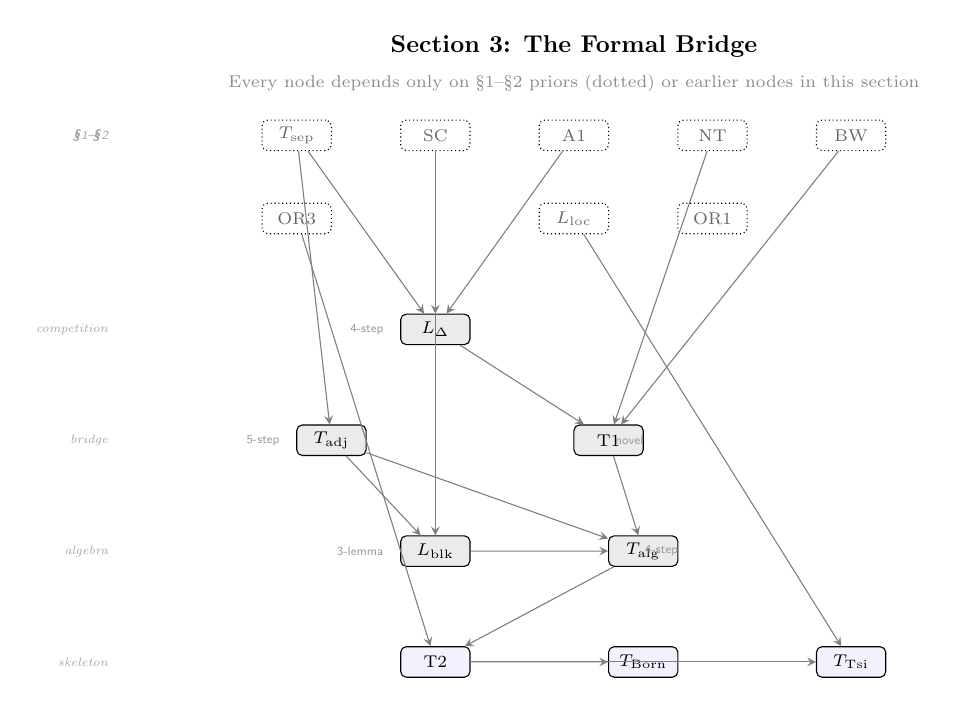
\begin{tikzpicture}[
    scale=0.88, every node/.style={transform shape},
    nd/.style={draw, rounded corners=2pt, minimum height=0.44cm, minimum width=1.0cm, inner sep=2pt, font=\scriptsize},
    prior/.style={nd, densely dotted, text=black!60},
    bridge/.style={nd, fill=black!8},
    skel/.style={nd, fill=blue!5},
    outnode/.style={nd, fill=green!5},
    arr/.style={->, >=stealth, thin, black!50},
    elabel/.style={font=\tiny\itshape, text=black!55, fill=white, inner sep=1pt},
    badge/.style={font=\tiny, text=black!40, anchor=east},
    tier/.style={font=\tiny\itshape, anchor=east, text=black!35},
]

\node[font=\normalsize\bfseries, anchor=south] at (1.0, 1.0)
    {Section 3: The Formal Bridge};
\node[font=\scriptsize, anchor=south, text=black!45] at (1.0, 0.5)
    {Every node depends only on \S1--\S2 priors (dotted) or earlier nodes in this section};

% TIER 0: Prior results from §1 and §2 (dotted)
\node[tier] at (-5.6, 0) {{\fontsize{5}{6}\selectfont\textsf{\S1--\S2}}};
\node[prior] (Tsep) at (-3.0, 0) {$T_{\mathrm{sep}}$};
\node[prior] (SC) at (-1.0, 0) {SC};
\node[prior] (A1) at (1.0, 0) {A1};
\node[prior] (NT) at (3.0, 0) {NT};
\node[prior] (BW) at (5.0, 0) {BW};
\node[prior] (OR3) at (-3.0, -1.2) {OR3};
\node[prior] (Lloc) at (1.0, -1.2) {$L_{\mathrm{loc}}$};
\node[prior] (OR1) at (3.0, -1.2) {OR1};

% TIER 1: Superadditivity
\node[tier] at (-5.6, -2.8) {{\fontsize{5}{6}\selectfont competition}};
\node[bridge] (LDelta) at (-1.0, -2.8) {$L_\Delta$};
\node[badge] at ($(LDelta.west)+(-0.12,0)$) {\textsf{4-step}};

% TIER 2: Order-dependence + self-adjointness
\node[tier] at (-5.6, -4.4) {{\fontsize{5}{6}\selectfont bridge}};
\node[bridge] (T1) at (1.5, -4.4) {T1};
\node[bridge] (Tadj) at (-2.5, -4.4) {$T_{\mathrm{adj}}$};
\node[badge] at ($(T1.east)+(0.12,0)$) {\textsf{novel}};
\node[badge] at ($(Tadj.west)+(-0.12,0)$) {\textsf{5-step}};

% TIER 3: Noncommutativity proof
\node[tier] at (-5.6, -6.0) {{\fontsize{5}{6}\selectfont algebra}};
\node[bridge] (Lblk) at (-1.0, -6.0) {$L_{\mathrm{blk}}$};
\node[bridge] (Talg) at (2.0, -6.0) {$T_{\mathrm{alg}}$};
\node[badge] at ($(Lblk.west)+(-0.12,0)$) {\textsf{3-lemma}};
\node[badge] at ($(Talg.east)+(0.12,0)$) {\textsf{4-step}};

% TIER 4: Representation
\node[tier] at (-5.6, -7.6) {{\fontsize{5}{6}\selectfont skeleton}};
\node[skel] (T2) at (-1.0, -7.6) {T2};
\node[skel] (TBorn) at (2.0, -7.6) {$T_{\mathrm{Born}}$};
\node[skel] (TTsi) at (5.0, -7.6) {$T_{\mathrm{Tsi}}$};

% Arrows
\draw[arr] (Tsep) -- (LDelta);
\draw[arr] (SC) -- (LDelta);
\draw[arr] (A1) -- (LDelta);
\draw[arr] (LDelta) -- (T1);
\draw[arr] (NT) -- (T1);
\draw[arr] (BW) -- (T1);
\draw[arr] (Tsep) -- (Tadj);
\draw[arr] (Tadj) -- (Lblk);
\draw[arr] (SC) -- (Lblk);
\draw[arr] (Lblk) -- (Talg);
\draw[arr] (Tadj) -- (Talg);
\draw[arr] (T1) -- (Talg);
\draw[arr] (Talg) -- (T2);
\draw[arr] (OR3) -- (T2);
\draw[arr] (T2) -- (TBorn);
\draw[arr] (T2) -- (TTsi);
\draw[arr] (Lloc) -- (TTsi);

\end{tikzpicture}
\caption[Formal bridge]{%
\textbf{The formal bridge: from finite budget to quantum mechanics.}
Dotted nodes are §1--§2 priors; shaded nodes are the novel bridge steps.
The chain is: $L_\Delta$ (superadditivity) $\to$ T1 (order-dependence) + $T_{\mathrm{adj}}$ (self-adjointness) $\to$ $L_{\mathrm{blk}} + T_{\mathrm{alg}}$ (noncommutativity) $\to$ T2 (Hilbert space) $\to$ $T_{\mathrm{Born}}$ + $T_{\mathrm{Tsirelson}}$.
}
\label{fig:formal_bridge_dag}
\end{figure}


% ======================================================================
\subsection{\texorpdfstring{$L_{\Delta}$}{L Delta} (Competition): superadditivity from substrate integrity}
\label{thm:ldelta}\label{sec:L_Delta}

Everything derived so far is consistent with a classical world---a world where enforcement costs simply add and distinctions never interfere.  The next result ends that possibility.  When two distinctions share a substrate, maintaining both costs more than maintaining each separately.  The surplus arises not from any interaction Hamiltonian or coupling constant, but from the geometry of defence: protecting the shared substrate against perturbation requires coordinated action that no independent strategy can replicate.  This superadditivity is the seed of quantum mechanics.

\begin{tcolorbox}[apfbox, title={$L_{\Delta}$ (Competition): Superadditivity from Substrate Integrity}]
\textit{Co-located distinctions with disjoint mechanisms cost strictly more together than apart.}

\smallskip\noindent\textbf{Definition (Co-location).}  Distinctions $d_1, d_2$ are \emph{co-located at $\Gamma$} if: (CL1) $M_{d_1}, M_{d_2} \subseteq S_\Gamma$; (CL2) $M_{d_1} \cap M_{d_2} = \{0\}$ ($T_{\mathrm{sep}}$); (CL3) $\Pi := S_\Gamma \setminus (M_{d_1} \oplus M_{d_2}) \ne \emptyset$ (residual substrate exists; guaranteed when $n_{\max} \ge 3$, Lemma~\ref{prop:generic_coloc}).\label{prop:generic_coloc}

\smallskip\noindent\textbf{Statement.}  For co-located $d_1, d_2$:
\begin{equation}\label{eq:Ldelta}
\varepsilon(\{d_1, d_2\}) = \varepsilon(d_1) + \varepsilon(d_2) + \Delta(d_1,d_2), \qquad \Delta = \varepsilon(d_\Gamma) > 0,
\end{equation}
where $d_\Gamma$ is the substrate-integrity distinction on $\Pi$.

\smallskip\noindent\textbf{Depends on.}  A1, $T_{\mathrm{sep}}$, SC.  \textbf{Status.}  \textbf{[Proved]} --- four steps.

\smallskip\noindent\textbf{Proof sketch.}  \textit{Step 1}: CL3 gives a pool $\Pi \ne \{0\}$ beyond $M_{d_1} \oplus M_{d_2}$. \textit{Step 2}: by SC, $\Pi$ anchors a distinction $d_\Gamma$ with $\varepsilon(d_\Gamma) > 0$.  \textit{Step 3}: defending both $d_1$ and $d_2$ requires also defending pool integrity $d_\Gamma$ (a perturbation acting on $\Pi$ can corrupt both mechanisms via the shared substrate).  \textit{Step 4}: by $T_{\mathrm{sep}}$, costs over disjoint anchors add, giving $\varepsilon(\{d_1,d_2\}) \ge \varepsilon(d_1) + \varepsilon(d_2) + \varepsilon(d_\Gamma) > \varepsilon(d_1) + \varepsilon(d_2)$.  \hfill$\square$

\smallskip\noindent Full proof with LP verification in Technical Supplement.  Constructive verifications (toric code, qubit, two-register harmonic oscillator) in Section~\ref{sec:Ldelta_verifications}.

\coderef{check\_L\_Delta}{paper1.py}
\end{tcolorbox}

\begin{tcolorbox}[apfbox, title={Physical anchor: coupled superconducting resonators as an $L_\Delta$ instance}]
Mead's analysis of two coupled superconducting resonators (\cite{Mead2000}, \S\S 4.5--4.8) instantiates the $L_\Delta$ pattern in a system where the shared substrate is explicit and the coupling is quantitatively derivable from first principles.

\smallskip\noindent Each resonator is an $LC$ circuit with flux $\Phi_i$ satisfying (\cite{Mead2000} Eq.~4.18)
\[
LC\,\ddot{\Phi}_i + \Phi_i = \phi_i,
\]
where $\phi_i$ is the four-potential contribution from the other resonator via the retarded/advanced Green's function (Eq.~4.20).  Substituting gives the coupled equations (Eq.~4.22)
\[
\tau^2 \ddot{\Phi}_1 + \Phi_1 = \delta\tau^4\,\partial_t^4 \Phi_2, \qquad \tau^2 \ddot{\Phi}_2 + \Phi_2 = \delta\tau^4\,\partial_t^4 \Phi_1,
\]
with $\tau^2 = LC$ and coupling constant $\delta = \mu_0 l^4/(8\pi r c^2 L^2 C)$.  The normal modes are $\omega_{1,2}^2 \approx \omega_0^2(1 \mp \delta)$ (Eq.~4.27), and the slow-amplitude dynamics (Eq.~4.31) are $\partial_t a_1 = -\delta\omega_0 a_2$, $\partial_t a_2 = +\delta\omega_0 a_1$.

\smallskip\noindent\textbf{Structural mapping to $L_\Delta$.}\quad The two distinctions are ``resonator~1 oscillates with amplitude $a_1$'' and ``resonator~2 oscillates with amplitude $a_2$.''  Their disjoint mechanisms are the two self-flux terms $LI_i$ in Mead's decomposition $\Phi_i = LI_i + \phi_i$ (Eq.~4.17): each resonator's self-inductance contribution is localized to that resonator.  The shared substrate --- the pool $\Pi$ --- is the four-potential $\phi$ through which the two currents influence each other, visible in Eq.~4.20 as the Green's-function coupling.  The substrate-integrity distinction $d_\Gamma$ is the maintenance of this four-potential as a coherent coupling configuration; its cost $\varepsilon(d_\Gamma)$ has the operational signature of the coupling constant $\delta$ --- which vanishes at infinite separation ($r \to \infty$, $\delta \to 0$, resonators independent) and is positive whenever the pool carries real structure.

\smallskip\noindent\textbf{What this example claims, and what it does not.}\quad The correspondence is structural, not a dynamical identity.  Mead's equations describe time evolution (second- and fourth-order derivatives of flux); $L_\Delta$ is a static cost-superadditivity statement.  A rigorous claim would be: Mead's $\delta$ is a measurable instance of $\varepsilon(d_\Gamma)$ in this particular physical system, and the non-independence of the two resonators (normal-mode splitting, energy exchange) is the dynamical signature of the pool cost that $L_\Delta$ identifies statically.  What Mead makes vivid is the role of the pool: remove $\phi$ (set $\delta = 0$) and the resonators decouple completely; costs add, no superadditivity, no quantum signature.  The pool is not a technical artifact of the coupling; it is the shared substrate whose integrity $L_\Delta$ puts a price on.
\end{tcolorbox}

\smallskip\noindent $L_\Delta$ is the watershed of the paper.  Before it, all results are compatible with classical physics.  After it, the framework is committed to noncommutative structure.  The surplus $\Delta$ forces order-dependence (T1), which forces noncommutativity ($T_{\mathrm{alg}}$), which forces Hilbert space (T2).  The remainder of the paper traces this chain.

% ======================================================================
\subsection{\texorpdfstring{$L_{\mathrm{irr}}$}{L irr} (Irreversibility): correlations lock capacity}
\label{sec:L_irr}

\noindent Superadditivity carries a direct thermodynamic consequence: once capacity is committed to a correlation, a local observer cannot reclaim it.  This is how irreversibility emerges from finite capacity --- not as a contingent statistical fact, but as a structural feature of the admissibility budget itself.

\begin{tcolorbox}[apfbox, title={Lemma $L_{\mathrm{irr}}$ (Irreversibility)}]
\textbf{Statement.}  $L_{\mathrm{nc}}$ + $L_\Delta$ + $L_{\mathrm{loc}}$ $\implies$ irreversibility: there exist admissible transitions that no local observer can reverse.
\end{tcolorbox}

\smallskip\noindent\textbf{Proof sketch.}  Three co-located distinctions $\{s, e, c\}$ across interfaces $\Gamma_S, \Gamma_E$: (1) the correlation $c$ incurs superadditive surplus by $L_\Delta$; (2) the transition $\{s,e\} \to \{s,e,c\}$ commits capacity at both interfaces; (3) by $L_{\mathrm{loc}}$, an observer at $\Gamma_S$ cannot access capacity committed at $\Gamma_E$, making the transition locally irreversible.  Full proof with cost tables in Technical Supplement.  \hfill$\square$

\coderef{check\_L\_irr}{paper1.py}

\smallskip\noindent Irreversibility is a side consequence of the bridge.  Before the bridge proofs themselves, a single physical picture pulls together what $L_\Delta$, $L_{\mathrm{nc}}$, and $L_{\mathrm{irr}}$ have established and prepares the substrate-level distinction the bridge proofs will load on: under what condition does joint enforcement actually do work?  When does the picture collapse to a classical sum of independent enforcements, and when does it require something genuinely new?  The chained-boats parable below is the answer in cartoon form; the formal answer is the Sep/IJC Representation Theorem in Technical Supplement \S11 (the finite Boolean-feasibility biconditional) and the continuation-word quotient algebra of \S10, on which the rest of this section's bridge proofs sit.

\begin{tcolorbox}[apfbox, title={Physical intuition: the chained boats and the IJC dichotomy}]
\footnotesize
\textit{Picture two boats on a rough sea, lashed together by a chain.}  Each boat alone rides the swells fine.  Chain them together, and a new structural fact emerges: every wave that hits one has to be reconciled against the other's position.  The chain enforces a joint constraint.

\smallskip\noindent\textit{What does the chain cost?}  Nothing, when both boats ride the same wave at the same time --- common-mode motion is free, the chain stays slack.  Everything, when one boat crests while the other troughs --- differential motion loads the chain at full tension.  Past the chain's tensile limit, it snaps; the joint constraint fails.

\smallskip\noindent\textit{The crucial qualification: not every chain pulls.}  A chain that's there but never has any reason to load up --- the sea presents no waves the boats can't ride identically --- is a spectator.  The joint constraint costs nothing because nothing differential ever arrives.  This is \emph{branch (Sep)} of the Sep/IJC Representation Theorem (Technical Supplement \S11): $\mathsf{T}(d_1, d_2) = \mathsf{T}(d_1) \cup \mathsf{T}(d_2)$, the tested continuation-word algebra embeds faithfully into a commutative algebra of records, no irreducibly joint threats, classical regime, commutative algebra.

\smallskip\noindent\textit{The chain has work when there are irreducibly joint threats.}  When the sea presents at least one perturbation that strains the chain even when neither individual boat is in trouble --- e.g., a wave class whose effect is precisely to shear the boats apart at fixed individual positions --- the chain has to be there.  This is \emph{branch (IJC)}: $\mathsf{T}(d_1, d_2) \supsetneq \mathsf{T}(d_1) \cup \mathsf{T}(d_2)$, the quantum-capable regime.

\smallskip\noindent\textit{Why this is generic.}  By the Sep/IJC Representation Theorem (Technical Supplement \S11) and its worked-model corpus (\S12), branch (IJC) is forced at any interface whose substrate is richer than its coarse partition cells \emph{and} admits no faithful commuting continuation completion of $\mathcal{A}_{Q,\mathcal{T}}$.  Substrate richness holds for every physical interface; the no-extension premise is what classical statistical mechanics fails (phase space factorizes into commuting observables) and quantum interfaces satisfy --- inherited empirically from Bell and Kochen--Specker, with the static finite-state version of the equivalence catalogued in Technical Supplement \S14 (Bridges to standard frameworks).

\smallskip\noindent\textit{The chain can't be replaced by a third boat.}  A natural objection: why doesn't a third boat with its own anchor and chain do the work --- defending against the differential-mode wave by absorbing it independently?  In a (Sep)-branch substrate this is exactly what happens: the substrate factorizes, the differential-mode threat decomposes into a third-boat-anchor threat plus the original two, and the joint constraint is defused by adding a commuting third defender.  Classical statistical mechanics is the canonical example: every joint correlation between observables can be defused by introducing more independent commuting observables (the hidden variables of a hidden-variable theory).  In a (IJC)-branch substrate this fails: there is no third boat the framework can build whose anchor and chain don't themselves get loaded by the joint waves.  Every commuting extension that would defuse the joint constraint is itself ruled out by the substrate's structure --- empirically, by Bell and Kochen--Specker at quantum interfaces.  The chain is the chain.  No third boat is available.

\smallskip\noindent\textit{The mode partition.}  Decompose joint perturbations into common-mode $p_+$ (boats moved together), differential-mode $p_-$ (boats moved oppositely), pool-mode $p_\Pi$ (chain or substrate-integrity).  Cost ladder: $p_+$ free; $p_-$ and $p_\Pi$ pay the joint surplus $\Delta = \varepsilon(d_\Gamma) \geq \mu^* > 0$.  The cost-free directions are exactly the \emph{symmetries} of the joint-enforcement structure; by Noether's theorem, they correspond to \emph{conserved quantities}.  Bank-anchored at \texttt{check\_T\_mode\_partition\_conservation} ([P+IJC]).

\smallskip\noindent\textit{The Noether inversion.}  Standard physics: symmetry causes conservation.  APF: PLEC + IJC at branch-(IJC) interfaces forces the cost-budget structure that \emph{is} conservation.  Conservation is the residue of finite enforcement on irreducibly joint configurations.  The chain doesn't cause conservation; the chain is what conservation looks like from inside, in the regime where the chain has work to do.  Symmetry is downstream of admissibility, not upstream.

\smallskip\noindent\textit{Failure modes are predictable.}  In the parable, the chain has a tensile limit; past it, the chain snaps.  In APF, joint enforcement has budget $C(\Gamma)$; past it, conservation laws break at predictable thresholds (Paper~13 dark-state holonomy / TLS concordance, $T_{\mathrm{knee}} = \hbar\omega/(r_{\mathrm{th}} \cdot k_B)$).

\smallskip\noindent\textbf{Thesis line.}  \emph{Conservation is the shadow of finite enforcement on irreducibly joint configurations.}  Long-form treatment: Paper~0 \S``The Chained Boats: Physical Intuition for the Sep/IJC Dichotomy''; formal classification: Technical Supplement \S11 (Sep/IJC Representation Theorem).
\end{tcolorbox}

\smallskip\noindent With the boats picture in hand, the bridge proofs spell out what the chain-tension cost actually is.  $L_\Delta$'s surplus $\Delta > 0$ becomes T1's order-dependence (the boats ordering matters when the chain has work to do); $T_{\mathrm{adj}}$ converts the enforcement operators into orthogonal projections (the chain enters the inner-product structure, not just the cost ledger); $L_{\mathrm{blk}}$ then forces the joint defender's codespace into the pool $\Pi$ (the chain rotates out of the direct sum); and $T_{\mathrm{alg}}$ extracts the nonzero commutator (the chain's non-additivity \emph{is} non-commutativity).  All four steps run on the (IJC) premise; under (Sep) the chain is a spectator and the algebra closes commutatively.

% ======================================================================
\subsection{The bridge proofs: from order-dependence to a noncommutative $C^*$-algebra}
\label{sec:operator_bridge}

\noindent $L_\Delta$ tells us that co-located enforcement is superadditive.  T1 converts this into an operational statement: the order in which you enforce two distinctions matters.  The budget-window premise BW guarantees that there exist distinctions where enforcing $d_1$ before $d_2$ leaves room for a third distinction $d_3$, but enforcing $d_2$ first does not.  This is not yet noncommutativity---a classical Bayesian observer also shows order effects.  But it is the crack in the classical wall.

\begin{tcolorbox}[apfbox, title={Theorem T1 --- The Bridge Theorem (Order-Dependence)}]
\textit{Superadditivity makes the order of enforcement physically observable.}

\smallskip\noindent\textbf{Statement.}  $L_\Delta$ + NT + OR0 + BW $\implies$ there exist $d_1, d_2, d_3 \in \mathcal{D}$ and $\sigma_0 \in \Omega$ such that
\[
(\mathfrak{E}_{d_3} \circ \mathfrak{E}_{d_1})(\sigma_0) \;\ne\; (\mathfrak{E}_{d_3} \circ \mathfrak{E}_{d_2})(\sigma_0).
\]

\smallskip\noindent\textbf{Proof sketch.}  By NT, $\varepsilon(d_1) \ne \varepsilon(d_2)$; WLOG $\varepsilon(d_1) < \varepsilon(d_2)$.  Enforcing $d_1$ leaves residual $C - \varepsilon(d_1)$; enforcing $d_2$ leaves $C - \varepsilon(d_2) < C - \varepsilon(d_1)$.  By BW, there exists $d_3$ with $\varepsilon(d_3) \in (C - \varepsilon(d_2),\, C - \varepsilon(d_1)]$: affordable after $d_1$ but not after $d_2$.  So $\mathfrak{E}_{d_3} \circ \mathfrak{E}_{d_1}$ succeeds while $\mathfrak{E}_{d_3} \circ \mathfrak{E}_{d_2}$ fails ($\bot$).  \hfill$\square$
\label{prop:CME}

\smallskip\noindent\textit{Scope.}  T1 establishes operational order-dependence but not algebraic noncommutativity: a classical Bayesian countermodel satisfies T1's criterion (the countermodel analysis is in the Technical Supplement).  The passage to $[E_{d_1}, F_\Pi] \ne 0$ requires $T_{\mathrm{adj}}$ (which classical models cannot satisfy) and $T_{\mathrm{alg}}$.

\coderef{check\_T1}{paper1.py}\,%
\hspace{1em}\textit{(also verified in \texttt{supplement.py})}
\end{tcolorbox}

\smallskip\noindent T1 opened a crack in the classical wall; $T_{\mathrm{adj}}$ widens it into a breach.  A classical Bayesian model produces order-dependent updates, but those updates are conditional expectations---they are not self-adjoint with respect to any inner product.  The enforcement operators, by contrast, must be self-adjoint: the cost of enforcing $d$ and then measuring the effect on $d'$ equals the cost of the reverse.  This symmetry comes directly from $T_{\mathrm{sep}}$'s additivity and the structure of the cost functional.  It converts the enforcement operators from abstract maps into orthogonal projections---and orthogonal projections live in operator algebras, not in classical probability spaces.

\begin{tcolorbox}[apfbox, title={Theorem $T_{\mathrm{adj}}$ (Self-Adjointness from Cost Symmetry)}]
\label{def:enforcement_algebra}\label{eq:canon_ip}
\textit{Enforcement operators are self-adjoint in the cost-derived inner product.}

\smallskip\noindent\textbf{Statement.}  For every $d \in \mathcal{D}$: $E_d = E_d^\dagger$ under the canonical inner product $\langle u, v \rangle_{S_\Gamma}$ constructed from the cost functional.

\smallskip\noindent\textbf{Depends on.}  $T_{\mathrm{sep}}$, K3 (disjoint additivity of $\kappa$).  \textbf{Status.}  \textbf{[Proved]} --- five steps.

\smallskip\noindent\textbf{Proof sketch.}  \textit{Step 1} (Idempotency): $E_d^2 = E_d$ from FD5a.  \textit{Step 2} (Cost additivity): $T_{\mathrm{sep}}$ gives $\varepsilon(\{d,d'\}) = \varepsilon(d) + \varepsilon(d')$ for disjoint anchors.  \textit{Step 3} (Cross-sector orthogonality): cost additivity forces $\langle u_d, v_{d'} \rangle = 0$ for $u_d \in M_d$, $v_{d'} \in M_{d'}$ with $d \ne d'$; this constructs the canonical inner product.  \textit{Step 4} (Kernel identification): $\ker(E_d) = M_d^\perp$ in this inner product.  \textit{Step 5} (Self-adjointness): idempotent with $\mathrm{im} = M_d$, $\ker = M_d^\perp$ is the orthogonal projection $\pi_{M_d}$, which satisfies $E_d = E_d^\dagger$.  \hfill$\square$

\smallskip\noindent Full five-step proof with $L_\omega$ construction in Technical Supplement.

\coderef{check\_T\_adj}{paper1.py}
\end{tcolorbox}

\smallskip\noindent Self-adjointness gives the enforcement operators geometric structure: they are projections in a real inner-product space.  The stage is now set for the central result.

\smallskip\noindent We can now prove that the enforcement algebra is noncommutative \emph{at branch-(IJC) interfaces of the Sep/IJC Representation Theorem} --- the result that excludes every classical model from the quantum regime. The bridge premise is the (IJC) branch (Technical Supplement \S11, Definition~7.2): the tested continuation-word algebra $\mathcal{A}_{Q,\mathcal{T}}$ admits no faithful commuting-extension defender, equivalently no faithful embedding into a commutative algebra of records. Under (IJC), every minimum-cost sharp $B$-orthogonal joint defender has codespace $W_*$ that is not reducing for at least one sector projection $E_{d_i}$; therefore $[E_{d_i}, P_*] \ne 0$ for at least one $i \in \{1, 2\}$, and the enforcement algebra is noncommutative. Under branch (Sep) the algebra is automatically commutative ($L_{\mathrm{blk}}$ holds vacuously, $\Delta = 0$ or $\Delta > 0$ paid by an independent commuting extension). $L_{\mathrm{blk}}$ shows that block-diagonal defense fails under (IJC); $T_{\mathrm{alg}}$ extracts the nonzero commutator from the rotated codespace. Bank coderefs: \texttt{check\_T\_inseparable\_IJC}, \texttt{check\_T\_IJC\_dichotomy} (set-theoretic version, necessary condition), \texttt{check\_L\_MD\_extension}, \texttt{check\_L\_threat\_substrate\_realization}, \texttt{check\_L\_Pi}, \texttt{check\_T\_alg\_FPi} (all in \texttt{apf/core.py}).

\begin{tcolorbox}[apfbox, title={$L_{\mathrm{blk}}$ (Block Failure) and $T_{\mathrm{alg}}$ (Noncommutativity)}]
\label{cor:T_alg}
\textit{The enforcement algebra admits no faithful commutative $*$-representation.}

\smallskip\noindent\textbf{$L_{\mathrm{blk}}$ Statement.}  Every admissible joint defense of co-located $d_1, d_2$ necessarily engages the pool $\Pi$; consequently, the joint enforcement generator $E_{\{d_1,d_2\}}$ has nonzero $\Pi$-component $F_\Pi \ne 0$.

\smallskip\noindent\textbf{$T_{\mathrm{alg}}$ Statement.}  $[E_{d_1}, F_\Pi] \ne 0$ in $\mathcal{A}$; therefore no faithful $*$-homomorphism $\phi: \mathcal{A} \to \mathcal{C}$ into a commutative algebra exists.

\smallskip\noindent\textbf{Proof sketch.}  $L_{\mathrm{blk}}$: The substrate-integrity distinction $d_\Gamma$ (from $L_\Delta$) forces any joint defender to allocate budget to $\Pi$; a pure direct-sum defender $E_{d_1} \oplus E_{d_2}$ leaves $\Pi$ unprotected and fails.  $T_{\mathrm{alg}}$: $E_{d_1}$ projects onto $M_{d_1}$ (hence kills $\Pi$-components), while $F_\Pi$ maps into $\Pi$ (disjoint from $M_{d_1}$); their compositions differ: $E_{d_1} F_\Pi \ne F_\Pi E_{d_1}$.  Any faithful $*$-homomorphism preserves this nonzero commutator, so $\mathcal{A}$ cannot embed in a commutative algebra.  \hfill$\square$

\smallskip\noindent Full proofs ($L_{\mathrm{blk}}$: three lemmas; $T_{\mathrm{alg}}$: four steps; $L_\Pi$ geometric strengthening; worked $M_2(\mathbb{C})$ verification) in Technical Supplement.

\coderef{check\_T\_alg}{paper1.py}
\end{tcolorbox}

\smallskip\noindent This is where faithful commutative Boolean-record defenders for the declared finite tested interface are excluded.  Any commutative algebra admits a block-diagonal decomposition with additive costs; $L_\Delta$'s surplus makes that impossible on the (IJC) branch.  The enforcement algebra is noncommutative on (IJC) interfaces.  The downstream Wedderburn--Artin / GNS path to a complex Hilbert representation, field selection, and Born/Tsirelson consequences is previewed in the subsections that follow; full formal development of those preview steps --- which require additional representation, effect--state, and tensor hypotheses --- is deferred to the quantum-structure paper.

\begin{figure}[ht]
\centering
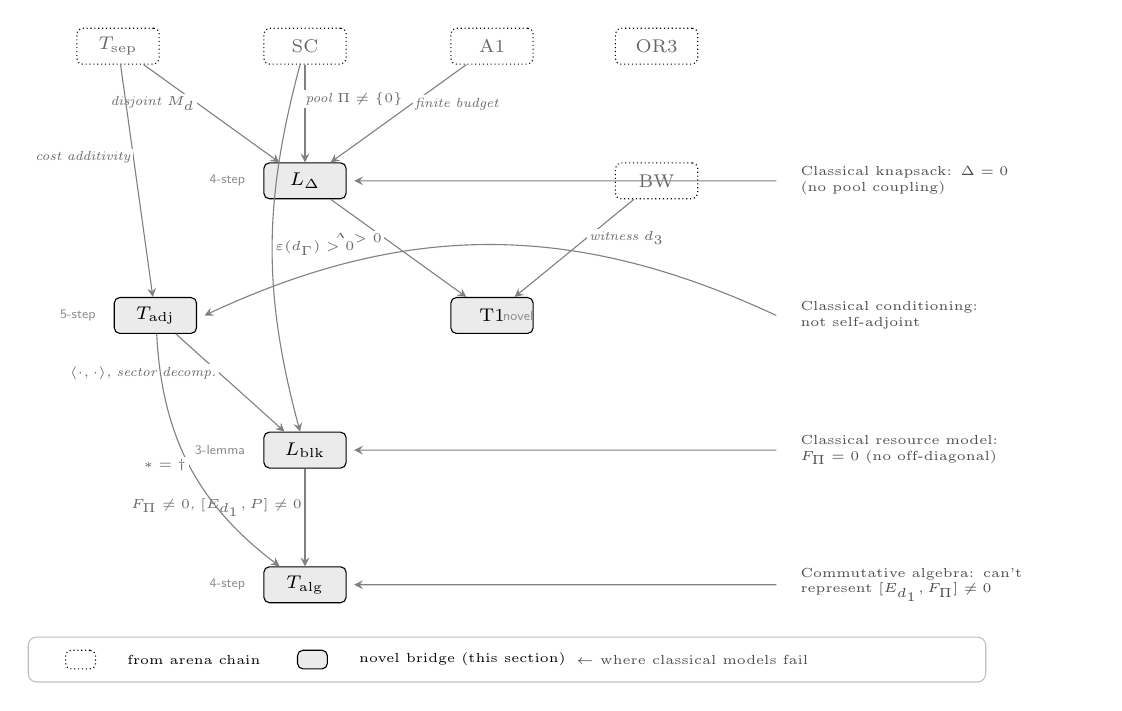
\begin{tikzpicture}[
    scale=0.95, every node/.style={transform shape},
    nd/.style={draw, rounded corners=2pt, minimum height=0.48cm, minimum width=1.1cm, inner sep=2pt, font=\scriptsize},
    prior/.style={nd, densely dotted, text=black!60},
    bridge/.style={nd, fill=black!8},
    lemma/.style={nd},
    arr/.style={->, >=stealth, thin, black!50},
    elabel/.style={font=\tiny\itshape, text=black!60, fill=white, inner sep=1pt},
    badge/.style={font=\tiny, text=black!45, anchor=east},
    cfail/.style={font=\tiny, text=black!70, anchor=west, text width=3.8cm, align=left},
]

\node[prior] (Tsep) at (-2.0, 0) {$T_{\mathrm{sep}}$};
\node[prior] (SC) at (0.5, 0) {SC};
\node[prior] (A1) at (3.0, 0) {A1};
\node[prior] (OR3) at (5.2, 0) {OR3};
\node[prior] (BW) at (5.2, -1.8) {BW};

\node[bridge] (LDelta) at (0.5, -1.8) {$L_\Delta$};
\node[bridge] (Tadj) at (-1.5, -3.6) {$T_{\mathrm{adj}}$};
\node[bridge] (T1) at (3.0, -3.6) {T1};
\node[bridge] (Lblk) at (0.5, -5.4) {$L_{\mathrm{blk}}$};
\node[bridge] (Talg) at (0.5, -7.2) {$T_{\mathrm{alg}}$};

\node[badge] at ($(LDelta.west)+(-0.12,0)$) {\textsf{4-step}};
\node[badge] at ($(Tadj.west)+(-0.12,0)$) {\textsf{5-step}};
\node[badge] at ($(T1.east)+(0.12,0)$) {\textsf{novel}};
\node[badge] at ($(Lblk.west)+(-0.12,0)$) {\textsf{3-lemma}};
\node[badge] at ($(Talg.west)+(-0.12,0)$) {\textsf{4-step}};

\draw[arr] (Tsep) -- node[elabel, left, pos=0.4] {disjoint $M_d$} (LDelta);
\draw[arr] (SC) -- node[elabel, right=-1pt, pos=0.35] {pool $\Pi \ne \{0\}$} (LDelta);
\draw[arr] (A1) -- node[elabel, right, pos=0.4] {finite budget} (LDelta);
\draw[arr] (Tsep) -- node[elabel, left, pos=0.4] {cost additivity} (Tadj);
\draw[arr] (LDelta) -- node[elabel, left, pos=0.4] {$\Delta > 0$} (T1);
\draw[arr] (BW) -- node[elabel, right, pos=0.4] {witness $d_3$} (T1);
\draw[arr] (Tadj) -- node[elabel, left, pos=0.4] {$\langle\cdot,\cdot\rangle$, sector decomp.} (Lblk);
\draw[arr] (SC) to[bend right=15] node[elabel, right, pos=0.5] {$\varepsilon(d_\Gamma) > 0$} (Lblk);
\draw[arr] (Lblk) -- node[elabel, left, pos=0.4] {$F_\Pi \ne 0$, $[E_{d_1},P]\ne 0$} (Talg);
\draw[arr] (Tadj) to[bend right=25] node[elabel, left, pos=0.5] {$* = \dagger$} (Talg);

\node[cfail] at (7.0, -1.8) {Classical knapsack: $\Delta = 0$\\(no pool coupling)};
\node[cfail] at (7.0, -3.6) {Classical conditioning:\\not self-adjoint};
\node[cfail] at (7.0, -5.4) {Classical resource model:\\$F_\Pi = 0$ (no off-diagonal)};
\node[cfail] at (7.0, -7.2) {Commutative algebra: can't\\represent $[E_{d_1}, F_\Pi] \ne 0$};

\draw[->, >=stealth, thin, black!50] (6.8, -1.8) -- ($(LDelta.east)+(0.1,0)$);
\draw[->, >=stealth, thin, black!50] (6.8, -3.6) to[bend right=25] ($(Tadj.east)+(0.1,0)$);
\draw[->, >=stealth, thin, black!50] (6.8, -5.4) -- ($(Lblk.east)+(0.1,0)$);
\draw[->, >=stealth, thin, black!50] (6.8, -7.2) -- ($(Talg.east)+(0.1,0)$);

\draw[black!25, rounded corners=3pt] (-3.2, -8.5) rectangle (9.6, -7.9);
\node[prior, minimum width=0.4cm, minimum height=0.25cm] at (-2.5, -8.2) {};
\node[font=\tiny, anchor=west] at (-2.0, -8.2) {from arena chain};
\node[bridge, minimum width=0.4cm, minimum height=0.25cm] at (0.6, -8.2) {};
\node[font=\tiny, anchor=west] at (1.1, -8.2) {novel bridge (this section)};
\node[font=\tiny, text=black!70, anchor=west] at (4.0, -8.2) {$\leftarrow$ where classical models fail};

\end{tikzpicture}
\caption[Bridge chain]{%
\textbf{Bridge chain: from superadditivity to noncommutativity (branch-(IJC) premise of the Sep/IJC Representation Theorem).}
Dotted nodes are arena-chain results; shaded nodes are novel.
Right annotations mark where each class of classical model fails.
The chain runs given the (IJC) premise of the Sep/IJC Representation Theorem; under (Sep) the algebra is automatically commutative and the bridge is vacuous (spectator countermodel correctly housed there).
}
\label{fig:bridge_dag}
\end{figure}

\begin{tcolorbox}[apfbox, title={The physical grounding: Stern--Gerlach and the order of enforcement}]
The chain $L_\Delta \to T_1 \to T_{\mathrm{adj}} \to L_{\mathrm{blk}} \to T_{\mathrm{alg}}$ is the heart of the bridge from finite capacity to quantum structure.  The conclusion --- that the enforcement algebra admits no faithful commutative representation --- can feel abstract.  Stern--Gerlach grounds it.

\smallskip\noindent A spin-$1/2$ particle is passed through a $z$-oriented Stern--Gerlach apparatus and filtered to spin-up in $z$.  That filtered beam is passed through an $x$-oriented apparatus and filtered to spin-up in $x$, then back through a $z$-apparatus.  The final $z$-apparatus shows both spin-up and spin-down outcomes, in equal numbers.  The intermediate $x$-filter has ``reset'' the $z$-distinction: what had been a pure $z$-up state no longer is.

\smallskip\noindent Read through the framework: enforcing the $z$-distinction, then the $x$-distinction, then the $z$-distinction again does not return to where enforcing $z$ alone leaves us.  The residual budget after $(z)$ differs from the residual after $(z, x, z)$.  That is $T_1$'s order-dependence, measured in the lab.  That the operators are self-adjoint is $T_{\mathrm{adj}}$: the cost of the $z$-then-$x$ sequence equals the cost of the $x$-then-$z$ sequence --- the enforcement budget is symmetric, differ only in their end-states.  That no commutative algebra represents them is $T_{\mathrm{alg}}$: the two sequences leave the system in states no classical conditional update can reach.

\smallskip\noindent Stern--Gerlach is the laboratory witness to the chain.  The mathematics of noncommutativity does the work; the experiment shows that the work is being done.
\end{tcolorbox}


% ======================================================================
\subsection{Preview: from noncommutative continuation structure to Hilbert representation (T2)}
\label{sec:T2}\label{sec:T2a}\label{sec:skeleton}\label{sec:T2c}

The enforcement algebra $\mathcal{A} = \mathrm{Alg}_\mathbb{R}(\mathcal{G}) \subseteq \mathrm{End}(V)$ (where $\mathcal{G} = \{E_d\} \cup \{E_{\{d_1,d_2\}}\}$) is a finite-dimensional real $*$-algebra with self-adjoint generators ($T_{\mathrm{adj}}$) and a faithful positive state $\omega(A) = \varepsilon(A)/C$.  Three steps convert it to a complex Hilbert-space representation.

\begin{tcolorbox}[apfbox, title={T2: Noncommutativity $\to$ Operator Algebra on Hilbert Space}]
\textit{The noncommutative enforcement algebra, via GNS and Wedderburn--Artin, becomes a $*$-subalgebra of $B(\mathcal{H})$ for a finite-dimensional complex Hilbert space $\mathcal{H}$.}

\smallskip\noindent\textbf{Statement.}  Under OR0--OR3, the enforcement algebra admits a faithful $*$-representation on a finite-dimensional complex Hilbert space: $\mathcal{A} \hookrightarrow B(\mathcal{H})$ with $\mathcal{A} \cong \bigoplus_k M_{n_k}(\mathbb{C})$.

\smallskip\noindent\textbf{T2a} (Real $*$-algebra).  The enforcement operations generate a finite-dimensional real $*$-algebra $\mathcal{A} \subseteq \mathrm{End}(V)$ with $\dim V \le n_{\max} + 1 < \infty$.  The GNS construction applied to $\omega$ yields a faithful $*$-representation $\pi_\omega: \mathcal{A} \hookrightarrow B(\mathcal{H}_\omega)$.  \textit{Key steps:} O1 (affine-to-linear extension), O3 (algebra closure under composition), O4 (positivity of $\omega$).

\smallskip\noindent\textbf{T2b} (Complexification + Wedderburn).  Complexify: $\mathcal{A}_\mathbb{C} = \mathcal{A} \otimes_\mathbb{R} \mathbb{C}$.  By Wedderburn--Artin (finite-dimensional semisimple algebras): $\mathcal{A}_\mathbb{C} \cong \bigoplus_k M_{n_k}(\mathbb{F}_k)$ with $\mathbb{F}_k \in \{\mathbb{R}, \mathbb{C}, \mathbb{H}\}$.

\smallskip\noindent\textbf{T2c} ($\mathbb{F} = \mathbb{C}$).  Two conditions select the complex branch: $P_{\mathrm{tom}}$ (local tomographic completeness, from $L_{\mathrm{loc}}$) eliminates $\mathbb{H}$; $P_{\mathrm{cls}}$ (closure under complex linear combinations of pure states, from A1's real-valued budget) eliminates $\mathbb{R}$.  Result: $\mathbb{F}_k = \mathbb{C}$ for all $k$, giving $\mathcal{A} \cong \bigoplus_k M_{n_k}(\mathbb{C}) \subseteq B(\mathcal{H})$.  \hfill$\square$

\smallskip\noindent Full proofs of T2a--T2c (including propositions O1--O4, T1b, and worked $M_2(\mathbb{C})$ verification) in Technical Supplement.  Anti-circularity audit (GNS, Wedderburn--Artin, Gleason/Busch, Skolem--Noether form a strictly acyclic dependency chain) also in Technical Supplement.

\coderef{check\_T2}{paper1.py}
\end{tcolorbox}

\smallskip\noindent The destination of Paper~1's own derivation chain is the noncommutative continuation structure of $T_{\mathrm{alg}}$ in \S\ref{sec:operator_bridge}. T2 is presented here as a \emph{preview} of where that structure leads when the standard representation-theoretic ascent is supplied: starting from PLEC's four constitutive features (A1 capacity bound + MD positive cost floor + A2 argmin selection + BW cost-spectrum non-degeneracy) on FD1's enforcement-interface triple $(S_\Gamma, \mathcal{D}(\Gamma), C(\Gamma))$ --- i.e., starting from \emph{admissibility space} per Paper~0 --- the bridge ($L_\Delta$, T1, $T_{\mathrm{adj}}$, $L_{\mathrm{blk}}$, $T_{\mathrm{alg}}$) delivers a noncommutative continuation algebra. The further ascent to a complex Hilbert representation requires additional representation, field-selection, and tensor hypotheses that are previewed below. Full formal development of the Hilbert-representation step --- of which T2 is the natural placeholder --- is deferred to the quantum-structure paper. The compressed reading remains accurate at the preview level: the quantum formalism is consistent with what minimum-cost finite enforcement of distinction looks like at (IJC) interfaces, and consequences such as the Born rule, Tsirelson-type bounds, gauge structure, and dynamics flow downstream from this construction once the additional hypotheses are supplied.

\begin{tcolorbox}[apfbox, title={Why exactly $\mathbb{C}$: the narrow selection by $T_{2c}$}]
Wedderburn--Artin gives three admissible fields for a finite-dimensional $*$-algebra: $\mathbb{R}$, $\mathbb{C}$, $\mathbb{H}$ (quaternions).  Each supports a matrix algebra structure; each, in principle, could carry a quantum-like theory.  That the framework selects $\mathbb{C}$ specifically --- not $\mathbb{R}$, not $\mathbb{H}$ --- is the content of $T_{2c}$.  Two exclusions do the work.

\smallskip\noindent\textbf{$\mathbb{R}$-exclusion} ($T_{2c.1}$).\quad Real amplitudes carry magnitude but not phase.  A real-amplitude theory can account for interference of intensities but not for interference of probability amplitudes; coherent superposition dissolves into incoherent mixing.  The closure premise $P_{\mathrm{cls}}$ --- closure under complex linear combinations of pure states, inherited from A1's real-valued budget and the GNS construction --- is what a real field cannot supply.

\smallskip\noindent\textbf{$\mathbb{H}$-exclusion} ($T_{2c.2}$).\quad Quaternion amplitudes supply phase, but too much: quaternion multiplication is non-commutative, so the order of contributions in a multi-path interference sum would itself be a physical quantity.  The tomographic premise $P_{\mathrm{tom}}$ --- local tomographic completeness, inherited from $L_{\mathrm{loc}}$'s locality of capacity --- forbids this extra structure at the local interface.  The quaternion degree of freedom has nowhere to live.

\smallskip\noindent The complex numbers are the unique admissible residue.  $\mathbb{C}$ carries phase (what $\mathbb{R}$ lacks) without importing a non-commutative multiplication on amplitudes (what $\mathbb{H}$ would force).  Neither too little nor too much: precisely the structure that the two premises carve out.

\smallskip\noindent\textbf{Physical anchor: the Aharonov--Bohm effect.}\quad An electron beam split around a solenoid and recombined picks up an interference phase proportional to the enclosed magnetic flux, even though the classical electromagnetic force on the electron along each path is zero.  The observed fringe shift $\psi \to e^{ie\Phi/\hbar}\,\psi$ is flatly incompatible with real amplitudes (which cannot encode a flux-dependent phase at all) and with quaternion amplitudes (which would predict path-order-dependent fringe patterns that experiments do not see).  The measured phase is complex-valued.  The laboratory selects $\mathbb{C}$; the framework derives that selection as $T_{2c}$.

\smallskip\noindent $T_{2c}$ is this selection, derived rather than assumed.  The complex field is not a mathematical convenience; it is the unique admissible amplitude structure under $P_{\mathrm{tom}} + P_{\mathrm{cls}}$.
\end{tcolorbox}

% ======================================================================
\subsection{Preview: \texorpdfstring{$T_{\mathrm{Born}}$}{T Born} --- Born probabilities from additional finite effect--state structure}

\noindent With the Hilbert-space representation in hand, the remaining results of quantum mechanics follow from standard theorems whose hypotheses T2 satisfies.  The Born rule is the first harvest: Gleason's theorem says that any probability measure on the projection lattice of a Hilbert space of dimension three or higher has the form $p = \mathrm{tr}(\rho P)$.  The enforcement framework satisfies Gleason's hypotheses because the enforcement cost is a finitely additive measure on the orthogonal projections produced by $T_{\mathrm{adj}}$.

\begin{tcolorbox}[apfbox, title={$T_{\mathrm{Born}}$: Born Rule from Admissibility Invariance}]
\textbf{Statement.}  On $\mathcal{H}$ from T2 with $\dim \mathcal{H} \ge 2$, the unique probability measure on projection-valued measurements is $p_i = \mathrm{tr}(\rho \cdot P_i)$.

\smallskip\noindent\textbf{Status.}  \textbf{[Standard: Gleason/Busch applied to T2's Hilbert space.]}  Conditional on T2.

\smallskip\noindent\textbf{Proof sketch.}  The enforcement measure $f(P) = \varepsilon(P)/C_{\mathrm{meas}}$ on the projection lattice $\mathcal{P}(\mathcal{H})$ satisfies: (NC) context-independence --- $f(P)$ depends only on $P$, not which PVM contains it (from $T_{\mathrm{sep}}$: cost depends only on anchor geometry); (OA) ortho-additivity --- $PQ = 0 \Rightarrow f(P+Q) = f(P) + f(Q)$ (from cost additivity on disjoint anchors).  NC + OA satisfy Gleason's frame-function hypothesis.  Route~B (primary): Busch's theorem~\cite{Busch2003} extends to $\dim = 2$ via GNS linearity.  Result: $f(P) = \mathrm{tr}(\rho P)$ for a unique density operator $\rho$.  \hfill$\square$

\coderef{check\_T\_Born}{paper1.py}
\end{tcolorbox}


% ======================================================================
\subsection{Preview: \texorpdfstring{$T_{\mathrm{Tsirelson}}$}{T Tsirelson} --- Tsirelson-type bounds after tensor / composition identification}
\label{sec:T_Tsirelson}

\noindent The CHSH inequality bounds how strongly correlated two spatially separated measurements can be.  Classical systems obey the Bell bound of~2; quantum mechanics permits up to $2\sqrt{2}$ but no more.  Remarkably, the enforcement framework derives this upper bound from the real $*$-algebra alone---before complexification, before the Born rule, before any Hilbert-space structure.  The bound is a consequence of finite enforcement, not of quantum mechanics per se.

\begin{tcolorbox}[apfbox, title={$T_{\mathrm{Tsirelson}}$: Tsirelson Bound $\le 2\sqrt{2}$}]
\textbf{Statement.}  For any CHSH operator $\hat{S} = a_1 \otimes (b_1 + b_2) + a_2 \otimes (b_1 - b_2)$ constructed from enforcement observables, $|\omega(\hat{S})| \le 2\sqrt{2}$.  Saturation at exactly $2\sqrt{2}$ is achievable.

\smallskip\noindent\textbf{Proof sketch.}  \textit{Step 1} (Tensor structure): $L_{\mathrm{loc}}$ gives $V_{AB} = V_A \otimes V_B$ for independent interfaces.  \textit{Step 2} (Dichotomic observables): binary predicates + $T_{\mathrm{adj}}$ give $a_i^2 = I$, $b_j^2 = I$ (self-adjoint unitaries).  \textit{Step 3} (Cirel'son identity): $\hat{S}^2 = 4I - [a_1,a_2] \otimes [b_1,b_2]$ (associative algebra only).  \textit{Step 4} (Norm bound): $\|[a,a']\|_{\mathrm{op}} \le 2$ by triangle inequality; hence $\|\hat{S}\|_{\mathrm{op}} \le 2\sqrt{2}$; state bound $|\omega(\hat{S})| \le \|\hat{S}\|$ by spectral theorem.  \textit{Saturation}: requires $\mathbb{F} = \mathbb{C}$ (T2c); the singlet state achieves $2\sqrt{2}$ with optimal observables $(\sigma_z \pm \sigma_x)/\sqrt{2}$.  \hfill$\square$

\smallskip\noindent\textit{Key structural point.}  The bound $\le 2\sqrt{2}$ is pre-Hilbert: it uses only the real $*$-algebra from T2a, the operator norm on $\mathrm{End}(V)$, and $L_{\mathrm{loc}}$'s tensor structure.  Only saturation requires T2c's complex field.

\coderef{check\_Tsirelson}{paper1.py}
\end{tcolorbox}

\section{Consequences, applications, and physical content}
\label{sec:consequences}
% ======================================================================

\noindent With the algebraic skeleton in hand, this section develops its consequences: an accessible walkthrough of the full argument (\S\ref{sec:walkthrough}), cost-functional applications (\S\ref{sec:cost_consequences}), an independent second route to the algebra via non-Boolean state cones (\S\ref{sec:T1NB_route}), conditional theorems and empirical predictions (\S\ref{sec:predictions}), and the canonical mathematical object forced by A1 (\S\ref{sec:canonical}).  Constructive $L_\Delta$ verifications, the detailed MD discussion, worked examples, and perturbation-lemma proofs are in the Technical Supplement.

\subsection{The argument: an accessible walkthrough}
\label{sec:walkthrough}\label{sec:argument}

\noindent\textit{This section gives a self-contained narrative of the complete
derivation from A1 to the Born rule.  Every claim is proved in
Sections~\ref{sec:defs}--\ref{sec:formal_bridge} and machine-verified in
\texttt{paper1.py}.}

\medskip

\noindent\textbf{Admissibility space and PLEC's four constitutive features.} Our bedrock is \emph{admissibility space} --- the FD1 enforcement-interface triple $(S_\Gamma, \mathcal{D}(\Gamma), C(\Gamma))$ at every causally-connected region (Paper~1 Supplement \S``Definitions (FD1--FD6)'', canonical bedrock) --- structured by PLEC's four constitutive features.  A distinction $d \in \mathcal{D}(\Gamma)$ is a binary partition on the substrate $S_\Gamma$ maintained against perturbation at cost $\varepsilon(d) > 0$.  PLEC's four features:  \textbf{A1} (capacity bound) gives $\sum_d \varepsilon(d) \le C(\Gamma) < \infty$; \textbf{MD} (positive cost floor) gives $\varepsilon(d) \ge \mu^* \cdot n(d) > 0$; \textbf{A2} ($\arg\min$ selection) gives the realised configuration as $\arg\min$ of $\sum \varepsilon$ over the admissible set; \textbf{BW} (cost-spectrum non-degeneracy) ensures a budget-window triple exists.  These four are pairwise structurally independent (Technical Supplement \S1 essentiality proofs).

\medskip
\noindent\textbf{A finite arena.}  MD gives $\varepsilon^* > 0$ [$L_{\varepsilon^*}$].  Combined with A1's finite budget, at most $n_{\max} = \lfloor C/\varepsilon^* \rfloor$ distinctions can be active simultaneously, so the substrate $S_\Gamma$ is finite-dimensional [$T_{\mathrm{form}}$, $T_{\mathrm{embed}}$].

\medskip
\noindent\textbf{Separation and the pool.}  Distinctions with disjoint anchor sets have additive costs [$T_{\mathrm{sep}}$].  When two distinctions share an interface, the pool $\Pi := S_\Gamma \setminus (M_{d_1} \oplus M_{d_2})$ carries a substrate-integrity distinction $d_\Gamma$ with $\varepsilon(d_\Gamma) > 0$ (by A1).  By $T_{\mathrm{sep}}$ applied to pairwise-disjoint anchors: $\varepsilon(\{d_1, d_2\}) = \varepsilon(d_1) + \varepsilon(d_2) + \Delta$ with $\Delta = \varepsilon(d_\Gamma) > 0$.  This is $L_\Delta$: co-located distinctions cost strictly more together than apart.

\medskip
\noindent\textbf{Order-dependence (T1).}  With $\Delta > 0$, the residual budgets after enforcing $d_1$ alone versus $d_2$ alone differ when $\varepsilon(d_1) \ne \varepsilon(d_2)$ (NT).  BW supplies a witness $d_3$ in the budget window that is admissible after one ordering but not the other: enforcement is order-dependent.

\medskip
\noindent\textbf{Three steps to noncommutativity.}  (1)~$T_{\mathrm{adj}}$: cost symmetry forces a sector-orthogonal bilinear form, making enforcement projections self-adjoint.  (2)~$L_{\mathrm{blk}}$: since $\Delta > 0$, no direct-sum-realizable defender exists; the remainder $F_\Pi \ne 0$ is forced.  (3)~$T_{\mathrm{alg}}$: $[E_{d_1}, F_\Pi] = -\pi_v \ne 0$; no faithful commutative $*$-representation exists.

\medskip
\noindent\textbf{From algebra to Hilbert space.}  T2a (semisimplicity via Jacobson radical), $T_{\mathrm{GNS}}$ (faithful $*$-representation on $\mathcal{H}_\omega$), T2b (Wedderburn--Artin: $\mathcal{A} \cong \bigoplus_k M_{n_k}(\mathbb{F}_k)$), T2c (field selection $\mathbb{F} = \mathbb{C}$ via parameter count, $P_{\mathrm{tom}}$, $P_{\mathrm{cls}}$).  $T_{\mathrm{Born}}$: Busch's generalized Gleason theorem gives $\mathrm{Prob}(d \mid \sigma) = \mathrm{tr}(\rho_\sigma E_d)$.

\medskip
\noindent The end-to-end chain is:
\begin{equation}\label{eq:arg_chain}
\underbrace{\text{A1}}_{\text{axiom}} \;\to\;
\underbrace{L_\Delta}_{\Delta > 0} \;\to\;
\underbrace{\text{T1}}_{\text{order-dep.}} \;\to\;
\underbrace{T_{\mathrm{adj}}}_{E_d = E_d^\dagger} \;\to\;
\underbrace{L_{\mathrm{blk}}}_{F_\Pi \ne 0} \;\to\;
\underbrace{T_{\mathrm{alg}}}_{[E,F]\ne 0} \;\to\;
\underbrace{T_{\mathrm{GNS}}}_{\mathcal{H}} \;\to\;
\underbrace{\text{T2c}}_{\mathbb{C}} \;\to\;
\underbrace{T_{\mathrm{Born}}}_{\mathrm{Born\;rule}}.
\end{equation}

\medskip
\noindent\textbf{What is novel, what is standard.}  The novel segment is $L_\Delta \to L_{\mathrm{blk}} \to T_{\mathrm{alg}}$: positive excess cost equivalent to failure of direct-sum realizability, and the three-line commutator witness.  The standard segment is $T_{\mathrm{embed}}$, $T_{\mathrm{GNS}}$, T2c (known theorems applied to enforcement data).

\smallskip
\noindent\textbf{Proof map.}

\smallskip
\begin{center}
\captionof{table}{Proof map: where each argument step is verified.}
\label{tab:proof_map}
\smallskip
\renewcommand{\arraystretch}{1.3}
\small
\begin{tabular*}{\textwidth}{@{\extracolsep{\fill}}llll@{}}
\textbf{Step} & \textbf{Result} & \textbf{Location} & \textbf{What to look for} \\[2pt]
\hline\noalign{\smallskip}
Finite arena & $L_{\varepsilon^*}$, $T_{\mathrm{form}}$ & \S\ref{sec:logical_status_eps_star}, \ref{sec:defs} & Cost-floor proof; counting bound $n_{\max} = \lfloor C/\varepsilon^*\rfloor$ \\[3pt]
Cost additivity & $T_{\mathrm{sep}}$ & \S\ref{sec:defs} & Biconditional, each $\sim$5 lines \\[3pt]
Superadditivity & $L_\Delta$ & \S\ref{sec:L_Delta} & Substrate-integrity derivation \\[3pt]
Order-dependence & T1 & \S\ref{sec:L_Delta} & Three-operation witness \\[3pt]
Self-adjointness & $T_{\mathrm{adj}}$ & \S\ref{sec:operator_bridge} & Five-step proof in named box \\[3pt]
$\oplus$-Failure & $L_{\mathrm{blk}}$ & \S\ref{sec:operator_bridge} & $\Delta > 0 \Leftrightarrow$ no block-diag.\ defender \\[3pt]
Noncommutativity & $T_{\mathrm{alg}}$ & \S\ref{sec:operator_bridge} & Commutator witness + faithfulness \\[3pt]
Hilbert space & $T_{\mathrm{GNS}}$, T2c & \S\ref{sec:T2} & GNS + Wedderburn--Artin + field selection \\[3pt]
Born rule & $T_{\mathrm{Born}}$ & \S\ref{sec:T2} & Busch's theorem \\[3pt]
\end{tabular*}
\end{center}

\smallskip\noindent The codebase is publicly available at
\url{https://github.com/Ethan-Brooke/APF-Paper-1-The-Enforceability-of-Distinction}.
All theorem boxes carry a \textit{Code reference:} tag pointing to
\texttt{paper1.py} (82 checks) or additionally to \texttt{supplement.py} (44 checks).

\smallskip\noindent A complete finite worked example ($C = 5$, three distinctions, explicit $L_\Delta$ verification, P1--P4 checks, order-dependent witness, and commutative-algebra obstruction) is given in Part~II of the Technical Supplement.\label{sec:worked_example}


\subsection{Cost functional: physical applications}
\label{sec:cost_consequences}

\noindent $L_{\mathrm{cost}}$ (Section~\ref{sec:L_cost}) establishes that any quantity $\varphi$ satisfying positivity (V1), vanishing (V2), and additive independence (V3) has the unique form $\varphi(E) = n(E) \cdot \varphi(1)$, where $n(E) \in \mathbb{N}$ is the integer channel count.  This is a proportionality theorem: any two qualifying proxies are proportional, with a domain-specific conversion factor.  Full scope delimitation (V1--V3 criteria, necessity argument, worked QEC verification, and dual-ruler end-to-end test in the Kitaev toric code) is in the Technical Supplement.\label{sec:Lcost_worked}\label{sec:dual_ruler}\label{box:Lcost_proportionality}

\smallskip
\begin{center}
\captionof{table}{Verification of $L_{\mathrm{cost}}$ conditions for three physical proxies.}
\smallskip
{\small
\begin{tabular*}{\textwidth}{@{\extracolsep{\fill}}llll@{}}
\textbf{Quantity} & \textbf{Positive?} & \textbf{Zero (trivial)?} & \textbf{Additive (indep.)?} \\[2pt]
\hline\noalign{\smallskip}
Energy gap $\Delta E$ & $\Delta E > 0$ & $\Delta E = 0$ (vacuum) & Yes (indep.\ modes) \\[3pt]
QEC overhead $\gamma$ & $\gamma > 0$ & $\gamma = 0$ (no code) & Yes (indep.\ stabilizers) \\[3pt]
BH entropy $S_{\mathrm{BH}}$ & $S > 0$ for $A > 0$ & $S = 0$ for $A = 0$ & Yes (disjoint horizons) \\
\end{tabular*}}
\label{tab:physical_proxies}
\end{center}

\smallskip\noindent Each satisfies V1--V3.  By $L_{\mathrm{cost}}$, each is provably proportional to $\varepsilon(E)$ with a conversion factor: $\Delta E = \alpha_E \cdot \varepsilon$, $\gamma = \alpha_\gamma \cdot \varepsilon$, $S_{\mathrm{BH}} = \alpha_S \cdot \varepsilon$.  All structural predictions depend only on dimensionless ratios $\varepsilon(d)/C = n(d)/n_{\max}$, from which every conversion factor cancels.


\subsection{Second route: non-Boolean state cone (Proposition T1-NB)}
\label{sec:T1NB_route}\label{sec:T1NB}

\noindent The derivation chain A1 $\to$ $L_\Delta$ $\to$ T1 $\to$ $T_{\mathrm{adj}}$ $\to$ $T_{\mathrm{alg}}$ $\to$ T2 is the primary route to Hilbert space.  But a single chain, however rigorous, invites the question: does the conclusion depend on some artefact of the particular path?  The following result answers that question by providing a completely independent second route to the same algebra, sharing only $L_\Delta$ and $T_{\mathrm{adj}}$ as common input.

\begin{tcolorbox}[apfbox, title={Proposition T1-NB (Non-Boolean Bridge)}]
\textit{Superadditivity forces a non-Boolean effect algebra; the state cone is not a simplex; finite-dimensionality + self-duality + irreducibility force a symmetric cone; Koecher--Vinberg identifies a Euclidean Jordan algebra; Albert classification + field selection gives $\bigoplus_k M_{n_k}(\mathbb{C})$.}

\smallskip\noindent\textbf{Statement.}  Under the premises $L_\Delta$, $L_{\mathrm{loc}}$, OR1, $T_{\mathrm{adj}}$, OR3, the enforcement algebra is isomorphic to a direct sum of full complex matrix algebras.

\smallskip\noindent\textbf{Proof sketch (six steps).}  (1)~$L_\Delta$'s superadditive valuation violates Boolean additivity $\Rightarrow$ $\mathcal{E}$ not Boolean.  (2)~Non-Boolean + $T_{\mathrm{adj}}$'s inner product $\Rightarrow$ self-dual cone $K = K^*$ (finite-dimensional argument, no GNS).  (3)~$L_{\mathrm{loc}}$ $\Rightarrow$ $K$ irreducible (Cartesian factors would give $\Delta = 0$).  (4)~Vinberg: finite-dimensional irreducible self-dual $\Rightarrow$ symmetric.  (5)~Koecher--Vinberg: symmetric cone $\Rightarrow$ EJA.  (6)~Albert classification + $P_{\mathrm{tom}}$ (excludes $\mathbb{R}$) + $P_{\mathrm{cls}}$ (excludes $\mathbb{H}$) + $L_{\mathrm{loc}}$ (excludes Albert algebra and non-factorizable spin factors) $\Rightarrow$ $\mathcal{A} \cong \bigoplus_k M_{n_k}(\mathbb{C})$.  Full proof in Technical Supplement.  \hfill$\square$
\end{tcolorbox}

\smallskip\noindent\textbf{Two-route convergence.}  Route~A ($L_{\mathrm{blk}} \to T_{\mathrm{alg}}$) and Route~B ($L_\Delta \to$ Choquet $\to$ Vinberg $\to$ Albert) share only $L_\Delta$ and $T_{\mathrm{adj}}$ as input.  Route~A never mentions simplices or Jordan algebras; Route~B never mentions direct-sum realizability.  The algebra is doubly derived.


\subsection{Conditional theorems, regime transitions, and empirical predictions}
\label{sec:predictions}

\noindent The following results follow from T2 given explicitly stated identifications between enforcement quantities and standard quantum-mechanical objects.

\begin{tcolorbox}[apfbox, title={Conditional Theorems: $P_{\mathrm{coll}}$, $T_{\mathrm{CPTP}}$, $T_{\mathrm{tensor}}$, $T_{\mathrm{entropy}}$, $T_M$}]
\label{sec:collision_model}
\textbf{$P_{\mathrm{coll}}$ (Collision Model).}  Sequential enforcement acts have collision-model structure: each step is a unitary interaction with a fresh ancilla drawn from the substrate pool.  \textbf{[Proved]} from $T_{\mathrm{sep}}$ + T2 + $L_{\varepsilon^*}$.  Seeds the dynamics programme of Paper~3.

\smallskip\noindent\textbf{$T_{\mathrm{CPTP}}$ (Admissible Dynamics).}  Budget-preserving enforcement maps are CPTP.  \textbf{[Conditional on identification \#2; full proof Paper~3.]}

\smallskip\noindent\textbf{$T_{\mathrm{tensor}}$ (Tensor Products).}  Independent-budget interfaces compose via $\mathcal{H}_A \otimes \mathcal{H}_B$.  \textbf{[Conditional on identification \#3.]}

\smallskip\noindent\textbf{$T_{\mathrm{entropy}}$ (Von Neumann Entropy).}  $S(\omega) = -\mathrm{tr}(\rho\log\rho)$ equals committed capacity fraction.  Wehrl--Uhlmann hypotheses verified from T2 + $L_{\mathrm{loc}}$ + OR1.  \textbf{[Conditional on $T_{\mathrm{tensor}}$.]}

\smallskip\noindent\textbf{$T_M$ (Interface Monogamy).}  No single interface can be simultaneously maximally entangled with two independent partners.  \textbf{[Proved]} from $T_{\mathrm{tensor}}$ + Araki--Lieb + $L_{\mathrm{loc}}$.
\end{tcolorbox}


\subsubsection*{Regime transitions and empirical predictions}
\label{sec:regime_models_full}\label{box:regime_experimental}\label{box:operationalize_r}

\noindent Two exact regime boundaries emerge from the minimal two-distinction model.  The control parameter is $r := C/\varepsilon^*$.  The \textbf{decoherence onset} at $r = 4$ marks the threshold below which the budget cannot sustain coherent joint enforcement.  The \textbf{enforcement-exclusion boundary} at $r = 1$ marks the threshold at which no second distinction can anchor.  Both are parameter-free; derivations from $L_\Delta$, $T_M$, and T2 are in the Technical Supplement.

\medskip\noindent\textbf{Crossover formula.}\label{box:experimental_protocol}  Defining $x := S(\omega_0)/S_{\mathrm{th}} - 1$ (reduced excess spectral weight), the APF prediction near threshold is:
\begin{equation}\label{eq:crossover}
T_2^{-1}(x) \;=\; T_{2,\mathrm{bg}}^{-1} \;+\; \Gamma_{\mathrm{dec}}\, \max(x,\, 0)^{\mu(s)},
\end{equation}
where the crossover exponent $\mu(s)$ depends on the spectral index $s$ (sub-Ohmic $s < 1$: steepest kink; Ohmic $s = 1$: canonical kink; super-Ohmic $s > 1$: rounded crossover).  Standard Bloch--Redfield predicts monotone $T_2^{-1} \propto S(\omega_0)$ with no kink.  The discriminating observable is $d\ln T_2/d\ln S(\omega_0)$: a step from $0$ to $-1$ (APF) versus flat $-1$ (null).

\smallskip\noindent\textbf{Mode-count collapse.}  As the number of environmental modes $N_E$ increases, the threshold descends as $S_{\mathrm{th}}/N_E$ and the kink collapses toward the origin.  The spectral-index relation $\mu = s$ is a parameter-free falsifiable prediction.

\smallskip\noindent\textbf{Experimental platforms.}  Protocol~A (superconducting transmon with single near-resonant TLS) and Protocol~B (trapped ion with engineered phonon reservoir, $N_E = 1, 2, 4, 8$) are detailed in the Technical Supplement, including an IBM Eagle-class worked prediction ($r \approx 16$, $S_{\mathrm{th}} \approx 6 \times 10^{-14}\;\mathrm{rad}^2/\mathrm{Hz}$, detectable at $4.5\sigma$ in a single cooldown).


\subsection{The canonical object: what A1 uniquely admits}
\label{sec:canonical}

\noindent We began the paper by asking what physics permits: given a finite enforcement budget, what structure must any admissible system have?  T2 answered that it must be described by a complex Hilbert-space algebra.  The next result sharpens this to a unique object: the canonical enforcement structure is a von Neumann algebra with a gauge group, a faithful trace, a von Neumann entropy, and a spectrum of conditional theorems---all determined by A1 alone, with no free parameters.

\begin{tcolorbox}[apfbox, title={$T_{\mathrm{canonical}}$: The Canonical Object Forced by A1}]
\textbf{Statement.}  Within the operational, regularity, and representation framework fixed in this paper, A1 forces a unique mathematical skeleton:
\begin{equation}
\mathcal{A}(C, \varepsilon^*, \kappa) \;=\; \Bigl(\;\mathcal{H},\;\; \mathcal{A} \subset B(\mathcal{H}),\;\; G_{\mathrm{gauge}},\;\; S[\rho]\;\Bigr)
\end{equation}

\smallskip\noindent\textit{Components:}
\begin{varlist}
\item $\mathcal{H}$ --- finite-dimensional Hilbert space. \textit{Via:} A1 $\to$ $L_{\varepsilon^*}$ $\to$ $L_{\mathrm{nc}}$ $\to$ T1 $\to$ T2 (GNS).
\item $\mathcal{A} \subset B(\mathcal{H})$ --- C$^*$-algebra of observables. \textit{Via:} T2 (Wedderburn--Artin).
\item $G_{\mathrm{gauge}}$ --- compact gauge group. \textit{Via:} $L_{\mathrm{loc}}$ $\to$ T3 (Skolem--Noether + Tannaka--Krein).
\item $S[\rho] = -\mathrm{tr}(\rho \ln \rho)$ --- entropy functional. \textit{Via:} T2 $\to$ $T_{\mathrm{entropy}}$ (Schumacher compression).
\end{varlist}

\smallskip
The specific content --- $C_{\mathrm{total}} = 61$, $G_{\mathrm{gauge}} = SU(3) \times SU(2) \times U(1)$, numerical predictions --- is determined in Papers~2--7.

\coderef{check\_T\_canonical}{paper1.py}
\end{tcolorbox}


\medskip\noindent\textit{Empirical Content of Paper~1.}
\label{box:empirical_content}

\medskip\noindent\textbf{Category 1: Recovered known results} (consistency checks).

\begin{center}
\captionof{table}{Recovered known results from the enforcement framework.}
\label{tab:empirical_cat1}
\smallskip
\begin{tabular*}{\textwidth}{@{\extracolsep{\fill}}lll@{}}
\textbf{Result} & \textbf{Known value} & \textbf{APF derivation} \\[2pt]
\hline\noalign{\smallskip}
Tsirelson bound & $2\sqrt{2} \approx 2.828$ & T2 + Cirel'son identity ($T_{\mathrm{Tsirelson}}$) \\[3pt]
Born rule & $p_i = \mathrm{tr}(\rho P_i)$ & T2 + Busch/Gleason ($T_{\mathrm{Born}}$) \\[3pt]
No-broadcasting & Barnum et al.\ 1996 & T2 + T1 ($T_{\mathrm{NB}}$) \\[3pt]
No-signaling & Standard QM & $L_{\mathrm{loc}}$ ($T_{\mathrm{NS}}$) \\[3pt]
Field $= \mathbb{C}$ & Standard QM & T2c (param.\ count + $P_{\mathrm{tom}}$) \\
\end{tabular*}
\end{center}

\smallskip\noindent These are necessary consistency conditions, not predictions.

\medskip\noindent\textbf{Category 2: Novel predictions testable without $\varepsilon^*$ calibration.}  (a)~The decoherence kink (Eq.~\eqref{eq:crossover}).  (b)~Mode-count collapse of the kink ($S_{\mathrm{th}} \to S_{\mathrm{th}}/N_E$).  (c)~Spectral-index relation $\mu = s$.  (d)~Structural no-go: $r < 4$ excludes coherent joint enforcement.  No other quantum reconstruction program makes predictions (a)--(c).

\medskip\noindent\textbf{Category 3: Results requiring $\varepsilon^*$ calibration.}  Absolute threshold $S_{\mathrm{th}}$ in SI units, decoherence time $t_{\mathrm{dec}}$ from leakage, and capacity-wall onset --- all require identifying $\varepsilon^*$ in physical units (Paper~6: $\varepsilon^* = \alpha\ell_P^2$).
\label{tab:empirical_cat3}

\smallskip\noindent\textbf{Detailed MD discussion.}\label{sec:MD_detail}  The extended analysis of MD --- including the ``smuggling'' charge, the bootstrap argument (cost before geometry), countermodel analysis, near-equivalence with finite-dimensionality, and the Markov quiet regime equivalence (MD-eq) --- is in the Technical Supplement.

% Labels anchoring supplement cross-references
\label{sec:Ldelta_verifications}\label{sec:LP_verification}\label{sec:witnesses}\label{sec:toy_kappa}\label{sec:qskel}\label{tab:bridge_generators}\label{tab:bridge_steps}\label{sec:overlap_detail}\label{box:overlap_example}\label{sec:P1P4_detail}\label{sec:examples}\label{box:MD_operational}\label{box:MD_deep}

\section{Scope: what this paper derives and what it does not}
\label{sec:scope}
% ======================================================================

\subsection{What this paper establishes: precise scope}
\label{sec:precise_scope}

The following table gives the precise status of every result claimed in this
paper.  The distinction between ``proved here,'' ``conditional on stated
identifications,'' and ``deferred'' is maintained throughout.  The derivation of every piece of linear geometry from resource axioms is traced in the Linear Structure Provenance table (Technical Supplement); an independent categorical route to the same algebra via sequential effect algebras is given in Appendix~\ref{app:sea}.

\begin{center}
\small
\captionof{table}{Precise scope of Paper~1: status of every claimed result.  ``Proved here'' = full derivation in this paper with all hypotheses stated.  ``Conditional'' = derivation complete given a stated identification.  ``Deferred'' = opening result of the named companion paper.}
\smallskip
{\footnotesize
\begin{tabular*}{\textwidth}{@{\extracolsep{\fill}}lll@{}}
\toprule
\textbf{Result} & \textbf{Status} & \textbf{Depends on} \\
\midrule
A1 (Finite Enf.\ Capacity) & Physical axiom & --- \\
OR1 (Convex mixing) & \textbf{Derived} & A1 (real-valued budget) \\
$T_{\mathrm{adj}}$ (Self-adjointness) & \textbf{Proved here} & $T_{\mathrm{sep}}$ + cost additivity \\
$L_{\mathrm{atf}}$ (Active Threshold) & \textbf{Proved here} & A1 + defn.\ of $\mathcal{D}$ \\
Cost-Discreteness ($\varepsilon^*\!>\!0$) & Proved (MD $\to$ $L_{\varepsilon^*}$) & MD; OR3 from A1+MD+SC \\
Richness ($R_{\mathrm{loc}}$, $R$) & Declared & Physical content P2 \\
\midrule
$L_{\varepsilon^*}$, $L_{\mathrm{loc}}$, $L_{\mathrm{nc}}$, $L_\Delta$, $L_{\mathrm{irr}}$ & \textbf{Proved here} & A1 + stated premises \\
T1: Order dependence & \textbf{Proved here} & $L_\Delta$, NT, OR0, BW \\
T2a: Real $*$-algebra & \textbf{Proved here} & T1, O1--O4, OR0--OR3 \\
O1: Affine extension & Structural & OR1, OR3, $L_{\varepsilon^*}$ \\
T2b: Complex.\ + W--A & \textbf{Proved here} & T2a \\
T2c: $\mathbb{F}\!=\!\mathbb{C}$ & \textbf{Conditional} & T2b + $P_{\mathrm{tom}}$ + $P_{\mathrm{cls}}$ \\
T2: Hilbert space & \textbf{T2a+b uncond.; T2c cond.} & See T2a--T2c above \\
\midrule
$T_M$ (Monogamy) & \textbf{Proved here} & A1, $L_{\mathrm{loc}}$, $L_\Delta$ \\
$T_{\mathrm{NS}}$ (No-Signaling) & \textbf{Proved here} & $L_{\mathrm{loc}}$, $T_{\mathrm{tensor}}$ \\
$T_{\mathrm{NB}}$ (No-Broadcasting) & \textbf{Proved here} & T2, $T_{\mathrm{tensor}}$, $T_M$ \\
$T_{\mathrm{Born}}$: Born rule & \textbf{Conditional} & T2 + state id. \\
$T_{\mathrm{Herm}}$: self-adj.\ obs. & \textbf{Conditional} & T2 + real-valued costs \\
$T_{\mathrm{CPTP}}$: dynamics & \textbf{Conditional} & T2 + Stinespring + dyn.\ id. \\
$T_{\mathrm{tensor}}$: tensor prod. & \textbf{Conditional} & T2 + $L_{\mathrm{loc}}$ + dbl.\ comm.\ id. \\
T3: gauge skeleton & \textbf{Conditional} & T2 + Skolem--Noether \\
$T_{\mathrm{Tsi}}$: CHSH bound & \textbf{Conditional} & T2 + $T_{\mathrm{tensor}}$ \\
$T_{\mathrm{ent}}$: vN entropy & \textbf{Conditional} & T2 + capacity id. \\
\midrule
Gauge group, spectrum & Specified & Paper~2 \\
Three generations & Specified & Papers~3--4A \\
Spacetime, cosmo.\ params. & Specified & Papers~5--7 \\
\bottomrule
\end{tabular*}}
\label{tab:scope}
\end{center}

\smallskip\noindent\textbf{Scope of finite-dimensionality: per-interface at finite capacity, not universal.}
The finite-dimensional Hilbert space $\mathcal{H}_\omega$ with $\dim \le \lfloor C/\varepsilon^* \rfloor^2$ is derived for a single interface $\Gamma$ with finite capacity.  QFT's infinite-dimensional algebras correspond to the continuum limit $C \to \infty$; any experiment with finite energy, volume, and precision accesses only finitely many degrees of freedom, so OR3 is satisfied operationally.  The Bekenstein--Hawking bound confirms OR3 for bounded regions.


\smallskip\noindent\textbf{Precise status of $T_M$, $T_{\mathrm{NB}}$, and $T_{\mathrm{CPTP}}$.}
$T_M$ is proved unconditionally (A1 $\to$ $L_{\mathrm{loc}}$ $\to$ $L_\Delta$ $\to$ $T_M$); $T_{\mathrm{NB}}$ is proved unconditionally via the resource-budget route (Step~1) and additionally via the algebraic route conditional on the tensor identification; $T_{\mathrm{CPTP}}$ is conditional, with the structural architecture (collision-model $P_{\mathrm{coll}}$, trace preservation) proved here and the remaining continuity condition deferred to Paper~3.  Details of each proof-status tier are in the Technical Supplement.


\smallskip\noindent\textit{On ``conditional'' results in general.}  Results marked conditional are established given T2 and the stated identifications, using standard mathematical theorems (Gleason, Stinespring, double commutant, Skolem--Noether, Cirel'son identity) whose hypotheses T2 satisfies.  The required identifications are listed in Section~\ref{sec:identifications}.  They are not additional axioms of the framework; they are the operational meanings assigned to the Hilbert-space objects produced by T2.  A result is ``proved here'' if it follows from A1 and stated premises without any representation-level identification; it is ``conditional'' if it requires an identification to connect an enforcement quantity to a Hilbert-space object.

\smallskip\noindent\textbf{Specified in later papers.}
\label{sec:deferred}

The specific gauge group $SU(3)\times SU(2)\times U(1)$, particle content, mass hierarchies, mixing matrices, spacetime dimension and signature, cosmological constants, and quantitative predictions are all specified in Papers~2--7 by deploying the algebraic skeleton established here through specific budget channels.  None requires additional physical axioms; each is a specification of the richness premise R and the budget deployment --- analogous to specifying the initial conditions of a dynamical system whose equations of motion are already derived.  Full logical dependencies are traced in those papers.

\subsection{Complete assumption inventory}
\label{sec:assumption_inventory}


\medskip\noindent\textit{Assumption Inventory: What the Chain A1 $\to$ $L_\Delta$ $\to$ T1 $\to$ T2 Actually Requires.}
\label{box:assumption_inventory}

The critical path from A1 to T2 (Hilbert-space representation) requires exactly:

\medskip
\begin{center}
\captionof{table}{Critical-path inputs from A1 to T2 (Hilbert-space representation).}
\smallskip
{\small
\begin{tabular*}{\textwidth}{@{\extracolsep{\fill}}lll@{}}
\textbf{Input} & \textbf{Type} & \textbf{Content and status} \\[2pt]
\hline\noalign{\smallskip}
\textbf{A1} & Axiom & Enforcement capacity finite and positive.  Sole physical axiom. \\[4pt]
\textbf{MD} & Structural assum. & Enf.\ Isotropy: $\varepsilon(d) \ge \mu^* n(d)$.  Confirmed by BH bound (P6). \\[4pt]
\textbf{BW} & Richness premise & Budget-window triple with $d_3$ fitting $d_1$ not $d_2$.  Enters at T1 only. \\
\end{tabular*}}
\label{tab:critical_path}
\end{center}

\medskip\noindent\textbf{Everything else is derived:}

\smallskip
\begin{center}
\captionof{table}{Derived definitions and conditions (not independent inputs).}
\smallskip
{\small
\begin{tabular*}{\textwidth}{@{\extracolsep{\fill}}ll@{}}
FD1 (substrate) & FD1a primitive; FD1b derived from A1 + OR1 + $L_{\varepsilon^*}$ \\[2pt]
FD4 (cost) & Constitutive expression of A1 in FD1b + FD3 \\[2pt]
FD6 (joint defense) & Rotated codespace from $L_\Delta$ + optimization ($L_\Pi$, Tech.\ Suppl.) \\[2pt]
K1--K4 & All derived from A1 + OR3 \\[2pt]
SC & Derived from MD + $\mathcal{D}$-quotient \\[2pt]
OR1 & Derived from real-valued $C(\Gamma)$ \\[2pt]
$T_{\mathrm{adj}}$ & Proved from $T_{\mathrm{sep}}$ + cost additivity \\[2pt]
OR3 & Proved as $T_{\mathrm{form}}$ from A1 + MD + SC \\[2pt]
$L_{\mathrm{loc}}$ & Not on critical path; needed for $L_{\mathrm{irr}}$ and gauge branch \\[2pt]
$R_{\mathrm{loc}}$ & Not on critical path; needed for $L_{\mathrm{irr}}$ only \\
\end{tabular*}}
\label{tab:derived_items}
\end{center}

\medskip\noindent\textbf{Comparison with peer reconstruction programs:}

\smallskip
\begin{center}
\captionof{table}{Comparison with peer reconstruction programs: named input count.}
\smallskip
{\small
\begin{tabular*}{\textwidth}{@{\extracolsep{\fill}}lcl@{}}
\textbf{Program} & \textbf{Inputs} & \textbf{What APF derives instead} \\[2pt]
\hline\noalign{\smallskip}
Hardy (2001) & 5 axioms & Subspace axiom, simplicity \\
CDP (2011) & 6 axioms & Purification, local distinguishability \\
Masanes--M\"uller (2011) & 5 axioms & Cont.\ reversibility, tomographic locality \\
\textbf{APF (this paper)} & \textbf{A1+MD+BW} & OR1, $T_{\mathrm{adj}}$, OR3, $P_{\mathrm{tom}}$, $P_{\mathrm{cls}}$ proved \\
\end{tabular*}}
\label{tab:peer_comparison}
\end{center}

\smallskip\noindent The APF's total input count (1 axiom + 1 structural assumption + 1 richness premise = 3) is comparable to the above.  The trade-off: the definitional layer (FD1--FD6) is richer, but every item is now either constitutive or derived.



\subsection{Explicit identifications used in this paper}
\label{sec:identifications}

Four identifications connect enforcement-framework constructs to standard quantum objects.  Each is stated explicitly; results that require them are flagged as conditional.

\begin{enumerate}[nosep,leftmargin=2em,itemsep=4pt]
\item \textbf{State identification}: $\omega(A) = \mathrm{tr}(\rho\,\pi_\omega(A))$ — the GNS state functional corresponds to a density operator.
\item \textbf{Observable identification}: self-adjoint elements of $\mathcal{A}$ in the GNS representation correspond to quantum observables.
\item \textbf{Composition identification}: budget-independent interfaces compose via tensor product (used in $T_{\mathrm{tensor}}$ and $T_{\mathrm{Tsirelson}}$).
\item \textbf{Dynamics identification}: budget-preserving maps correspond to physical time evolution (used in $T_{\mathrm{CPTP}}$; the collision-model architecture is proved in $P_{\mathrm{coll}}$ within this paper; the one-parameter continuity condition is the single additional input).
\end{enumerate}

Identifications \#1--\#3 are used in this paper.  Identification \#4 is used in Paper~3.  All four are operationally motivated and could in principle be checked against experiment; they are not imposed from outside the framework but arise naturally from the cost structure.

% ======================================================================

\subsection{Known tensions at this layer}

No internal contradiction is known at the foundational layer. The load-bearing regularity conditions --- Cost-Discreteness (from $L_{\varepsilon^*}$, proved from MD), Lemmas P1--P4 (derived from PLEC), OR0/OR1/$T_{\mathrm{adj}}$ (all derived or proved), and the richness premises $R_{\mathrm{loc}}$, $R$ (previewed here, derived from field content in Paper~2) --- are each individually addressed. The five explicit identifications (Section~\ref{sec:identifications}) are physically motivated but not pure deductions from A1. Tensions arise at the deployment level (Papers~4--7), not at the foundation. The exact formal statement of each regularity condition, its logical status, and stress-test results (red-team attack surfaces) are in the Technical Supplement.


\subsection{Summary}

This paper derives the noncommutative continuation structure of finite tested (IJC) interfaces from PLEC's four constitutive features (A1 + MD + A2 + BW) on FD1's enforcement-interface triple, with constitutive principles SP (substrate faithfulness) + K3 (forced additivity on disjoint supports, derived; see Technical Supplement Theorem K3), and previews the standard representation-theoretic ascent to the algebraic skeleton of quantum mechanics.  The derivation chain proceeds through five structural lemmas ($L_{\varepsilon^*}$, $L_{\mathrm{loc}}$, $L_{\mathrm{nc}}$, $L_\Delta$, $L_{\mathrm{irr}}$) and a three-step bridge from order-dependence to noncommutativity ($T_{\mathrm{adj}} \to L_{\mathrm{blk}} \to T_{\mathrm{alg}}$); the GNS construction (T2), the complex-field selection ($P_{\mathrm{tom}}$, $P_{\mathrm{cls}}$), the Born rule, the Tsirelson-type bound, no-broadcasting, and no-signaling are presented in preview form and deferred to the quantum-structure paper for full formal development.  Sub-clauses M (Multiplicity) and NT (Non-Degeneracy) are used as definitional inputs and subsequently derived from our own field content, closing the logical loop (Appendix~\ref{app:derived}).  The canonical mathematical object \emph{admissibility space at quantum interfaces} carries --- $(\mathcal{H},\, \mathcal{A} \subset B(\mathcal{H}),\, G_{\mathrm{gauge}},\, S[\rho])$ --- is assembled as $T_{\mathrm{canonical}}$ (Section~\ref{sec:canonical}).  The theorem register (Appendix~A) lists 30 named results; \texttt{paper1.py} (82~checks) and \texttt{supplement.py} (44~checks) provide numerical regression tests / sanity checks for every inequality and constructive witness in this paper.  Seven red-team self-tests (Appendix~B) probe the derivation chain for necessity failures, tolerance drift, and bridge completeness.  The full APF codebase v7.0 (424 bank-registered theorems / 441 verify\_all checks / 36 modules; see Paper 0 \S\texttt{sec:codebase} for the canonical status block) is the executable audit layer for the paper series.  The companion papers deploy this skeleton through specific budget channels to derive gauge groups, particle content, mass hierarchies, and cosmological parameters.

\bigskip
\noindent\textbf{Competing interests.}  The author declares no competing interests.

\noindent\textbf{Funding.}  This research received no external funding.

\noindent\textbf{Data availability.}  No empirical data were generated or analyzed.  The Python verification codebase is available at\\ \url{https://github.com/Ethan-Brooke/APF-Paper-1-The-Enforceability-of-Distinction}.

\noindent\textbf{Code availability.}  The unified verification suite \texttt{paper1.py} (82~checks, 82/82~passing) is the executable audit-layer entry point for this paper; every theorem box carries a \textit{Code reference:} tag pointing to it.  The companion \texttt{supplement.py} (44~checks, 44/44~passing) provides independent regression tests of the derivation-chain spine (A1~$\to$~$L_\Delta$~$\to$~$T_{\mathrm{adj}}$~$\to$~$L_{\mathrm{blk}}$~$\to$~$T_{\mathrm{alg}}$~$\to$~GNS~$\to$~T2c~$\to$~Born rule) using all-rational arithmetic.  Both files are in the repository above.  The broader APF codebase v7.0 (424 bank-registered theorems across 36 modules, 441 total verify\_all checks, all passing in 24.2s) is the executable audit layer for the full paper series; Paper~1's check functions are a subset.  Numerical agreement across the audit layer is a sanity check, not a proof; symbolic proof burden remains with this paper and its Technical Supplement (canonical bedrock for FD1 + PLEC + K3).

\noindent\textbf{Author contributions.}  Sole author.

\section{Appendix A: complete theorem register}
% ======================================================================

\begin{center}
\footnotesize
\captionof{table}{Complete theorem register for Paper~1 (82~checks in \texttt{paper1.py}).  Each row gives the result name, informal statement, dependencies, and code check function.  Rows marked $\dagger$ are also verified independently in \texttt{supplement.py} (44~checks, exact rational arithmetic).}
\smallskip
\begin{tabular*}{\textwidth}{@{\extracolsep{\fill}}llll@{}}
\toprule
\textbf{Name} & \textbf{Statement} & \textbf{Dependencies} & \textbf{Code} \\
\midrule
\multicolumn{4}{@{}l}{\textit{Inputs, definitions, and structural conditions}} \\
\midrule
A1 & Finite Enf.\ Capacity & (axiom) & \texttt{check\_A1}$^\dagger$ \\
A1 (scope) & Exact iff mechs.\ disjoint & A1 & \texttt{check\_A1\_disjoint\_scope} \\
MD & Enforcement Isotropy & (structural assumption) & \texttt{check\_MD}$^\dagger$ \\
BW & Budget-Window Richness & (richness premise) & \texttt{check\_BW}$^\dagger$ \\
FD1--FD6 & Formal Definitions & A1 & \texttt{check\_FD1\_FD6}$^\dagger$ \\
M & Multiplicity Postulate & A1 & \texttt{check\_M} \\
SC & Substrate Completeness & MD, $\mathcal{D}$-quotient & \texttt{check\_SC}$^\dagger$ \\
OR1 & Convex Mixing & A1 (real-valued $C$) & \texttt{check\_OR1}$^\dagger$ \\
\midrule
\multicolumn{4}{@{}l}{\textit{Supplement-spine derivation chain (A1 $\to$ T2)}} \\
\midrule
K3 & Forced additivity (disjoint) & A1, FD2--FD3 & \texttt{check\_K3}$^\dagger$ \\
K3 (robust) & Chain robust under approx.\ K3 & K3 & \texttt{check\_K3\_robustness}$^\dagger$ \\
$L_{\varepsilon^*}$ & Minimum Cost Floor & A1, MD & \texttt{check\_L\_eps\_star}$^\dagger$ \\
$L_{\mathrm{iso}}$ & Cost Isotropy (strong MD) & MD & \texttt{check\_L\_iso}$^\dagger$ \\
$L_{\mathrm{pred}}$ & Direction-Anchored Predicates & A1 & \texttt{check\_L\_pred}$^\dagger$ \\
$T_{\mathrm{form}}$ & Finite Substrate Dimension & A1, MD & \texttt{check\_T\_form}$^\dagger$ \\
$T_{\mathrm{embed}}$ & Finite-Dim Real Vector Space & A1, OR1, $L_{\varepsilon^*}$ & \texttt{check\_T\_embed}$^\dagger$ \\
$L_{\mathrm{aff}}$ & Oper.\ $\Rightarrow$ Affine Indep. & $T_{\mathrm{embed}}$ & \texttt{check\_L\_affine\_indep}$^\dagger$ \\
$T_{\mathrm{sep,op}}$ & Operational Sector Decomp. & A1, K3, FD3 & \texttt{check\_T\_sep\_op}$^\dagger$ \\
$T_{\mathrm{sep}}$ & Linear Sector Decomposition & $T_{\mathrm{sep,op}}$, $T_{\mathrm{embed}}$ & \texttt{check\_T\_sep}$^\dagger$ \\
$L_\omega$ & Sector-Orth.\ Bilinear Form & $T_{\mathrm{sep}}$, K3 & \texttt{check\_L\_omega}$^\dagger$ \\
$L_{\omega,\mathrm{mono}}$ & Cost Monotonicity in $\dim$ & $L_\omega$ & \texttt{check\_L\_omega\_mono}$^\dagger$ \\
$T_{\mathrm{adj}}$ & Self-Adjointness of $E_d$ & $L_\omega$, FD5a & \texttt{check\_T\_adj}$^\dagger$ \\
$T_{\mathrm{adj}}$ (comm.) & Sector projs.\ commutative & $T_{\mathrm{adj}}$ & \texttt{check\_T\_adj\_commutes} \\
$\kappa$-class & Invariance across $\kappa$-class & $T_{\mathrm{adj}}$, K1--K4 & \texttt{check\_kappa\_class}$^\dagger$ \\
$\kappa_0$-$T_{\mathrm{sep}}$ & $\kappa = 0$ forces $T_{\mathrm{sep}}$ & K3 & \texttt{check\_kappa\_zero\_Tsep} \\
$L_{\mathrm{cost}}$ & Cost Form Uniqueness & A1 & \texttt{check\_L\_cost}$^\dagger$ \\
$L_\Delta$ & Superadditivity & A1, SC, $T_{\mathrm{sep}}$ & \texttt{check\_L\_Delta}$^\dagger$ \\
$L_{\mathrm{blk}}$ & Excess cost $\Leftrightarrow$ $\oplus$-failure & $L_\Delta$, SC & \texttt{check\_L\_blk}$^\dagger$ \\
$L_\Pi$ & Codespace Rotation & $L_{\mathrm{blk}}$ & \texttt{check\_L\_Pi}$^\dagger$ \\
$T_{\mathrm{alg}}$ & $[E_{d_1}, F_\Pi]\!\ne\!0$ & $L_{\mathrm{blk}}$, $T_{\mathrm{adj}}$ & \texttt{check\_T\_alg}$^\dagger$ \\
$T_{\mathrm{alg}}$ ($F_\Pi$) & Direct operator proof & $L_\Pi$ & \texttt{check\_T\_alg\_FPi} \\
Cor: commutator & Nonzero commutator witness & $L_{\mathrm{blk}}$ & \texttt{check\_cor\_commutator}$^\dagger$ \\
$L_{\mathrm{antisym}}$ & Antisym.\ sector generation & $T_{\mathrm{alg}}$ & \texttt{check\_L\_antisym}$^\dagger$ \\
T1 & Order-Dependence & $L_\Delta$, NT, BW & \texttt{check\_T1}$^\dagger$ \\
T1b & Real $*$-alg.\ with distinct gens. & T1 & \texttt{check\_T1b} \\
O1 & Linear Extension of $\mathfrak{E}_d$ & OR1, OR3, $L_{\varepsilon^*}$ & \texttt{check\_O1}$^\dagger$ \\
O3 & Enforcement Algebra & O1, T1 & \texttt{check\_O3}$^\dagger$ \\
O4 & Canonical Faithful State & O3 & \texttt{check\_O4}$^\dagger$ \\
T2a & Wedderburn--Artin Decomp. & T1, O1--O4, OR0--OR3 & \texttt{check\_T2a}$^\dagger$ \\
$T_{\mathrm{GNS}}$ & Faithful Hilbert-Space Rep. & T2a, O4 & \texttt{check\_T\_GNS}$^\dagger$ \\
$L_{\mathrm{T2}}$ & Concrete Finite GNS & T2 & \texttt{check\_L\_T2\_finite\_gns} \\
$L_{\mathrm{state,sep}}$ & $\mathcal{D}$-quotient $\Rightarrow$ state sep. & $T_{\mathrm{embed}}$, SC & \texttt{check\_L\_state\_sep}$^\dagger$ \\
T2c.1 & Real blocks excluded & T2a, SSC & \texttt{check\_T2c\_1}$^\dagger$ \\
T2c.2 & Quaternionic excluded & T2a + comp.\ closure & \texttt{check\_T2c\_2}$^\dagger$ \\
T2c & $\mathbb{F} = \mathbb{C}$ Selection & T2c.1, T2c.2 & \texttt{check\_T2c}$^\dagger$ \\
T2 & Hilbert Space (combined) & T2a, T2c, $T_{\mathrm{GNS}}$ & \texttt{check\_T2} \\
\midrule
\multicolumn{4}{@{}l}{\textit{Core lemmas and structural results}} \\
\midrule
NT & Non-Degeneracy & $L_{\mathrm{cost}}$, A1 & \texttt{check\_NT} \\
$L_{\mathrm{loc}}$ & Locality (budget additivity) & A1, $L_{\varepsilon^*}$, NT, $R_{\mathrm{loc}}$ & \texttt{check\_L\_loc}$^\dagger$ \\
$L_{\mathrm{nc}}$ & Non-Closure & A1, $L_{\varepsilon^*}$, NT, R & \texttt{check\_L\_nc} \\
$L_{\mathrm{NZ}}$ & No-Zeno Lemma & A1 & \texttt{check\_L\_NZ} \\
$L_{\mathrm{irr}}$ & Irreversibility & $L_{\mathrm{nc}}$, $L_\Delta$, $L_{\mathrm{loc}}$ & \texttt{check\_L\_irr} \\
$L_{\mathrm{irr,unif}}$ & Uniform Irreversibility & $L_{\mathrm{irr}}$ & \texttt{check\_L\_irr\_uniform} \\
$L_{\Omega,\mathrm{sign}}$ & Sign Dichotomy & A1, $L_{\mathrm{nc}}$ & \texttt{check\_L\_Omega\_sign} \\
$L_{\mathrm{cert}}$ & Sharp Certification Probs. & FD5, $T_{\mathrm{Born}}$ & \texttt{check\_L\_cert}$^\dagger$ \\
$L_{\mathrm{prob}}$ & Extension to All Effects & $L_{\mathrm{cert}}$ & \texttt{check\_L\_prob}$^\dagger$ \\
$P_{\mathrm{exhaust}}$ & MECE Partition & A1, M, NT & \texttt{check\_P\_exhaust} \\
P4 (IMP) & Interface Maintenance Princ. & $L_\Delta$ & \texttt{check\_P4\_IMP} \\
$M_\Omega$ & Microcanonical Measure & A1, $L_{\mathrm{nc}}$ & \texttt{check\_M\_Omega} \\
$D_{\mathrm{quot}}$ & $\mathcal{D}$-quotient forced by A1 & A1 & \texttt{check\_D\_quotient\_forced} \\
Disj.\ partition & $S_{\Gamma_1} \cap S_{\Gamma_2} = \emptyset$ & $L_{\mathrm{cost}}$ & \texttt{check\_disjoint\_partition} \\
State sensitivity & $L_\Delta$ detectable by GNS & $L_\Delta$, $T_{\mathrm{GNS}}$ & \texttt{check\_state\_sensitivity} \\
$P_{\mathrm{tom}}$ & Local Tomographic Closure & $D_{\mathrm{quot}}$, $L_{\mathrm{loc}}$ & \texttt{check\_P\_tom}$^\dagger$ \\
$P_{\mathrm{cls}}$ & Compositional Closure & $L_{\mathrm{loc}}$ & \texttt{check\_P\_cls}$^\dagger$ \\
\midrule
\multicolumn{4}{@{}l}{\textit{Conditional theorems, consequences, and output predictions}} \\
\midrule
$T_{\mathrm{Born}}$ & Born Rule & T2, $L_{\mathrm{cert}}$, $L_{\mathrm{prob}}$ & \texttt{check\_T\_Born}$^\dagger$ \\
$T_{\mathrm{Herm}}$ & Hermitian Observables & T2 & \texttt{check\_T\_Hermitian} \\
$T_{\mathrm{CPTP}}$ & CPTP Dynamics & T2, $T_{\mathrm{tensor}}$ & \texttt{check\_T\_CPTP} \\
$T_{\mathrm{tensor}}$ & Tensor Products & T2, $L_{\mathrm{loc}}$ & \texttt{check\_T\_tensor} \\
$T_M$ & Interface Monogamy & A1, $L_{\mathrm{loc}}$, $L_\Delta$ & \texttt{check\_T\_M}$^\dagger$ \\
$T_{\mathrm{Tsirelson}}$ & CHSH $\le 2\sqrt{2}$ & T2, $T_{\mathrm{tensor}}$, $T_M$ & \texttt{check\_T\_Tsirelson}$^\dagger$ \\
$T_{\mathrm{NB}}$ & No-Broadcasting & $T_{\mathrm{alg}}$, $T_{\mathrm{Born}}$ & \texttt{check\_T\_NB}$^\dagger$ \\
T3 & Gauge Structure & $L_{\mathrm{loc}}$, T2 & \texttt{check\_T3} \\
$T_{\mathrm{can}}$ & Canonical Object & T2, T3, $T_{\mathrm{entropy}}$ & \texttt{check\_T\_canonical} \\
$T_{\mathrm{entropy}}$ & Von Neumann Entropy & T2 & \texttt{check\_T\_entropy} \\
$T_\varepsilon$ & Enforcement Granularity & A1 & \texttt{check\_T\_epsilon} \\
$T_\kappa$ & Directed Multiplier & A1, $L_{\mathrm{loc}}$ & \texttt{check\_T\_kappa} \\
$T_\eta$ & Subordination Bound & A1, $T_\kappa$ & \texttt{check\_T\_eta} \\
\midrule
\multicolumn{4}{@{}l}{\textit{Derived-from-A1 confirmations}} \\
\midrule
T0 & Axiom Witness Certificates & A1, M, NT & \texttt{check\_T0} \\
$L_{M,\mathrm{der}}$ & Multiplicity Derived & A1, $T_{\mathrm{field}}$ & \texttt{check\_L\_M\_derived} \\
$L_{NT,\mathrm{der}}$ & Non-Degen.\ Derived & A1, $T_{11}$ & \texttt{check\_L\_NT\_derived} \\
\midrule
\multicolumn{4}{@{}l}{\textit{Worked examples and robustness tests}} \\
\midrule
OR2 (spin) & $T_{\mathrm{adj}}$ for spin-$\tfrac{1}{2}$ & $T_{\mathrm{adj}}$ & \texttt{check\_OR2\_spin} \\
OR2 (rep.) & $T_{\mathrm{adj}}$ for 3-bit rep.\ code & $T_{\mathrm{adj}}$ & \texttt{check\_OR2\_repetition} \\
OR2 (Steane) & $T_{\mathrm{adj}}$ for $[\![7,1,3]\!]$ code & $T_{\mathrm{adj}}$ & \texttt{check\_OR2\_steane} \\
Worked ex. & P1--P4, $L_\Delta$, order witness & A1 & \texttt{check\_worked\_example} \\
\bottomrule
\end{tabular*}
\label{tab:theorem_register}
\end{center}

All 82~check functions reside in \texttt{paper1.py}; 44~of these (marked $\dagger$) are independently verified in \texttt{supplement.py} using exact rational arithmetic. The broader v7.0 codebase (424 bank-registered theorems, 36 modules, 441 total verify\_all checks) extends these results through Papers~2--8 and Paper~13.

\smallskip\noindent\textbf{Methodology.}  The codebase serves three functions: numerical verification of inequalities (exact arithmetic), witness construction for existence results, and assumption audit (all structural inputs explicit as parameters).  Full methodology discussion is in the Technical Supplement.


% ======================================================================
\section{Appendix B: red team self-tests}
% ======================================================================

The codebase (\texttt{red\_team.py}, v7.0) contains 24 adversarial self-tests.  The subset relevant to Paper~1's derivation chain is listed below; the remainder test content from Papers~2--8 and Paper~13.

\begin{enumerate}
  \item \textbf{RT2\_non\_closure\_necessity} (PASS):  $L_{\mathrm{nc}}$ (Non-Closure) is genuinely forced by A1 + $L_{\varepsilon^*}$ + M.  Only escapes: $C = \infty$ or $|\mathcal{D}| = 1$.

  \item \textbf{RT\_dag\_chain} (PASS):  The derivation DAG is populated and consistent after a full bank run.  All critical keys (channels, $N_{\mathrm{gen}}$, $\sin^2\theta_W$, $C_{\mathrm{total}}$, $d_{\mathrm{spacetime}}$, $\Omega_\Lambda$, $\Omega_m$) are present with matching values.

  \item \textbf{RT\_bridge\_audit} (PASS):  All five SI bridges (cost $\to$ dimension, capacity $\to$ density, microstates, fluctuation scale, Bekenstein--Hawking) have explicit [P] closing theorems.  No orphan bridges.

  \item \textbf{RT\_tolerance\_audit} (PASS):  Every numerical check in the theorem bank uses a tolerance $\le 5\%$; no suspiciously loose bounds.  Flags any check that would silently degrade precision.

  \item \textbf{RT\_expected\_theorem\_count} (PASS): The bank loads exactly 424 registered theorems at v7.0. Guards against silent \texttt{ImportError} failures that reduce coverage without warning.

  \item \textbf{RT\_eigvalsh\_audit} (PASS):  The real-projection in the eigenvalue helper \texttt{\_eigvalsh} does not lose information; imaginary residuals are below machine epsilon.

  \item \textbf{RT\_seesaw\_necessity} (PASS):  The seesaw chain from $L_{\mathrm{irr}}$ through to neutrino masses is load-bearing --- no alternative mechanism produces the same structural irreversibility.
\end{enumerate}


% ======================================================================
\section{Appendix C: derived sub-clauses}
\label{app:derived}
% ======================================================================

Two conditions---multiplicity (M) and non-degeneracy (NT)---were assumed alongside A1 in the derivation chain.  This is not a gap: both are subsequently derived from the framework's own field content, closing the logical loop.  The assumptions bootstrap themselves into theorems.

\begin{tcolorbox}[apfbox, title={$L_{M,\mathrm{derived}}$ (Multiplicity Derived) and $L_{NT,\mathrm{derived}}$ (Non-Degeneracy Derived)}]
\textbf{\textit{$L_{M,\mathrm{derived}}$}}: The gauge constraint chain (Paper~4A) forces exactly 61 capacity types via $T_{\mathrm{field}}$.  Since $61 \ge 2$, Multiplicity is a consequence of A1:
\[
\text{A1} \;\to\; T_{\mathrm{field}} \;\to\; C_{\mathrm{total}} = 61 \ge 2 \;\to\; M.
\]

\textbf{\textit{$L_{NT,\mathrm{derived}}$}}: The MECE partition ($P_{\mathrm{exhaust}}$) splits 61 types into vacuum (42) and matter (19).  Since $42 \ne 19$, Non-Degeneracy is a consequence of A1:
\[
\text{A1} \;\to\; T_{11} \;\to\; C_{\mathrm{vac}} = 42 \ne 19 = C_{\mathrm{mat}} \;\to\; NT.
\]

\coderef{check\_L\_M\_derived, check\_L\_NT\_derived}{core.py}
\end{tcolorbox}

\smallskip\noindent With this closure, the assumption inventory of Paper~1 is complete: PLEC's four constitutive features (A1 + MD + A2 + BW) on FD1's enforcement-interface triple, plus the constitutive principles SP (substrate faithfulness) and K3 (forced additivity on disjoint supports, derived as a theorem; see Technical Supplement Theorem K3).  Every other condition is either constitutive (SP, FD1--FD6) or derived (the structural lemmas, the bridge theorems).  The specific physical content---gauge group, particle spectrum, mass hierarchies, cosmological partition---is the subject of Papers~2--8.

% ======================================================================
\section{Appendix D: symbol index}
% ======================================================================

\begin{center}
\small
\captionof{table}{Symbol index: all notation used in Paper~1, with definition location.}
\smallskip
\begin{tabular*}{\textwidth}{@{\extracolsep{\fill}}lll@{}}
\toprule
\textbf{Symbol} & \textbf{Meaning} & \textbf{Defined} \\
\midrule
\multicolumn{3}{l}{\textit{Axiom and sub-clauses}} \\[2pt]
A1 & Finite enforcement capacity (the axiom) & \S2 \\
NT & Non-Degeneracy: $\exists\,d_i,d_j$ with $\varepsilon(d_i)\ne\varepsilon(d_j)$ & Proved \\[4pt]
\multicolumn{3}{l}{\textit{Primitive quantities}} \\[2pt]
$\Omega$ & Abstract state set (no algebraic structure assumed) & \S3 \\
$\sigma$ & A state in $\Omega$ (configuration of enforced distinctions) & \S3 \\
$d$ & A distinction: binary predicate $d: \Omega \to \{0,1\}$ & \S3 \\
$\mathcal{D}(\sigma,R)$ & Set of distinctions enforced in state $\sigma$ on region $R$ & \S2 \\
$\varepsilon(d)$ & Enforcement cost of distinction $d$ & \S3 \\
$\varepsilon^*$ & Minimum enforcement cost per distinction ($>0$) & \S4.1 \\
$R$ & A causally connected region & \S2 \\
$\Gamma$ & An interface (enforcement locus) & \S3 \\
$C(R)$, $C(\Gamma)$ & Enforcement capacity of region $R$ or interface $\Gamma$ & \S2, \S3 \\
$C_{\mathrm{total}}$ & Total enforcement capacity (global) & \S3 \\[4pt]
\multicolumn{3}{l}{\textit{Derived quantities}} \\[2pt]
$E_\Gamma(T)$ & Total enforcement cost of set $T$ at interface $\Gamma$ & \S4.5 \\
$\Delta(d_1,d_2)$ & Superadditivity surplus for joint enforcement & \S4.4 \\
$m(d_2 \mid d_1)$ & Marginal cost of $d_2$ given $d_1$ active & \S5.1 \\
$\mathcal{P}(S)$ & Perturbation space for distinction set $S$ & \S3 \\
$\Omega_{\mathrm{adm}}$ & Admissible states ($\sum \varepsilon(d) \le C$) & \S4.3 \\[4pt]
\multicolumn{3}{l}{\textit{Algebraic structure (derived in \S5)}} \\[2pt]
$\mathfrak{e}_d$ & Enforcement partial map $\Omega \to \Omega \cup \{\bot\}$ (FD4) & \S3 \\
$\mathfrak{E}_d$ & Same as $\mathfrak{e}_d$; domain is convex polytope $K$ & \S3, \S5.1 \\
$E_d$ & Linear extension of $\mathfrak{E}_d$ to $V = \mathrm{span}_\mathbb{R}(K)$ & \S5.2 \\
$\varphi$ & Canonical embedding $\Omega \to \mathbb{R}^{|\mathcal{D}|+1}$ & \S3.3 \\
$K$ & Convex polytope $\mathrm{conv}(\varphi(\Omega))$ & \S3.3 \\
$V$ & Real vector space $\mathrm{span}_\mathbb{R}(K)$; ambient for O1--O4 & \S3.3 \\
$D(\mathcal{P})$ & Defense cost against perturbation class $\mathcal{P}$ & \S3 \\
$\kappa$ & Perturbation cost $\kappa: \mathrm{End}(S_\Gamma) \to \mathbb{R}_{\ge 0}$ (K1--K4) & \S3 \\
$\kappa_\times$ & Cross-talk coupling (P4): substrate vs.\ mechanism defense & \S3.5 \\
$d_\Gamma$ & Substrate distinction: enforcement target on shared pool $\Pi$ & \S4.4 \\
$\mathcal{A}$ & Enforcement algebra ($*$-algebra from $\{E_d\} \cup \{E_{\{d_1,d_2\}}\}$) & \S5.2 \\
$\mathcal{H}$ & Hilbert space (GNS/Wedderburn--Artin on $\mathcal{A}$) & \S5.2 \\
$\rho$ & Density operator on $\mathcal{H}$ & \S5.3 \\
$S(\rho)$ & Von Neumann entropy: $-\mathrm{tr}(\rho \ln \rho)$ & \S5.8 \\
$G$ & Gauge group (automorphisms of local algebras) & \S5.7 \\[4pt]
\multicolumn{3}{l}{\textit{Parameters (from companion papers)}} \\[2pt]
$\kappa_{\mathrm{dir}}$ & Directed enf.\ multiplier ($=2$; $T_\kappa$); distinct from $\kappa$ above & \S5.11 \\
$\eta$ & Subordination bound & \S5.11 \\
\bottomrule
\end{tabular*}
\label{tab:symbols}
\end{center}


% ======================================================================
\section*{Appendix E: Formal Embedding into Sequential Effect Algebras}
\label{app:sea}

The enforcement system admits a formal embedding into the framework of sequential effect algebras (SEAs).  This embedding provides an independent categorical route to $\bigoplus_k M_{n_k}(\mathbb{C})$ via the Gudder--Greechie representation theorem~\cite{GudderGreechie2002} and the van de Wetering EJA route~\cite{vandeWetering2019}, cross-checking the Wedderburn--Artin derivation of the main body.  The full embedding (definitions, SEA realization, hypothesis verification, and two-route convergence table) is given in the Technical Supplement.
\label{def:sea}\label{prop:sea}\label{thm:gg}\label{prop:gg_hyps}\label{cor:hilbert_sea}


\section*{Appendix F: $T_{\mathrm{adj}}$ Worked Examples}

Detailed verification of $T_{\mathrm{adj}}$ (self-adjointness of enforcement operations) for three physical systems---spin-$\frac{1}{2}$ in a magnetic field, a classical repetition code, and the Steane $[\![7,1,3]\!]$ stabilizer code---is given in the Technical Supplement.  The three failure modes (maintenance/detection/destruction cost mismatches) and their APF status are tabulated there.

\section*{Appendix H: Paper 3 Architecture}

The logical architecture of Paper~3 (dynamics, complete positivity, and bit commitment)---including $L_\sigma$ (Marginal Admissibility), $T_{\mathrm{seq}}$ (Sequential Admissibility), and the APF version of Mayers--Lo--Chau no-bit-commitment---is sketched in the Technical Supplement.

\section*{Appendix G: Calibration Protocol}

The operational protocol for measuring $C(\Gamma)$, $\varepsilon(d)$, and the channel count $n$ from physical observables---and for converting between enforcement cost units and SI units---is given in the Technical Supplement.

\section*{Appendix I: Detailed Literature Comparisons}
\label{app:literature}

Program-by-program comparisons with CBH~\cite{CBH2003}, the GPT tradition (Dakic--Brukner, Barnum--Wilce, Spekkens), order-effect models, noncommutative geometry (Connes), LOCC-inequality frameworks, categorical QM, resource theories, and constructive Wedderburn--Artin are given in the Technical Supplement.


\begin{thebibliography}{99}

\bibitem{Ashby1956} Ashby, W.R.: An Introduction to Cybernetics, Chapter~11. Chapman \& Hall, London (1956)

\bibitem{SpencerBrown1969} Spencer-Brown, G.: Laws of Form. Allen \& Unwin, London (1969)

\bibitem{Bell1964} Bell, J.S.: On the Einstein Podolsky Rosen paradox. Physics Physique Fizika \textbf{1}, 195--200 (1964)

\bibitem{NielsenChuang2000} Nielsen, M.A., Chuang, I.L.: Quantum Computation and Quantum Information. Cambridge University Press, Cambridge (2000)

\bibitem{Pauli1940} Pauli, W.: The connection between spin and statistics. Phys.\ Rev.\ \textbf{58}, 716--722 (1940)

\bibitem{PCT1964} Streater, R.F., Wightman, A.S.: PCT, Spin and Statistics, and All That. W.A.\ Benjamin, New York (1964)

\bibitem{Jaynes1957} Jaynes, E.T.: Information theory and statistical mechanics. Phys.\ Rev.\ \textbf{106}, 620--630 (1957)

\bibitem{GNS1943} Gel'fand, I.M., Na\u{\i}mark, M.A.: On the imbedding of normed rings into the ring of operators in Hilbert space. Mat.\ Sb.\ \textbf{12}(54), 197--213 (1943)

\bibitem{Busch2003} Busch, P.: Quantum states and generalized observables: a simple proof of Gleason's theorem. Phys.\ Rev.\ Lett.\ \textbf{91}, 120403 (2003). arXiv:quant-ph/9909073

\bibitem{Gleason1957} Gleason, A.M.: Measures on the closed subspaces of a Hilbert space. J.\ Math.\ Mech.\ \textbf{6}, 885--893 (1957)
\bibitem{Wehrl1978} Wehrl, A.: General properties of entropy. Rev.\ Mod.\ Phys.\ \textbf{50}, 221--260 (1978)

\bibitem{Wedderburn1908} Wedderburn, J.H.M.: On hypercomplex numbers. Proc.\ Lond.\ Math.\ Soc.\ \textbf{6}, 77--118 (1908)

\bibitem{Strocchi1966} Strocchi, F.: Complex coordinates and quantum mechanics. Rev.\ Mod.\ Phys.\ \textbf{38}, 36--40 (1966)

\bibitem{Adler1995} Adler, S.L.: Quaternionic Quantum Mechanics and Quantum Fields. Oxford University Press, New York (1995)

\bibitem{Frobenius1878} Frobenius, G.: \"{U}ber lineare Substitutionen und bilineare Formen. J.\ Reine Angew.\ Math.\ \textbf{84}, 1--63 (1878)

\bibitem{Artin1927} Artin, E.: Zur Theorie der hyperkomplexen Zahlen. Abh.\ Math.\ Semin.\ Univ.\ Hambg.\ \textbf{5}, 251--260 (1927)

\bibitem{BratteliRobinson1987} Bratteli, O., Robinson, D.W.: Operator Algebras and Quantum Statistical Mechanics, vol.~1. Springer, Berlin (1987)

\bibitem{Skolem1927} Skolem, T.: Zur Theorie der assoziativen Zahlensysteme. Skr.\ Norske Vid.-Akad.\ Oslo, Mat.-Naturv.\ Kl.\ No.~12 (1927)

\bibitem{Noether1933} Noether, E.: Nichtkommutative Algebra. Math.\ Z.\ \textbf{37}, 514--541 (1933)

\bibitem{Aoyama2020} Aoyama, T., et al.: The anomalous magnetic moment of the muon in the Standard Model. Phys.\ Rep.\ \textbf{887}, 1--166 (2020)

\bibitem{Joos2003} Joos, E., Zeh, H.D., Kiefer, C., Giulini, D., Kupsch, J., Stamatescu, I.O.: Decoherence and the Appearance of a Classical World in Quantum Theory, 2nd edn. Springer, Berlin (2003)

\bibitem{Zurek2003} Zurek, W.H.: Decoherence, einselection, and the quantum origins of the classical. Rev.\ Mod.\ Phys.\ \textbf{75}, 715--775 (2003)

\bibitem{Myatt2000} Myatt, C.J., King, B.E., Turchette, Q.A., Sackett, C.A., Kielpinski, D., Itano, W.M., Monroe, C., Wineland, D.J.: Decoherence of quantum superpositions through coupling to engineered reservoirs. Nature \textbf{403}, 269--273 (2000)

\bibitem{Turchette2000PRA} Turchette, Q.A., Myatt, C.J., King, B.E., Sackett, C.A., Kielpinski, D., Itano, W.M., Monroe, C., Wineland, D.J.: Decoherence and decay of motional quantum states of a trapped atom coupled to engineered reservoirs. Phys.\ Rev.\ A \textbf{62}, 053807 (2000)

\bibitem{Schlor2019} Schl\"or, S., Lisenfeld, J., M\"uller, C., Schneider, A., Pappas, D.P., Ustinov, A.V., Weides, M.: Correlating decoherence in transmon qubits: low frequency noise by single fluctuators. Phys.\ Rev.\ Lett.\ \textbf{123}, 190502 (2019)

\bibitem{Burnett2019npj} Burnett, J.J., Bengtsson, A., Scigliuzzo, M., Niepce, D., Kudra, M., Delsing, P., Bylander, J.: Decoherence benchmarking of superconducting qubits. npj Quantum Inf.\ \textbf{5}, 54 (2019)

\bibitem{Burnett2014NComms} Burnett, J., Faoro, L., Wisby, I., Gurtovoi, V.L., Chernykh, A.V., Mikhailov, G.M., Tulin, V.A., Shaikhaidarov, R., Antonov, V., Meeson, P.J., Tzalenchuk, A.Y., Lindstr\"om, T.: Evidence for interacting two-level systems from the $1/f$ noise of a superconducting resonator. Nat.\ Commun.\ \textbf{5}, 4119 (2014)

\bibitem{Wilson1974} Wilson, K.G.: Confinement of quarks. Phys.\ Rev.\ D \textbf{10}, 2445--2459 (1974)

\bibitem{Wilson1983} Wilson, K.G.: The renormalization group and critical phenomena. Rev.\ Mod.\ Phys.\ \textbf{55}, 583--600 (1983)

\bibitem{Zurek1981} Zurek, W.H.: Pointer basis of quantum apparatus: Into what mixture does the wave packet collapse? Phys.\ Rev.\ D \textbf{24}, 1516--1525 (1981)

\bibitem{Hawking1975} Hawking, S.W.: Particle creation by black holes. Commun.\ Math.\ Phys.\ \textbf{43}, 199--220 (1975)

\bibitem{Penrose1965} Penrose, R.: Gravitational collapse and space-time singularities. Phys.\ Rev.\ Lett.\ \textbf{14}, 57--59 (1965)

\bibitem{Hardy2001} Hardy, L.: Quantum theory from five reasonable axioms. arXiv:quant-ph/0101012 (2001)

\bibitem{CDP2011} Chiribella, G., D'Ariano, G.M., Perinotti, P.: Informational derivation of quantum theory. Phys.\ Rev.\ A \textbf{84}, 012311 (2011). arXiv:1011.6451

\bibitem{CDP2014} Chiribella, G., D'Ariano, G.M., Perinotti, P.: Quantum from principles. In: Chiribella, G., Spekkens, R.W. (eds.) Quantum Theory: Informational Foundations and Foils, pp.\ 171--221. Springer, Dordrecht (2016). arXiv:1402.6562

\bibitem{Tull2018} Tull, S.: A categorical reconstruction of quantum theory. Logical Methods Comput.\ Sci.\ \textbf{16}(1), 1--36 (2020). arXiv:1804.02265

\bibitem{GianelliChiribella2024} Giannelli, L., Chiribella, G.: Information-theoretic derivation of energy, speed bounds, and quantum theory. arXiv:2403.13223 (2024, revised 2026).
\bibitem{MM2011} Masanes, L., M\"uller, M.P.: A derivation of quantum theory from physical requirements. New J.\ Phys.\ \textbf{13}, 063001 (2011). arXiv:1004.1483

\bibitem{Bekenstein1981} Bekenstein, J.D.: Universal upper bound on the entropy-to-energy ratio for bounded systems. Phys.\ Rev.\ D \textbf{23}, 287--298 (1981)

\bibitem{tHooft1993} 't~Hooft, G.: Dimensional reduction in quantum gravity. arXiv:gr-qc/9310026 (1993)

\bibitem{Susskind1995} Susskind, L.: The world as a hologram. J.\ Math.\ Phys.\ \textbf{36}, 6377--6396 (1995)

\bibitem{Bousso2002} Bousso, R.: The holographic principle. Rev.\ Mod.\ Phys.\ \textbf{74}, 825--874 (2002). arXiv:hep-th/0203101

\bibitem{Jacobson1995} Jacobson, T.: Thermodynamics of spacetime: The Einstein equation of state. Phys.\ Rev.\ Lett.\ \textbf{75}, 1260--1263 (1995). arXiv:gr-qc/9504004

\bibitem{Planck2018} Planck Collaboration, Aghanim, N., et al.: Planck 2018 results.\ VI.\ Cosmological parameters. Astron.\ Astrophys.\ \textbf{641}, A6 (2020). arXiv:1807.06209

\bibitem{PDG2024} Particle Data Group, Navas, S., et al.: Review of particle physics. Phys.\ Rev.\ D \textbf{110}, 030001 (2024)

\bibitem{NuFit2024} Esteban, I., et al.: Updated global analysis of three-flavor neutrino oscillations (NuFit-6.0). JHEP \textbf{12}, 216 (2024). arXiv:2410.05380

\bibitem{CBH2003} Clifton, R., Bub, J., Halvorson, H.: Characterizing quantum theory in terms of information-theoretic constraints. Found.\ Phys.\ \textbf{33}, 1561--1591 (2003). arXiv:quant-ph/0211089

\bibitem{Pawlowski2009} Paw{\l}owski, M., et al.: Information causality as a physical principle. Nature \textbf{461}, 1101--1104 (2009). arXiv:0905.2292

\bibitem{Landauer1961} Landauer, R.: Irreversibility and heat generation in the computing process. IBM J.\ Res.\ Dev.\ \textbf{5}, 183--191 (1961)

\bibitem{WAY} Araki, H., Yanase, M.M.: Measurement of quantum mechanical operators. Phys.\ Rev.\ \textbf{120}, 622--626 (1960)

\bibitem{Goyal2025} Goyal, P.: Deriving complex amplitudes and unitarity from information-theoretic principles. arXiv:2602.09984 (2025)

\bibitem{Buffenoir2023} Buffenoir, E.: A possibilistic approach to quantum mechanics. arXiv:2303.04607 (2023)

\bibitem{Piron1964} Piron, C.: Axiomatique quantique. Helv.\ Phys.\ Acta \textbf{37}, 439--468 (1964)

\bibitem{Soler1995} Sol\`{e}r, M.P.: Characterization of Hilbert spaces by orthomodular spaces. Commun.\ Algebra \textbf{23}, 219--243 (1995)

\bibitem{DakicBrukner2009} Dakic, B., Brukner, C.: Quantum theory and beyond: is entanglement special? In: Halvorson, H. (ed.) Deep Beauty, pp.\ 365--392. Cambridge University Press, Cambridge (2011). arXiv:0911.0695

\bibitem{Barnum1996} Barnum, H., Caves, C.M., Fuchs, C.A., Jozsa, R., Schumacher, B.: Noncommuting mixed states cannot be broadcast. Phys.\ Rev.\ Lett.\ \textbf{76}, 2818--2821 (1996). arXiv:quant-ph/9511010

\bibitem{BarnumWilce2012} Barnum, H., Wilce, A.: Information processing in convex operational theories. Electron.\ Notes Theor.\ Comput.\ Sci.\ \textbf{270}, 3--15 (2011). arXiv:0908.2352

\bibitem{AlfsenShultz2003} Alfsen, E.M., Shultz, F.W.: Geometry of State Spaces of Operator Algebras. Birkh\"auser, Boston (2003)

\bibitem{GR2507} Glasner, Y., Rozenman, E.: A constructive proof of Wedderburn's theorem for finite-dimensional $*$-algebras. arXiv:2507.08856 (2025)

\bibitem{MR2512} Mohanty, R., Raghavendra, P.: Sparsification and barrier structure of self-dual cones. arXiv:2512.21812 (2025)

\bibitem{Spekkens2005} Spekkens, R.W.: Contextuality for preparations, transformations, and unsharp measurements. Phys.\ Rev.\ A \textbf{71}, 052108 (2005)

\bibitem{UBE2011} Ududec, C., Barnum, H., Emerson, J.: Three slit experiments and the structure of quantum theory. Found.\ Phys.\ \textbf{41}, 396--405 (2011). arXiv:0909.4787

\bibitem{Spekkens2007} Spekkens, R.W.: Evidence for the epistemic view of quantum states: a toy theory. Phys.\ Rev.\ A \textbf{75}, 032110 (2007). arXiv:quant-ph/0401052

\bibitem{Schmid2021} Schmid, D., Selby, J.H., Wolfe, E., Kunjwal, R., Spekkens, R.W.: Characterization of noncontextuality in the framework of generalized probabilistic theories. PRX Quantum \textbf{2}, 010331 (2021). arXiv:1911.10386

\bibitem{BusemeyerBruza2012} Busemeyer, J.R., Bruza, P.D.: Quantum Models of Cognition and Decision. Cambridge University Press, Cambridge (2012)

\bibitem{AFQ1992} Accardi, L., Fagnola, F., Quaegebeur, J.: A representation free quantum stochastic calculus. J.\ Funct.\ Anal.\ \textbf{104}, 149--197 (1992)

\bibitem{Accardi1981} Accardi, L.: Topics in quantum probability. Phys.\ Rep.\ \textbf{77}, 169--192 (1981)

\bibitem{Maassen1992} Maassen, H.: Quantum probability and quantum information theory. In: Accardi, L. (ed.) Quantum Probability and Related Topics, Vol.\ VII. World Scientific, Singapore (1992)

\bibitem{ChitambarGour2019} Chitambar, E., Gour, G.: Quantum resource theories. Rev.\ Mod.\ Phys.\ \textbf{91}, 025001 (2019). arXiv:1806.06107

\bibitem{GudderGreechie2002} Gudder, S., Greechie, R.: Sequential products on effect algebras. Rep.\ Math.\ Phys.\ \textbf{49}, 87--111 (2002)

\bibitem{FoulisEA1994} Foulis, D.J., Bennett, M.K.: Effect algebras and unsharp quantum logics. Found.\ Phys.\ \textbf{24}, 1331--1352 (1994)

\bibitem{Hensen2015} Hensen, B., et al.: Loophole-free Bell inequality violation using electron spins separated by 1.3 kilometres. Nature \textbf{526}, 682--686 (2015). arXiv:1508.05949

\bibitem{Giustina2015} Giustina, M., et al.: Significant-loophole-free test of Bell's theorem with entangled photons. Phys.\ Rev.\ Lett.\ \textbf{115}, 250401 (2015). arXiv:1511.03190

\bibitem{SPD2024} Buachalla, R.\'O., Majid, S.: Structure preserving discretization: A Berezin--Toeplitz quantization viewpoint. arXiv:2411.01085 (2024)

\bibitem{Baldiijao2026} Baldij\~ao, R.D., Erba, M., Schmid, D., Selby, J.H., Sainz, A.B.: Tomographically-nonlocal entanglement. arXiv:2602.16280 (2026)

\bibitem{OIPB2025} Operationally Induced Preferred Basis (OIPB) framework: preferred basis from measurement interfaces in unitary quantum mechanics. arXiv:2601.18856 (2025)

\bibitem{TorresAlegre2025} Torres Alegre, E.O.: Operational derivation of Born's rule from causal consistency in generalized probabilistic theories. arXiv:2512.12636 (2025)

\bibitem{vandeWetering2019} van de Wetering, J.: Sequential product spaces are Jordan algebras. arXiv:1803.11139 (2019)

\bibitem{Selinger2007} Selinger, P.: Dagger compact closed categories and completely positive maps. Electron.\ Notes Theor.\ Comput.\ Sci.\ \textbf{170}, 139--163 (2007)

\bibitem{Kitaev2003} Kitaev, A.: Fault-tolerant quantum computation by anyons. Ann.\ Phys.\ \textbf{303}, 2--30 (2003). arXiv:quant-ph/9707021

\bibitem{Fowler2012} Fowler, A.G., Martinis, J.M., et al.: Surface codes: Towards practical large-scale quantum computation. Phys.\ Rev.\ A \textbf{86}, 032324 (2012). arXiv:1208.0928

\bibitem{Faraut1994} Faraut, J., Korányi, A.: Analysis on Symmetric Cones. Oxford Mathematical Monographs. Oxford University Press, Oxford (1994)

\bibitem{Halmos1950} Halmos, P.R.: Measure Theory. Graduate Texts in Mathematics, vol.\ 18. Springer, New York (1950; repr.\ 1974)

\bibitem{Choquet1956} Choquet, G.: Existence et unicit\'{e} des repr\'{e}sentations int\'{e}grales au moyen des points extr\'{e}maux. S\'{e}minaire Bourbaki \textbf{4}, 139--149 (1956)

\bibitem{Albert1934} Albert, A.A.: On a certain algebra of quantum mechanics. Ann.\ Math.\ \textbf{35}, 65--73 (1934)

\bibitem{KoecherVinberg} Koecher, M.: Positivitatsbereiche im $\mathbb{R}^n$. Am.\ J.\ Math.\ \textbf{79}, 575--596 (1957); Vinberg, E.B.: The theory of homogeneous convex cones. Trans.\ Moscow Math.\ Soc.\ \textbf{12}, 340--403 (1963)

\bibitem{Wilce2018} Wilce, A.: A royal road to quantum theory (or thereabouts). Entropy \textbf{20}, 227 (2018)

\bibitem{FanizzaLW2022} Fanizza, M., Lumbreras, F., Winter, A.: Classifying quantum-state-space geometry and the role of coherence. arXiv:2209.11225 (2022)

\bibitem{CoeckeFritzSpekkens2016} Coecke, B., Fritz, T., Spekkens, R.W.: A mathematical theory of resources. Inf.\ Comput.\ \textbf{250}, 59--86 (2016). arXiv:1409.5531

\bibitem{Surace2026} Surace, J.: Reconstruction of finite quasi-probability and probability from principles: the role of syntactic locality. arXiv:2602.12334 (2026)

\bibitem{Terashima2025} Terashima, H.: Holography at finite $N$: breakdown of bulk reconstruction for subregions. arXiv:2508.11592 (2025)

\bibitem{Grangier1986} Grangier, P., Roger, G., Aspect, A.: Experimental evidence for a photon anticorrelation effect on a beam splitter: a new light on single-photon interferences. Europhys.\ Lett.\ \textbf{1}, 173--179 (1986)

\bibitem{Stinespring1955} Stinespring, W.F.: Positive functions on $C^*$-algebras. Proc.\ Amer.\ Math.\ Soc.\ \textbf{6}, 211--216 (1955)

\bibitem{Aczel1966} Acz\'el, J.: Lectures on Functional Equations and Their Applications. Academic Press, New York (1966)

\bibitem{PopescuRohrlich1994} Popescu, S., Rohrlich, D.: Quantum nonlocality as an axiom. Found.\ Phys.\ \textbf{24}, 379--385 (1994)

\bibitem{KuczmaGilany2009} Kuczma, M.: An Introduction to the Theory of Functional Equations and Inequalities, 2nd edn. Birkh\"auser, Basel (2009)

\bibitem{Mayers1997} Mayers, D.: Unconditionally secure quantum bit commitment is impossible. Phys.\ Rev.\ Lett.\ \textbf{78}, 3414--3417 (1997)

\bibitem{LoChau1997} Lo, H.-K., Chau, H.F.: Is quantum bit commitment really possible? Phys.\ Rev.\ Lett.\ \textbf{78}, 3410--3413 (1997)

\bibitem{Uhlmann1976} Uhlmann, A.: The ``transition probability'' in the state space of a $*$-algebra. Rep.\ Math.\ Phys.\ \textbf{9}, 273--279 (1976)

\bibitem{ConnesNCG1994} Connes, A.: Noncommutative Geometry. Academic Press, San Diego (1994)

\bibitem{ChamseddineConnes1997} Chamseddine, A.H., Connes, A.: The spectral action principle. Commun.\ Math.\ Phys.\ \textbf{186}, 731--750 (1997). arXiv:hep-th/9606001

\bibitem{GoogleQEC2023} Google Quantum AI: Suppressing quantum errors by scaling a surface code logical qubit. Nature \textbf{614}, 676--681 (2023)

\bibitem{IBMEagle2022} Kim, Y., Eddins, A., Anand, S., et al.: Evidence for the utility of quantum computing before fault tolerance. Nature \textbf{618}, 500--505 (2023)

\bibitem{Mead2000} Mead, C.A.: \textit{Collective Electrodynamics: Quantum Foundations of Electromagnetism}. MIT Press (2000)

\end{thebibliography}

\end{document}
